% Version 1.0 January 2009
%
% To compile to pdf, run:
% latex plos.template
% bibtex plos.template
% latex plos.template
% latex plos.template
% dvipdf plos.template

\documentclass[10pt]{article}\usepackage[]{graphicx}\usepackage[]{color}
%% maxwidth is the original width if it is less than linewidth
%% otherwise use linewidth (to make sure the graphics do not exceed the margin)
\makeatletter
\def\maxwidth{ %
  \ifdim\Gin@nat@width>\linewidth
    \linewidth
  \else
    \Gin@nat@width
  \fi
}
\makeatother

\definecolor{fgcolor}{rgb}{0.345, 0.345, 0.345}
\newcommand{\hlnum}[1]{\textcolor[rgb]{0.686,0.059,0.569}{#1}}%
\newcommand{\hlstr}[1]{\textcolor[rgb]{0.192,0.494,0.8}{#1}}%
\newcommand{\hlcom}[1]{\textcolor[rgb]{0.678,0.584,0.686}{\textit{#1}}}%
\newcommand{\hlopt}[1]{\textcolor[rgb]{0,0,0}{#1}}%
\newcommand{\hlstd}[1]{\textcolor[rgb]{0.345,0.345,0.345}{#1}}%
\newcommand{\hlkwa}[1]{\textcolor[rgb]{0.161,0.373,0.58}{\textbf{#1}}}%
\newcommand{\hlkwb}[1]{\textcolor[rgb]{0.69,0.353,0.396}{#1}}%
\newcommand{\hlkwc}[1]{\textcolor[rgb]{0.333,0.667,0.333}{#1}}%
\newcommand{\hlkwd}[1]{\textcolor[rgb]{0.737,0.353,0.396}{\textbf{#1}}}%

\usepackage{framed}
\makeatletter
\newenvironment{kframe}{%
 \def\at@end@of@kframe{}%
 \ifinner\ifhmode%
  \def\at@end@of@kframe{\end{minipage}}%
  \begin{minipage}{\columnwidth}%
 \fi\fi%
 \def\FrameCommand##1{\hskip\@totalleftmargin \hskip-\fboxsep
 \colorbox{shadecolor}{##1}\hskip-\fboxsep
     % There is no \\@totalrightmargin, so:
     \hskip-\linewidth \hskip-\@totalleftmargin \hskip\columnwidth}%
 \MakeFramed {\advance\hsize-\width
   \@totalleftmargin\z@ \linewidth\hsize
   \@setminipage}}%
 {\par\unskip\endMakeFramed%
 \at@end@of@kframe}
\makeatother

\definecolor{shadecolor}{rgb}{.97, .97, .97}
\definecolor{messagecolor}{rgb}{0, 0, 0}
\definecolor{warningcolor}{rgb}{1, 0, 1}
\definecolor{errorcolor}{rgb}{1, 0, 0}
\newenvironment{knitrout}{}{} % an empty environment to be redefined in TeX

\usepackage{alltt}

\usepackage{amsmath, amssymb, graphicx, color, enumerate, float}

% Use doublespacing - comment out for single spacing
%\usepackage{setspace} 
%\doublespacing

% Text layout
\topmargin 0.0cm
\oddsidemargin 0.5cm
\evensidemargin 0.5cm
\textwidth 16cm 
\textheight 21cm

\usepackage{ifxetex}
\ifxetex
%\usepackage{fontspec}
  \usepackage{unicode-math}
  \setmathfont{[Asana-Math]}
\fi

\usepackage[
  natbib = true,
    backend=bibtex,
    isbn=false,
    url=false,
    doi=false,
    eprint=false,
    style=numeric,
    sorting=none,
    sortcites = true
]{biblatex}
\bibliography{CT_Pipeline_l}
\bibliography{extra_pubs}


% Bold the 'Figure #' in the caption and separate it with a period
% Captions will be left justified
\usepackage[labelfont=bf,labelsep=period,justification=raggedright,tableposition=bottom]{caption}

% Use the PLoS provided bibtex style

% Remove brackets from numbering in List of References
\newcommand{\bbeta}{\mbox{\boldmath $\beta$}}

% Leave date blank
\date{}
\pagestyle{myheadings}
% \usepackage{natbib}
\usepackage{subfig}
\usepackage{hyperref}
\graphicspath{{maps/}}
\renewcommand{\thesubfigure}{\Alph{subfigure}}
\IfFileExists{upquote.sty}{\usepackage{upquote}}{}
\begin{document}

All authors have read and approved the submitted manuscript, the manuscript has not been submitted elsewhere nor published elsewhere in whole or in part.

Suggested Reviewers:
\begin{enumerate}
\item Dr. Kennedy Lees
\item 
\item 
\end{enumerate}

\newpage 

\begin{flushleft}
{\Large
\textbf{Quantitative Localization and Predictive Performance of Intracranial Hemorrhage}
}
\\
John Muschelli$^{1,\ast}$, ScM;
Natalie L. Ullman$^{2}$, BS;
Elizabeth M. Sweeney$^{1}$, ScM;
Ani Eloyan$^{1}$, PhD; 
Neil Martin$^{3}$, MD, FACS;
Paul Vespa$^{3}$, MD, FCCM, FAANS;
Daniel F. Hanley$^{2}$, MD;
Ciprian M. Crainiceanu$^{1}$, PhD
\\
\bf{1} Department of Biostatistics, Bloomberg School of Public Health, Johns Hopkins University, Baltimore, MD, USA
\\
\bf{2} Department of Neurology, Division of Brain Injury Outcomes,  Johns Hopkins Medical Institutions, Baltimore, MD, USA
\\
\bf{3} Department of Neurosurgery, David Geffen School of Medicine at UCLA, Los Angeles, California
\\
$\ast$ E-mail: Corresponding jmusche1@jhu.edu
\end{flushleft}



\newpage 



















% Please keep the abstract between 250 and 300 words
\section*{Abstract}


\subsection*{Background and Purpose}
Current studies of association between intracranial hemorrhage (ICH) localization and stroke severity present conflicting evidence. Using advanced registration techniques of computed tomography (CT) scans, we provide detailed quantification of ICH location and its association with stroke outcomes.

\subsection*{Methods}
We analyzed 111 scans from 111 patients enrolled in the MISTIE (Minimally Invasive Surgery plus recombinant-tissue plasminogen activator (rtPA) for Intracerebral Evacuation) trial.  We registered CT scans to a CT template, estimated a 3-dimensional map of where ICH engagement occurs, and derived regions predictive of 2 severity scores: the National Institutes of Health Stroke Scale (NIHSS) and Glasgow Coma Scale (GCS) scores. We compared the prediction performance of these regions compared to using location information determined by human readers using the adjusted R$^2$ from linear regression models.

\subsection*{Results}
In this sample, ICH is primarily located in deep brain nuclei and and lobar white matter, including the superior corona radiata and the thalamus, is related to severity scores.   The prediction performance was twice as good for the image-based model compared to the reader-based model (adjusted $R^2$: $0.254$ vs. $0.129$ for NIHSS, $0.214$ vs. $0.069$ for GCS). 


\subsection*{Conclusions}
Measures of ICH location and engagement using advanced CT imaging processing provide finer, more quantitative, and more predictive anatomic information than that provided by expert human readers.  These approaches provide an analytic platform for hypothesis testing and discovery of new hypotheses. 

\subsection*{Clinical Trial Registration Information}
Clinical Trial Registration-URL: \url{http://www.clinicaltrials.gov}. Unique identifier: NCT00224770.


{\bf Keywords:} intracranial Hemorrhage; CT imaging analysis; stroke; severity score prediction

\newpage

\section{Introduction}
Intracranial hemorrhage (ICH) results from a blood vessel rupturing into brain tissues and possibly the ventricles.  Bleeding causes distension of brain structures and increases the likelihood of intracranial pressure (ICP) elevation.  ICH accounts for 10-15\% of all strokes, corresponding to approximately 80,000 annual cases \citep{go_heart_2013}, 30,000 deaths in the US \citep{qureshi_spontaneous_2001}, and 5 million cases worldwide \citep{krishnamurthi_global_2014}.  CT scanning is widely available and is the most commonly used diagnostic tool in patients with ICH \citep{sahni_management_2007}. Clinicians utilize CT to define the location of bleeding, clinically assess severity, and plan patient management. 

Despite robust correlation of cerebral location and functional performance in normal humans, location of ICH surprisingly is not an important factor in predicting severity of injury or prognosis \citep{tuhrim_validation_1995, ariesen_applicability_2005, selim_predictors_2002,
hemphill_ich_2001, hallevy_spontaneous_2002, cheung_use_2003}.  
%diringer_hydrocephalus:_1998, portenoy_intracerebral_1987, senant_[multi-factorial_1988, daverat_death_1991, broderick_volume_1993, lisk_early_1994, mase_immediate_1995, qureshi_predictors_1995, razzaq_determinants_1998, 
Furthermore, recent clinical trials do not demonstrate an important role for location as a factor associated with beneficial clinical outcome \citep{mendelow_early_2005, mendelow_early_2013, anderson_intensive_2008, antihypertensive_treatment_of_acute_cerebral_hemorrhage_atach_investigators_antihypertensive_2010}.  

% \subsection{CT is Useful}
% The use of computed tomography (CT) scans allows clinicians and researchers to qualitatively and quantitatively describe the characteristics of a hemorrhage to guide interventions and treatments.  While much can be understood from careful CT image inspection, detailed quantification of information at the patient and population level is an open problem. Indeed, it is hard, for example, to quantify from visual inspection alone the percent of a particular anatomic region of interest (ROI) engaged by the stroke, compare locations of strokes across patients, and study the association between specific locations and adverse health outcomes.

% \subsection{Does Location Matter in ICH?}
% It is a matter of debate whether the location of the ICH is relevant to functional outcome in patients who survived to make it to the hospital \citep{carhuapoma_intracerebral_2009}. For example, \citet{hemphill_ich_2001} found that infratentorial ICH location, intraventricular involvement, and ICH volume, which may represent a number of anatomic locations, all predict 30-day mortality. Conversely, \citet{chuang_risk_2009}, and \citet{diringer_hydrocephalus:_1998} found that the site of ICH was associated with 30-day mortality, but was not statistically associated after adjusting for other covariates.  Following the result that hydrocephalus was an independent predictor of 30-day mortality \citep{diringer_hydrocephalus:_1998}, \citet{phan_hydrocephalus_2000} found that hydrocephalus was an independent prognostic indicator only for the group with hemorrhages in the putamen and not for those with hemorrhages in the caudate or thalamus. In contrast, other studies have not observed location of the ICH predicting prognosis \citep{portenoy_intracerebral_1987, senant_[multi-factorial_1988, daverat_death_1991, broderick_volume_1993, lisk_early_1994, mase_immediate_1995, qureshi_predictors_1995, razzaq_determinants_1998, hallevy_spontaneous_2002, cheung_use_2003}.  
% 
% \subsection{Previous Studies on ICH Location: STICH}
% 
% 
% 
% 
% Other trials have estimated the effects of surgery in a sub-population of ICH patients on health outcomes. % , but little continues to be known about the association between stroke localization and health outcomes among initial stroke survivors. 
% A modern surgical trial STICH I (Surgical Trial in Intracerebral Haemorrhage) found treatment effects of hemorrhage reduction through early surgery in a subset of patients who had bleeds in the proximity of the brain lobes ($\leq$1 cm from the cortical surface of the brain) \citep{mendelow_early_2005}. However, when the effect was re-examined in the second phase of the trial (STICH II), which included only patients with superficial lobar hematomas, the treatment effect was not found to be statistically significant \citep{mendelow_early_2013}.  Although STICH II did not identify a statistically significant treatment effect, this may be due to sub-optimal definition of localization.  In the ``Guidelines for the Management of Spontaneous Intracerebral Hemorrhage'', \citet{morgenstern_guidelines_2010} noted that: ``other randomized trials have had too few patients to determine outcomes in subgroups by location, randomized only patients with deep ICH, or did not report these results''.  Moreover, the localization of ICH and its evolution before and after treatment administration may actually be a crucial baseline or longitudinal characteristic of the stroke that could predict whether treatments are effective, may be a confounding factor of treatment and outcomes, and may relate to ICH recurrence \citep{fitzmaurice_effect_2008}.  

\subsection{Problems with Visual Inspection}
The classification of hemorrhage location is complicated for even the best-trained neuroimaging scientists. For example, a hemorrhage may extend into multiple brain areas, distend tissues altering anatomic relationships, and may break through the ventricular wall.  Evaluating these anatomic possibilities challenges even the best clinicians, thus routine practice identifies a single location as the primary affected anatomic region (e.g. caudate, putamen, etc.) or describes the location of the edge of the hemorrhage in relation to a given landmark \citep{ziai_multicenter_2013}.  Outcome is strongly associated with hemorrhage volume; importantly, the modulation of the relationship between volume and location has not been studied.  To investigate these anatomic issues, detailed localization information can be obtained by registering scans to a common template to provide refined anatomical localization information.  



% XXX This technique has been used  in MRI studies, especially in multiple sclerosis (citations), stroke (citations?), and ... .

% In this study, we quantify the spatial ICH locations of a population of patients, provide a framework to objectively estimate hemorrhage engagement with areas of the brain using established segmented atlases allow for a natural extension of hemorrhage engagement over time, and estimate differences in location by a common disability score: the National Institutes of Health Stroke Scale (NIHSS, \citep{brott_measurements_1989}).

\subsection{Previous CT Registration Work}

Registration to template space is a crucial first step for any across-patient analysis; this allows each patient's scan to be located in the same stereotaxic space so information may be combined spatially across scans.  Moreover, brain atlases with spatially defined anatomic structures are available in template space.
% as most brain atlases that segment that brain are available in this space.  
Recently, \citet{rorden_age-specific_2012} released the first publicly available CT template of healthy adults in MNI (Montreal Neurological Institute) space.  
%We propose to utilize CT images from patients enrolled in our clinical trials which have been acquired in a standardized manner via the MISTIE (Minimally Invasive Surgery plus recombinant-tissue plasminogen activator (rtPA) for Intracerebral Evacuation) trial protocol and register them to template space.  
This image provides a simple registration where the reference and template images are in a single imaging modality as opposed to more complex referencing systems \citep{solomon_user-friendly_2007, li_registration_2010, princich_rapid_2013}.
% Also, if CT templates have been created using MR-CT registration on a template, they are not readily available or may be based on a non-healthy population.  
% Other methods have used CT image registration directly to an MRI template, but using a CT template 


\subsection{Hypothesis}

We propose to use CT images from the MISTIE (Minimally Invasive Surgery plus recombinant-tissue plasminogen activator (rtPA) for Intracerebral Evacuation) trial to investigate the benefit or lack thereof in utilizing anatomic location as a biologically plausible predictor of ICH severity.  Thus, we propose to test the hypothesis that routine clinical anatomic localization was no different than quantitative localization derived from registered-to-template images with atlas-based labeling for prediction of severity of injury.
%%%checked


\section{Methods}

To address this hypothesis, we will 1) create a 3-dimensional (3D) density map of hemorrhages occurring in a population of patients with ICH; 2) provide detailed quantification of hemorrhage engagement of individual neuroanatomic regions within the brain; 3) determine if differences in location relate to two common disability scores: the National Institutes of Health Stroke Scale (NIHSS) \citep{brott_measurements_1989} 
and the modified Glasgow Coma Scale (GCS) \citep{teasdale_assessment_1974, teasdale_assessment_1976}; and 4) generate a stroke region of engagement that is likely to be associated with stroke severity as well as test its predictive performance using within-sample validation.


All statistical analysis was done in the \verb|R| statistical programming language (\url{http://cran.r-project.org/}).  


\subsection{Subjects and Demographics}
The population studied consists of 111 patients from MISTIE recruited from 26 centers with lobar and deep ICHs $\geq$ 20 cc in volume \citep{mould_minimally_2013}. CT and clinical data were collected as part of the Johns Hopkins Medicine IRB-approved MISTIE research studies with written consent from participants.  

%<<>>=
%###################
%#### read in baseline NIHSS so that we can cross ref with Image
%####
%options(stringsAsFactors=FALSE)
%
%rootdir = "~/Dropbox/CTR/DHanley/MISTIE"
%rootdir = path.expand(rootdir)
%homedir = file.path(rootdir, "MISTIE DSMB Analysis")
%datadir = file.path(homedir, "statadata")
%nihss = read.csv(file.path(datadir, "baseline_NIHSS.csv"), 
%                 na.strings = c("NA", ".", ""))
%min(nihss$nihss_total, na.rm=TRUE)
%max(nihss$nihss_total, na.rm=TRUE)
%@
                 
The NIHSS and GCS scores were recorded at enrollment; $3$ patients did not have a recorded NIHSS score, $1$ patient did not have a recorded GCS score.  These patients were excluded from the analyses associating NIHSS and GCS scores and location, respectively.  All patients were included in the construction of the 3D histogram image.  

Descriptive demographic of age, sex, race, baseline ICH and IVH volume, and NIHSS and GCS scores are shown in Table~\ref{t:dem}. The NIHSS score reflects stroke-related impairment (higher is worse), while the GCS score reflects a patient's level of consciousness (higher is better).  

[Table~\ref{t:dem} here.]


\subsection{Imaging Data}
Standard diagnostic CT images of the MISTIE trial subjects were registered to template space. The study protocol was executed with minor, but important, differences across the 26 sites.  Scans were acquired using GE ($N=46$), Siemens ($N=37$), Philips ($N=20$), and Toshiba ($N=8$) scanners. Gantry tilt was observed in 87 scans.  Slice thickness of the image varied within the scan for 14 scans, referred to as variable slice thickness. For example, a scan may have 10 millimeter (mm) slices at the top and bottom of the brain, where no hematoma is present, but with 5mm slices in the middle where the hematoma is seen (see Supplemental Figure~\ref{f:reg}\protect\subref*{reg:nat1}).  Therefore, the scans analyzed had different voxel (volume element) dimensions and image resolution prior to registration to the template.  These conditions represent a pragmatic sample of stroke center diagnostic imaging.



\subsection{Hemorrhage Segmentation and Location Identification}
ICH was manually segmented on CT scans using the OsiriX imaging software by expert readers (OsiriX v. 4.1, Pixmeo; Geneva, Switzerland).  Readers employed a semiautomated threshold-based approach using a Hounsfield unit (HU) range of $40$ to $80$ to select potential regions of ICH \citep{bergstrom_variation_1977, smith_imaging_2006}; these regions were then further quality controlled and refined by readers using direct inspection of images.  Readers also identified the specific anatomic location most engaged by the ICH (Table~\ref{t:dem}).

\subsection{Image Registration}
The DICOM (Digital Imaging and Communications in Medicine) data was preprocessed to obtain a 3D brain image (see Supplemental Section~\ref{sec:processing} for details).
The image was then spatially registered to the CT template using the Clinical toolbox \citep{rorden_age-specific_2012}, which employs the unified normalization-segmentation routine \citep{ashburner_unified_2005} from the statistical parametric mapping (version 8, SPM8, Wellcome Trust Centre for Neuroimaging, London, United Kingdom) software in MATLAB (The Mathworks, Natick, Massachusetts, USA).  The binary hemorrhage mask was transformed into the template space.  

No scans were excluded due to inadequate registration determined by visual inspection by expert CT readers


%\subsection{Assessing Registration}
%
%Determining the quality of registration was determined by visual inspection by expert CT readers.  Visual inspection is subjective, but currently no automatic computer-based gold standard exists for assessing registration results nor agreed-upon standards for assessing registration quality in scans with large deformations of tissue as in patients with ICH.  





\subsection{Histograms of ICH in the Brain}

To visualize and describe the localization of ICH, we first combined information from registered masks of 111 patients.  Using these ICH masks, we obtained the $3$-dimensional (3D) histogram of ICH localization for the study population. More precisely, for every voxel in the template space, we calculated the proportion of patients who have an ICH at that particular voxel.  
We used the \verb|R| package \verb|brainR| to create an 3D interactive map of the 3D histogram \citep{brainr}.  The interactive map is located at \url{http://muschellij2.github.io/CT_Pipeline/index.html}.  

\subsection{Prediction of Severity Score Based on Hemorrhage Location}


  
%formatC(all.nvox, digits=7, big.mark=",")

In the study population, 1,045,174 voxels had at least one patient with ICH.  We limited our analysis to voxels in the template space where at least 10 patients exhibit ICH (166202 voxels) to optimize the models for a substantial proportion of the study population.

We tested the association between hemorrhage location and stroke severity as measured by the NIHSS score and GCS score running a series of models, accounting for confounders.  At each voxel, we ran a linear regression model:
\begin{equation}\label{eq:nihss_regression}
{\rm Y}_i=\beta_0+\beta_1(v) {\rm ICH}_i(v)+ \gamma X_i + \epsilon_{i}(v), 
\end{equation}
where ${\rm Y}_i$ was either the NIHSS or GCS score for patient $i=1,\ldots,111$, ${\rm ICH}_i(v)$ is a binary indicator where ${\rm ICH}_i(v) = 1$ if patient $i$'s ICH mask has a $1$ at voxel $v$, and ${\rm ICH}_i(v) = 0$ otherwise. $X_i$ is a vector of patient-specific confounders with effects $\gamma$ and $\epsilon_{i}(v)$ are assumed independent homoscedastic errors.  The confounders, $X_i$, either were excluded for ``unadjusted'' voxel-level model, or contains a combination of $3$ patient-specific confounders: age, sex, and total baseline ICH volume (TotalVol) in the ``adjusted'' models.  We used the unadjusted Wilcoxon rank-sum test on $Y$ at every voxel to confirm that results are robust to the choice of test statistic.


P-values of each voxel-wise model were calculated, testing the null hypothesis $H_{0,v}:\beta_1(v)=0$, or in the case of the Wilcoxon rank-sum test: $H_{0,v}: Severity\{ICH(v) = 1\} = Severity\{ICH(v) = 0\}$ where $Severity$ denotes the distribution of severity scores of patients.  Figure~\ref{f:mods} displays the voxel-wise p-values from NIHSS score models (see Supplemental Figure~\ref{f:gcsmods} for GCS).  The p-value images displayed were not corrected for multiple comparisons since the purpose is investigate regional brain anatomy where ICH engagement could relate to severity score.


 
We did investigate whether individual locations are predictive of severity score after accounting for multiple comparisons using a Bonferroni correction with a family wise error rate of $\alpha=.05$. At this stringent level no location was found to be significantly associated with the scores. 

\subsubsection{Highest Predictive Region Generation and Analysis}



Although no voxel passed this strict correction, voxels with low p-values indicate candidate regions which may improve prediction of severity scores.  In order to create a patient-level covariate that summarizes ICH location information, we created a sequence of nested regions of interest by selecting voxels based on the smallest p-values obtained from the unadjusted linear model, i.e. from a model where only the voxel-level ICH indicator was used, but no other covariates.  We call these regions ``highest predictive regions'' (HPR) because they contain the locations of those voxels that are most predictive of the severity scores. 
% This covariate is one example of using the ICH mask to create quantitative predictors of functional score from CT images. 
We obtained $6$ different HPR, $3$ based on the smallest $1000$, $2000$, or $3000$ lowest p-values and three based on p-values thresholds of $.05$, $.01$, and $.001$. For each HPR, we calculated the HPR ``coverage" which represents the percentage of the voxels in the HPR that were classified as hemorrhage in the subject-specific image: 
$$
\text{Coverage}_i = \frac{\text{\# Voxels classified ICH in HPR for scan } i}{\text{\# Voxels in HPR}} \times 100\% \nonumber
$$
For example, if a patient's ICH covers the entire HPR, the coverage is $100\%$, whereas if there is no overlap between the patient's ICH and HPR then coverage is 0\%.  This subject-specific covariate is then used as a predictor of the severity score in the adjusted model:
%We then put this patient-level HPR coverage into a linear regression model adjusted for the $3$ confounders above:
\begin{equation}
{\rm Y}_i = \beta_0 + \beta_1 {\rm Coverage}_i + \gamma_1{\rm Age}_i  +\gamma_2{\rm Sex}_i +\gamma_3{\rm TotalVol}_i + \epsilon_{i} \label{eq:cov}
\end{equation}

We compared model~\eqref{eq:cov} to one using a categorical indicator of the expert-specified ICH location, with categories: Thalamus ($N = 4$), Globus Pallidus ($N = 6$), Putamen ($N = 68$), and Lobar ($N = 33$).  
Prediction performance and model fit were assessed using $R^2$, adjusted $R^2$, Akaike information criterion (AIC) \citep{akaike_information_1973}, 
and root mean squared error (RMSE).  

\subsection{ICH Localization and Engagement}
\label{sec:engage}
Although prediction of severity score is of interest, standard practice conveys information based on known neuroanatomic regions.  We automatically calculated spatial ICH engagement by neuroanatomic region using brain atlases with defined segmentations.  
We used the ``Eve" atlas \citep{oishi_human_2008}, which segments  gray matter (GM) and white matter (WM) regions.  
Ventricular regions were not explicitly segmented; any region not classified as GM or WM were classified as cerebrospinal fluid (CSF).


% From these two atlases, w
%Registration to a carefully labeled template allowed the detailed localization of the ICH at the subject level. 
From this atlas, we 
%In particular, for each subject we obtain and 
estimated for each patient scan: 1) the percent of the ICH engaged by region and 2) the percent of each region engaged by the ICH (see Supplemental Section~\ref{sec:calc_perc} for further details).
These summaries of ICH engagement provide a much finer description of location than what can currently be done by expert human readers.  For example, instead of classifying a region as a putaminal bleed, we may indicate that an ICH engages 78\% of the putamen.  We did not directly compare reader-classified regions and the most-engaged region classified by the atlas, as the atlas labels do not directly map to the reader-classified categories.

We further summarized neuroanatomic engagement at the population level (see Supplemental Section~\ref{sec:calc_perc} for details).  




\section{Results}

\subsection{Prevalence of ICH Engagement in the Brain}



The non-spatial distribution of the prevalence of hemorrhages over all voxels (Figure~\ref{fig:StrokeHist}\protect\subref*{prop:hist}) shows the majority of voxels have a low prevalence of ICH engagement; the median number of patients with ICH at a given voxel is 3 (3\%), though a small group of voxels ($V = 5685$) have a high prevalence of $> 40\%$ of the sample population.  Figure~\ref{fig:StrokeHist}\protect\subref*{prop:img} represents the 3D histogram of hemorrhage prevalence, where colors represent the percentage of patients with ICH engagement at that given area.  This image indicates that ICH is
distributed medially in the brain in this cohort, with a lower concentration
at the cortical surface and higher on the left side of the brain.  Figure~\ref{fig:StrokeHist}\protect\subref*{prop:img} also indicates that the prevalence of strokes in the extreme anterior and posterior areas of the brain is very low.  
These observations may be a result of the inclusion criteria, but the inclusion criteria \citep{mould_minimally_2013} did not specifically prefer some spatial locations over others. 

[Figure \ref{fig:StrokeHist} here.]


\subsection{Prediction of Functional Score Based on Hemorrhage Location}

To study the association between localization and stroke severity scores, we have fit model~(\ref{eq:nihss_regression}) using a sequence of  potential confounding adjustments. More precisely, the five voxel-wise linear models fit were:

\vspace{0.1in}
\begin{tabular}{rll}
\noindent $\mathcal{M}_1:$ & $ {\rm Y}_i =$ & \hspace{-0.18in} $\beta_0+\beta_1(v) {\rm ICH}_i(v) + \epsilon_{i}(v), $\\
$\mathcal{M}_2:$ & $ {\rm Y}_i = $ & \hspace{-0.18in} $ \beta_0+\beta_1(v) {\rm ICH}_i(v) + \gamma_1(v){\rm Age}_i + \epsilon_{i}(v), $\\
$\mathcal{M}_3:$ & $ {\rm Y}_i = $ & \hspace{-0.18in} $ \beta_0+\beta_1(v) {\rm ICH}_i(v) + \gamma_2(v){\rm Sex}_i + \epsilon_{i}(v), $\\
$\mathcal{M}_4:$ &$  {\rm Y}_i = $ & \hspace{-0.18in} $ \beta_0+\beta_1(v) {\rm ICH}_i(v) + \gamma_3(v){\rm TotalVol}_i + \epsilon_{i}(v),$ \\
$\mathcal{M}_5:$ &$  {\rm Y}_i = $ & \hspace{-0.18in} $ \beta_0+\beta_1(v) {\rm ICH}_i(v) + \gamma_1(v){\rm Age}_i  +\gamma_2(v){\rm Sex}_i +\gamma_3(v){\rm TotalVol}_i + \epsilon_{i}(v),$ \\
\end{tabular}
\vspace{0.1in}
\newline
where $\mathcal{M}$ denotes a model.  For consistency of notation (as it is not an explicit model) we will refer to Wilcoxon rank-sum test as $\mathcal{M}_6$.


No voxels were significantly related to NIHSS score or GCS score in any model after using the Bonferroni correction.  The p-values from the models, with NIHSS score as the outcome, are presented in Figure~\ref{f:mods}, overlaid on a MRI T1 image for spatial localization of structures ($\mathcal{M}_3$ and $\mathcal{M}_4$ are not shown, and appear similar to Figure~\ref{f:mods}\protect\subref*{mods:m5}).  

The estimated association of location and NIHSS can easily be visualized by comparing the relative location of high and low p-values. Figure~\ref{f:mods} indicates that the strongest associations are clustered together in the immediate vicinity of the medial plane both for the GCS (Supplemental Figure~\ref{f:gcsmods}) and NIHSS scores.  The p-values are higher (more blue) in the models adjusted for age (not shown), baseline ICH volume (not shown), and both age and baseline ICH volume (Figure~\ref{f:mods}\protect\subref*{mods:m5}) compared to the unadjusted model $\mathcal{M}_1$.  

[Figure \ref{f:mods} here.]

\subsubsection{Highest Predictive Region Analysis}






Inspired by the inspection of Figure~\ref{f:mods}, we investigated whether we can define areas of the brain that can improve prediction of stroke severity scores. To investigate this, have obtained 6 different HPR, 3 based on the smallest $1000$, $2000$, and $3000$ p-values and three based on all p-values below a particular threshold. We used three thresholds: $.05$, $.01$, and $.001$, corresponding to HPR with $47736$, $19047$, and $2422$ voxels, respectively, for NIHSS and $52368$, $22858$, and $4669$ voxels for GCS, respectively. For illustration, panel (\protect\subref*{pvals:nihss}) in Figure~\ref{f:roi} displays the region obtained by choosing all the p-values smaller than $.01$ in the unadjusted NIHSS regression on voxel location.  Panel (\protect\subref*{pvals:gcs}) in Figure~\ref{f:roi} displays the region obtained by retaining only the smallest $1000$ p-values for the unadjusted regression of GCS score on ICH location. Although we show three orthographic slices for each HPR, the entire regions are available in MNI coordinates. 


%
%Figures~\ref{f:roi}\protect\subref*{pvals:nihss} and~\ref{f:roi}\protect\subref*{pvals:gcs} illustrate the voxels (in red) that were selected as the ROI based on p-value or ranking of p-value for NIHSS and GCS score as the functional outcome, respectively.  We observe that the ROIs appears larger on the left side compared to the right and many are near the ventricles, which may indicate ICH at these regions is important to functional score.  We note that the ROI has spatial contiguity on either side of the brain, which is expected as the presence of ICH at a given voxel is highly correlated to that voxels neighbors.  
%The number of voxels ($V$) for each p-value threshold (not displayed) were: $.05$ ($V = res$nkeep[res$pval == .05]$), $.01$ ($V = res$nkeep[res$pval == .01]$), $.001$ ($V = res$nkeep[res$pval == .001]$), which can correspond to rather large regions  As the resolution of the template is $1$mm$^3$, this corresponds to the ROI for a $.05$ p-value threshold measuring $round(as.numeric(res$nkeep[res$pval == .05])/1000)$ml. 
%
%
%
%The corresponding number of voxels for p-value thresholds, using GCS as the functional outcome are:  $.05$ ($V = res$nkeep[res$pval == .05]$), $.01$ ($V = res$nkeep[res$pval == .01]$), $.001$ ($V = res$nkeep[res$pval == .001]$), which again correspond to large ROIs for higher p-value thresholds.

While the voxel-wise p-values identify areas that are potentially highly associated with the outcome, we want to reduce these complex HPR to a simple subject-specific covariate, HPR coverage. Panel~\protect\subref*{pvals:regnihss} of Figure~\ref{f:roi} displays the NIHSS score (y-axis) as a function of the coverage of the HPR from Figure~\ref{f:roi}\protect\subref*{pvals:nihss}. Similarly, Panel~\protect\subref*{pvals:reggcs} of Figure~\ref{f:roi} displays the GCS score as a function of the coverage of the HPR in Figure~\ref{f:roi}\protect\subref*{pvals:gcs} of Figure~\ref{f:roi}.  The blue line represents a non-parametric LOESS (local regression) fit to estimate the relationship between severity and coverage, the red line represents an unadjusted linear model fit.  As expected, the larger the HPR coverage the higher (more severe stroke) the NIHSS score and the lower (deeper unconsciousness) the GCS score.

[Figure \ref{f:roi} here.]

Combining regions of engagement from the left and right sides of the brain may be worthwhile as regions will likely affect severity regardless of the hemisphere engaged.  We did not combine these areas, as it may not be straightforward to combine ICH that crosses the mid-sagittal plane.  We did attempt to ``symmetrize'' the HPR by including voxels on the contra-lateral side of the thresholded voxels and saw similar results (see Supplemental Figure~\ref{f:roi_symm}).


%We further investigated how these regions perform compared to an ICH location classification provided by expert readers.  Locations determined by expert readers were ``Lobar'', ``Globus Pallidus'', ``Putamen'', and ``Thalamus'' (Table~\ref{t:dem}). 
% Table~\ref{t:nihss} 
We further investigated how these regions predict severity compared to an ICH location classification provided by expert readers. Table~\ref{t:allres} compares prediction performance based on the expert readers location (labeled ``Location model'') and the same models using HPR coverage for NIHSS and GCS scores.  Prediction performance is measured primarily using the adjusted R$^2$, though conclusions were the same using R$^2$, AIC, and RMSE. We concluded that all HPR coverage models strongly outperform reader-classified location models.  Indeed, for NIHSS, the adjusted $R^2$ almost doubled from $0.129$  for  the reader-classified location model compared to $0.254$ for the best HPR coverage model.  For GCS,
the adjusted $R^2$ more than tripled from $0.069$ for the reader-classified location model to $0.214$ for the HPR coverage model. The other HPR coverage models provide relatively similar prediction performance. This indicates that the choice of one HPR versus another may need to be based on other criteria, such as total HPR volume, ICH population prevalence, and prior biological information.  The coefficients for the best HPR and location models can be seen in Supplemental Table~\ref{f:beta}.
%Even though $R^2$ is relatively low for these models in absolute terms, the main goal of this HPR analysis was not prediction or model fit but rather comparison.  
%We conclude that a CT-based measure can be potentially more informative than a reader-based categorical location predictor.

%
%We summarized the model-fit measures for in models for the NIHSS score (Table~\ref{t:nihss}) and GCS score (Table~\ref{t:gcs}).  We have subtracted the AIC scores by the minimum value as these measures are unit-less; the model with a value of $0$ has the best (lowest) value for AIC.  
%
%We see that for NIHSS score, the ROI constructed using a p-value threshold of $nihss.best$"P-value"$ corresponded to the best model based on all our model-fit measures.  For the GCS score, the best model was one using an ROI using the voxels with lowest $gcs.best$"Number of Voxels"$ p-values.  With respect to comparing model-fit measures within models using the ROI coverage, all models due comparably well, defined as less than $5$ unit difference in AIC, except for the ROI coverage model for ROI based on a p-value threshold of $.05$ modeling GCS score.

%Though large differences in model-fit measures using the ROI coverage are not observed, there is significant gain compared to using the reader classification with respect to $R^2$.
 

%We observe larger gains for the HPR coverage model using adjusted $R^2$, which penalizes the reader-classified locations more than the HPR coverage model due to the additional predictors.  Similarly, AIC would not choose the reader-classified location model over any model using HPR coverage.  Using the RMSE as a criteria for model selection, the HPR coverage model outperform the reader-classified location model.  


% [Tables~\ref{t:nihss} and~\ref{t:gcs} here.]
[Table~\ref{t:allres} here.]



%After adjusting for age, sex, and total baseline ICH volume, increasing the coverage of the HPR by 10\% is expected to increase NIHSS score by nihss.coef nihss.ci points (see Supplemental Table~\ref{f:beta} for all coefficients).
%
%The reader-classified location model used ``Lobar'' as the reference category. Results for this model indicate that putaminal hemorrhages had a statistically significantly higher NIHSS score by put.nihss.coef put.nihss.ci points, though the other regions were not found to be statistically different from ``Lobar''. 
%Similarly for GCS score, adjusting for other covariates, increasing 10\% coverage is expected to decrease GCS score by gcs.coef gcs.ci points.  None of the reader-classified locations were identified to be statistically significantly different from the Lobar location for GCS scores.
%
%[Supplemental Table~\ref{f:beta} here.]

% The first model indicates that if a patient has ICH in a voxel ..., their disease
% severity score may be higher than if they do not have a lesion.


% The effects of the demographic variables such as age and sex of the patients are explored in models
% $\mathcal{M}_4$ and $\mathcal{M}_5$.  

% \begin{enumerate}
% \item Do tests of $H_{0,v}:\gamma_1(v)=0$, $H_{0,v}:\gamma_2(v)=0$.
% \end{enumerate}


% The thresholded maps of the resulting p-values at the .05 level are
% shown in Figure \ref{fig:pvalc}. 

% [Figure \ref{fig:pvalc} here.]

\subsubsection{ICH Localization and Engagement}
Table~\ref{t:breakdown} represents the 10 most-engaged regions for the population 3D histogram as well as the HPR for the GCS and NIHSS score  analyses.  The population ICH is engaged in areas of the insular, putamen, and primarily the CSF, such as the ventricles. The HPR based on the NIHSS analysis engages primarily areas of the areas of the internal capsule, thalamus, superior corona radiata, and CSF regions. The HPR based on the GCS analysis engages primarily the thalamus and superior corona radiata.


[Table~\ref{t:breakdown} here.]

Though Table~\ref{t:breakdown} represents the empirical regions most engaged, engagement by specified regions is commonly of interest.  We calculated the engagement of the thalamus, putamen and globus pallidus by the population 3D histogram and the HPR for the GCS and NIHSS score analyses (Supplemental Table~\ref{t:area_breakdown}).  The population engagement represents the mean proportion of the population with ICH engagement for that brain region. The HPR engagement represent the percent of voxels in that brain region (e.g. putamen) that are in the HPR from NIHSS and GCS scores. On average, 23\% of the putamen, 20\% of the globus pallidus, and 8\% of the thalamus are engaged with ICH from patients in this study. The HPR from the NIHSS analysis engages 40\% of the globus pallidus, 6\% of the putamen, and 9\% of the thalamus. The HPR from the GCS analysis engages only 2\% of the thalamus, but not the putamen or the globus pallidus; the GCS HPR again is only 1000 voxels. 


\section{Discussion}


\subsection{Semi-Automated Localization of ICH}

We have characterized the localization of ICH in a population of stroke patients by a 3D histogram of a population with ICH from prospective clinical trials.  We found, in this study, ICH was located towards the middle of the brain and more patients had ICH engagement on the left side of the brain.  Overall, population maps such as these provide location information, allow researchers to sharpen their hypotheses about ICH location, and allow for such hypotheses to be tested. While this 3D histogram may not generalize to other populations, it will be crucial to obtain such maps for other studies and compare the degree of similarity to ours.  

We can use this process to create a 3D histogram based on different studies or subgroups of this population.  As the values in the 3D histogram represent proportions, these images can then be used to test differences between the groups using standard proportion tests.  This process allows us to directly compare ICH location in 2 groups at a finer scale than currently available.

Moreover, the pipeline described is semi-automated allowing for more reproducible and objective analyses.  The only non-automated steps in our pipeline are the ICH segmentation and the export of ICH masks from OsiriX.  


% more finely and objectively describe locations of ICH within the brain.  



% and one atlas for determination of areas.  
 
% and atlases.  


% Another important open question is what brain structures and features need to be preserved during registration of brains with ICH.  This problem extends to healthy brains as well, since atrophy and other morphological changes occur with ageing.  For example, large deformations may shift and compress ventricles resulting in misclassifying ICH within ventricles.

\subsection{Voxel-wise Analysis of Severity Scores}

Voxel-wise hypothesis tests were performed using linear models and Wilcoxon rank-sum tests for NIHSS and GCS scores.  The resulting p-values from these tests indicate that ICH engagement near the lateral ventricles may be related to severity scores.  

None of the voxels passed the stringent Bonferroni correction due to the large number of voxels being tested. Each voxel is not independent of the other voxels since ICH is commonly a contiguous region of hemorrhage; therefore, this correction is too conservative.  Other methods that attempt to account for this dependence may be more powerful at voxel detection.  

These maps allow us to explore the relationship of ICH location and severity scores, which can be used for hypothesis generation and testing.  More importantly, these maps can be used as a potential diagnostic clinical marker or guide surgical interventions.  In addition, we have shown the voxel-wise p-values provide a voxel screening procedure to generate a HPR for patient-level analysis.  

\subsection{Estimation of ICH Engagement with Neuroanatomic Regions}
Although 3D spatial maps are worthwhile for viewing, many clinicians want description of location in terms of known neuroanatomic regions.  We demonstrate how a segmented atlas (Eve) can be used to automatically describe ICH engagement by neuroanatomic regions at a patient or population level.  These measures are more interpretable for clinical relevance and may translate to better determination of disability.  Additionally, these measures can be used to objectively compare different groups or populations without the requiring expert readers to determine ICH engagement.


\subsection{Highest Predictive Region Analysis}

The HPR analysis rejects our hypothesis that routine clinical anatomic localization was no different than quantitative localization derived from registered-to-template images for prediction of severity of injury. Although prediction performance was quite low even for the best models, prediction performance doubled or tripled, depending on the severity score.  These measures showed demonstrable gains over using the reader-based categories commonly used in analysis.

This analysis focused on NIHSS and GCS scores as these were available at enrollment, but the process may be applied to long-term functional scores.  As these populations had groups with different interventions, we aimed to analyze outcomes that were prior to any separation of the groups induced by the intervention.    This procedure can be used for any patient outcome, such as the modified Rankin scale score \citep{rankin_cerebral_1957, swieten_interobserver_1988} at long-term followup visits. 



\subsection{Summary}
The summary and visualization of ICH engagement presented provide a much finer description of location than currently possible by expert human readers.  We also have shown that using image-based measurements can substantially better predict severity scores compared to using location determined by experts.  This type of analysis opens a framework for rigorous testing of location and derivation of objective measures of ICH engagement.  


\subsection{Limitations}

Although this set of patients represents a large proportion ($79$\%) of the MISTIE and ICES trials, the sample size is relatively small.  Also, the current description of hemorrhages and all subsequent analyses are reliant on one specific registration technique.  It is probably desirable \cite{eloyan_ms} to try multiple registration approaches and compare results across registrations.
%If the registration is insufficient or poor, each patient's voxels are not spatially in the same location and aggregating over scans would not be appropriate or valid.  
% However, in that case, comparisons between analyses may be impossible as templates would change from study to study.  

One of the limitation with the HPR analysis is the severity score is used twice: once to find voxels that are most associated with severity and the second time regressing coverage on severity. Cross-validation can be used for internal validation: splitting the data into a training group used to generate the HPR and a testing group to estimate model performance on HPR coverage.  Another approach is to externally validate by studying the performance of the HPR on a subset of the MISTIE and ICES patients not analyzed here. We will investigate external validation in our future studies.  




\section{Sources of Funding}
The project described was supported by the National Institutes of Health (NIH) grant RO1EB012547 from the National Institute of Biomedical Imaging And Bioengineering, training grant T32AG000247 from the National Institute on Aging, NIH grants RO1NS060910 and  RO1NS085211 from the National Institute of Neurological Disorders and Stroke (NINDS), and by NIH grant RO1MH095836 from the National Institute of Mental Health. 

\section{Disclosures}
Dr. Daniel F. Hanley was awarded significant research support of grants number R01NS046309 and 5U01NS062851 from NINDS. Johns Hopkins University holds a use patent for intraventricular tissue plasminogen activator.



% \section{Acknowledgments}


\newpage

% \bibliographystyle{plainnat}
% \bibliography{CT_Pipeline}
\printbibliography



\clearpage
\newpage
\thispagestyle{empty}
\pagestyle{plain}

\section{Figure Legends}




\begin{figure}[H]
\centering
  \subfloat{
  \label{prop:hist}
}
  \subfloat{
  \label{prop:img}
%   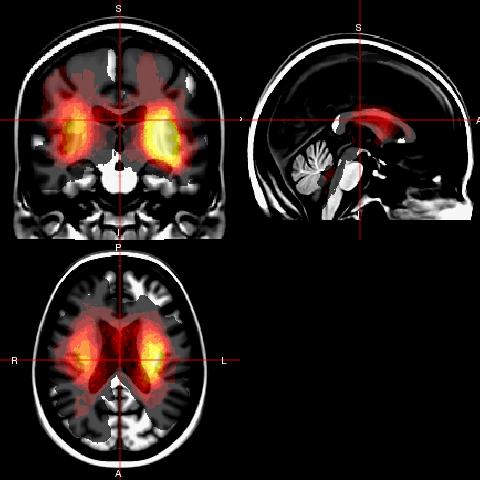
\includegraphics[width=.48\textwidth]{reoriented_Binary_Sum_Image_t1_heat_overlay.png}
}

\caption{{\bf ICH engagement prevalence.} A non-spatial histogram of proportion of patients (\protect\subref{prop:hist}) show the majority of voxels have a low prevalence (median: 3\%), while some voxels ($V = 5685$) have a high prevalence over 40\%. Voxels with no prevalence are excluded.  In (\protect\subref{prop:img}), these proportions are represented in a 3D histogram (right side of image is left side of brain) overlaid on an MRI T1 template.  More hemorrhages are in the left side of the brain.  ICH is also more localized in the middle of the brain, with few extensions in the anterior and posterior areas.   The interactive version of this figure is located at \url{http://muschellij2.github.io/CT_Pipeline/index.html}.}
  \label{fig:StrokeHist}
\end{figure}




\begin{figure}[H]
\centering
 \subfloat{
 \label{mods:m1}
 }
  \hfill
  \subfloat{
 \label{mods:m2}
 }
\newline
  \hfill
  \subfloat{
 \label{mods:m5}
 }
  \hfill
  \subfloat{
 \label{mods:m6}
 } 
  \caption{{\bf P-value maps for the voxel-wise NIHSS models.}  In the unadjusted (panel~\protect\subref{mods:m1}) or sex-adjusted (not shown) linear models, voxels with the smallest p-values appear medial near the lateral ventricles.  In age-adjusted (panel~\protect\subref{mods:m2}), total baseline ICH volume-adjusted (not shown), or age and volume-adjusted (panel~\protect\subref{mods:m5}), the p-values relating to NIHSS scores appear higher (more bluish).  The Wilcoxon rank-sum test (\protect\subref{mods:m6}) have smaller p-values for the same area compared to the unadjusted linear model. }
  \label{f:mods}
\end{figure}




\begin{figure}[H]
\centering
  \hfill
  \subfloat{
 \label{pvals:nihss}
 }
  \hfill
  \subfloat{
 \label{pvals:gcs}
 } 
 \newline
  \hfill
  \subfloat{
 \label{pvals:regnihss}
 }
  \hfill
  \subfloat{
 \label{pvals:reggcs}
 } 
 \newline 
  \caption{{\bf Highest Predictive Region (HPR) Analysis.}  Panels~\protect\subref{pvals:nihss} and~\protect\subref{pvals:gcs} correspond to the HPR for the top-performing model for NIHSS and GCS scores.  The HPR in (\protect\subref{pvals:nihss}) represents a p-value threshold of $.0100$ ($19047$ voxels) for the voxel-wise p-value of ICH on NIHSS. The HPR in (\protect\subref{pvals:gcs}) represents $1000$ with the lowest p-values for the voxel-wise ICH on GCS score regressions, corresponding to a p-value threshold of $.0002$.
    Panels~\protect\subref{pvals:regnihss} and~\protect\subref{pvals:reggcs} plot the relationship of the HPR coverage and severity score.  The red line represents a linear fit and the blue line represents a LOESS fit.  The larger the HPR coverage the higher (more severe stroke) NIHSS score and the lower (deeper unconsciousness) the GCS score.  
}
  \label{f:roi}
\end{figure}





\newpage

\section{Tables}






% latex table generated in R 3.1.0 by xtable 1.7-3 package
% Tue Jul  8 13:54:14 2014
\begin{table}[ht]
\centering
\begin{tabular}{lc}
  \hline {\bf Variable (N = 111)} & {\bf N (\%) or Mean (SD)} \\ 
  \hline
Age in Years: Mean (SD) & 60.8 (11.2) \\ 
   \hline
Gender: Female & 35 (31.5\%) \\ 
   \hline
NIHSS Score: Mean (SD) & 22.1 (8.7) \\ 
   \hline
GCS Score: Mean (SD) & 10.0 (3.0) \\ 
   \hline
Race &  \\ 
   \hline
\text{  } Caucasian not Hispanic & 59 (53.2\%) \\ 
   \hline
\text{  } African American not Hispanic & 35 (31.5\%) \\ 
   \hline
\text{  } Hispanic & 12 (10.8\%) \\ 
   \hline
\text{  } Asian or Pacific Islander & 5 (4.5\%) \\ 
   \hline
Reader-Classified ICH Location &  \\ 
   \hline
\text{  } Putamen & 68 (61.3\%) \\ 
   \hline
\text{  } Lobar & 33 (29.7\%) \\ 
   \hline
\text{  } Globus Pallidus & 6 (5.4\%) \\ 
   \hline
\text{  } Thalamus & 4 (3.6\%) \\ 
   \hline
\end{tabular}
\caption{Descriptive statistics of the demographic information on the patients.} 
\label{t:dem}
\end{table}






% % latex table generated in R 3.1.0 by xtable 1.7-3 package
% Tue Jul 15 14:35:47 2014
\begin{table}[H]
\centering
\begin{tabular}{rr|cccc}
  \hline
{\bf Number of Voxels} & {\bf P-value} & {\bf Adjusted R$^2$} & {\bf R$^2$} & {\bf AIC} & {\bf RMSE} \\ 
  \hline
Location Model &  & 0.129 & 0.178 & 18.60 & 8.116 \\ 
  1000 & .0005 & 0.236 & 0.265 & 2.47 & 7.598 \\ 
  2000 & .0009 & 0.234 & 0.263 & 2.81 & 7.610 \\ 
  2422 & .0010 & 0.247 & 0.275 & 0.98 & 7.545 \\ 
  3000 & .0013 & 0.244 & 0.272 & 1.46 & 7.562 \\ 
  19047 & .0100 & 0.254 & 0.282 & 0.00 & 7.511 \\ 
  47736 & .0500 & 0.248 & 0.276 & 0.77 & 7.538 \\ 
   \hline
\end{tabular}
\caption{Table of model-fit measures for NIHSS score: reader-based location model vs. CT voxel-based HPR coverage models. We see that the model using a p-value threshold of .0100 corresponds to the best model on all model-fit measures: adjusted and unadjusted $R^2$ are the highest; AIC, and RMSE are the smallest.  The models using HPR coverage have comparable fit measures, but each HPR coverage model outperforms the reader-based location model, notably in the $R^2$ measures.  Thus, we infer that using CT-based regions of interest may help in prediction of NIHSS score.} 
\label{t:nihss}
\end{table}










% % latex table generated in R 3.1.0 by xtable 1.7-3 package
% Tue Jul  8 13:54:14 2014
\begin{table}[H]
\centering
\begin{tabular}{rr|cccc}
  \hline
{\bf Number of Voxels} & {\bf P-value} & {\bf Adjusted R$^2$} & {\bf R$^2$} & {\bf AIC} & {\bf RMSE} \\ 
  \hline
Location Model &  & 0.069 & 0.120 & 20.51 & 2.914 \\ 
  1000 & .0002 & 0.214 & 0.243 & 0.00 & 2.677 \\ 
  2000 & .0004 & 0.213 & 0.242 & 0.09 & 2.678 \\ 
  3000 & .0006 & 0.212 & 0.241 & 0.25 & 2.680 \\ 
  4669 & .0010 & 0.212 & 0.241 & 0.23 & 2.680 \\ 
  22858 & .0100 & 0.191 & 0.221 & 3.17 & 2.716 \\ 
  52368 & .0500 & 0.166 & 0.197 & 6.44 & 2.757 \\ 
   \hline
\end{tabular}
\caption{Table of model-fit measures for GCS score: reader-based location model vs. CT voxel-based HPR coverage models. We see that the model using a using the voxels with lowest 1000 p-values corresponds to the best model on all model-fit measures: adjusted and unadjusted $R^2$ are the highest; AIC, and RMSE are the smallest.  The models using HPR coverage have comparable fit measures, but each HPR coverage model outperforms the reader-based location model, notably in the $R^2$ measures.  Thus, we infer that using CT-based regions of interest may help in prediction of NIHSS score.} 
\label{t:gcs}
\end{table}


% latex table generated in R 3.1.0 by xtable 1.7-3 package
% Tue Jul 15 14:35:48 2014
\begin{table}[H]
\centering
\begin{tabular}{rr|cccc}
  \hline
{\bf Number of Voxels} & {\bf P-value} & {\bf Adjusted R$^2$} & {\bf R$^2$} & {\bf AIC} & {\bf RMSE} \\ 
  \hline \multicolumn{6}{c}{\bf NIHSS Score }\\ 
 \hline
\bf Location Model & \bf  & 0.129 & 0.178 & 18.60 & 8.116 \\ 
  \bf 1000 & \bf .0005 & 0.236 & 0.265 & 2.47 & 7.598 \\ 
  \bf 2000 & \bf .0009 & 0.234 & 0.263 & 2.81 & 7.610 \\ 
  \bf 2422 & \bf .0010 & 0.247 & 0.275 & 0.98 & 7.545 \\ 
  \bf 3000 & \bf .0013 & 0.244 & 0.272 & 1.46 & 7.562 \\ 
  \bf 19047 & \bf .0100 & 0.254 & 0.282 & 0.00 & 7.511 \\ 
  \bf 47736 & \bf .0500 & 0.248 & 0.276 & 0.77 & 7.538 \\ 
    \hline\hline \multicolumn{6}{c}{\bf GCS Score }\\ 
\hline \bf Location Model & \bf  & 0.069 & 0.120 & 20.51 & 2.914 \\ 
  \bf 1000 & \bf .0002 & 0.214 & 0.243 & 0.00 & 2.677 \\ 
  \bf 2000 & \bf .0004 & 0.213 & 0.242 & 0.09 & 2.678 \\ 
  \bf 3000 & \bf .0006 & 0.212 & 0.241 & 0.25 & 2.680 \\ 
  \bf 4669 & \bf .0010 & 0.212 & 0.241 & 0.23 & 2.680 \\ 
  \bf 22858 & \bf .0100 & 0.191 & 0.221 & 3.17 & 2.716 \\ 
  \bf 52368 & \bf .0500 & 0.166 & 0.197 & 6.44 & 2.757 \\ 
   \hline
\end{tabular}
\caption{Table of model-fit measures for GCS and NIHSS score: reader-based location model vs. CT voxel-based HPR coverage models. We see that the model using a using the voxels using an HPR with a p-value threshold of .0100 for NIHSS and the HPR with the lowest 1000 p-values GCS corresponds to the best models on all model-fit measures: adjusted and unadjusted $R^2$ are the highest; AIC, and RMSE are the smallest.  The models using HPR coverage have comparable fit measures, but each HPR coverage model outperforms the reader-based location model, notably in the $R^2$ measures.  Thus, we infer that using CT-based regions of interest may help in prediction of NIHSS and GCS scores.} 
\label{t:allres}
\end{table}









%% latex table generated in R 3.1.0 by xtable 1.7-3 package
% Wed Jul 23 12:03:51 2014
\begin{table}[ht]
\centering
\begin{tabular}{lccc}
  \hline
Area & Population Prevalence & NIHSS HPR & GCS HPR \\ 
  \hline
CSF & 7.9 & 10.0 & 4.2 \\ 
  Insular & 4.7 &  &  \\ 
  Superior temporal gyrus & 3.8 &  &  \\ 
  Putamen left & 3.0 &  &  \\ 
  Insular right & 2.9 &  &  \\ 
  External capsule left & 2.3 &  &  \\ 
  Superior corona radiata left & 1.9 & 11.8 & 27.9 \\ 
  Superior temporal wm left & 1.9 &  &  \\ 
  Superior corona radiata right & 1.8 &  &  \\ 
  Putamen right & 1.8 &  &  \\ 
  Posterior limb of internal capsule left &  & 10.1 & 3.9 \\ 
  Thalamus left &  & 7.6 & 33.9 \\ 
  Caudate nucleus left &  & 5.4 & 9.6 \\ 
  Superior longitudinal fasciculus left &  & 4.9 & 5.9 \\ 
  Globus pallidus left &  & 3.7 &  \\ 
  Anterior limb of internal capsule left &  & 3.6 &  \\ 
  Outside brain mask &  & 3.5 &  \\ 
  Anterior limb of internal capsule right &  & 3.0 &  \\ 
  Postcentral wm left &  &  & 6.7 \\ 
  Posterior corona radiata left &  &  & 3.1 \\ 
  Precentral wm left &  &  & 1.3 \\ 
  Supramarginal wm left &  &  & 1.1 \\ 
   \hline
\end{tabular}
\caption{Distribution of the top 10 areas of engagement} 
\label{t:breakdown}
\end{table}

% latex table generated in R 3.1.0 by xtable 1.7-3 package
% Wed Jul 23 12:03:51 2014
\begin{table}[ht]
\centering
\begin{tabular}{lccc}
  \hline
Area & Population Prevalence & NIHSS HPR & GCS HPR \\ 
  \hline
CSF & 7.9 & 10.9 & 4.2 \\ 
  Insular & 7.6 &  &  \\ 
  Superior temporal gyrus & 5.5 &  &  \\ 
  Putamen & 4.8 & 4.3 &  \\ 
  External capsule & 3.9 &  &  \\ 
  Superior corona radiata & 3.7 & 11.0 & 27.9 \\ 
  Precentral gyrus & 3.3 &  &  \\ 
  Precentral WM & 3.1 &  & 1.3 \\ 
  Superior temporal WM & 3.1 &  &  \\ 
  Posterior limb of internal capsule & 3.0 & 12.0 & 3.9 \\ 
  Thalamus &  & 10.1 & 33.9 \\ 
  Caudate nucleus &  & 8.4 & 9.6 \\ 
  Anterior limb of internal capsule &  & 6.8 &  \\ 
  Globus pallidus &  & 6.0 &  \\ 
  Superior longitudinal fasciculus &  & 4.5 & 5.9 \\ 
  Outside brain mask &  & 3.6 &  \\ 
  Postcentral WM &  &  & 6.7 \\ 
  Posterior corona radiata &  &  & 3.1 \\ 
  Supramarginal WM &  &  & 1.1 \\ 
   \hline
\end{tabular}
\caption{Distribution of the top 10 areas of engagement} 
\label{t:breakdown}
\end{table}





\clearpage
\newpage

\section{Figures}

\setcounter{figure}{0}

\begin{figure}[H]
\centering
  \subfloat{
  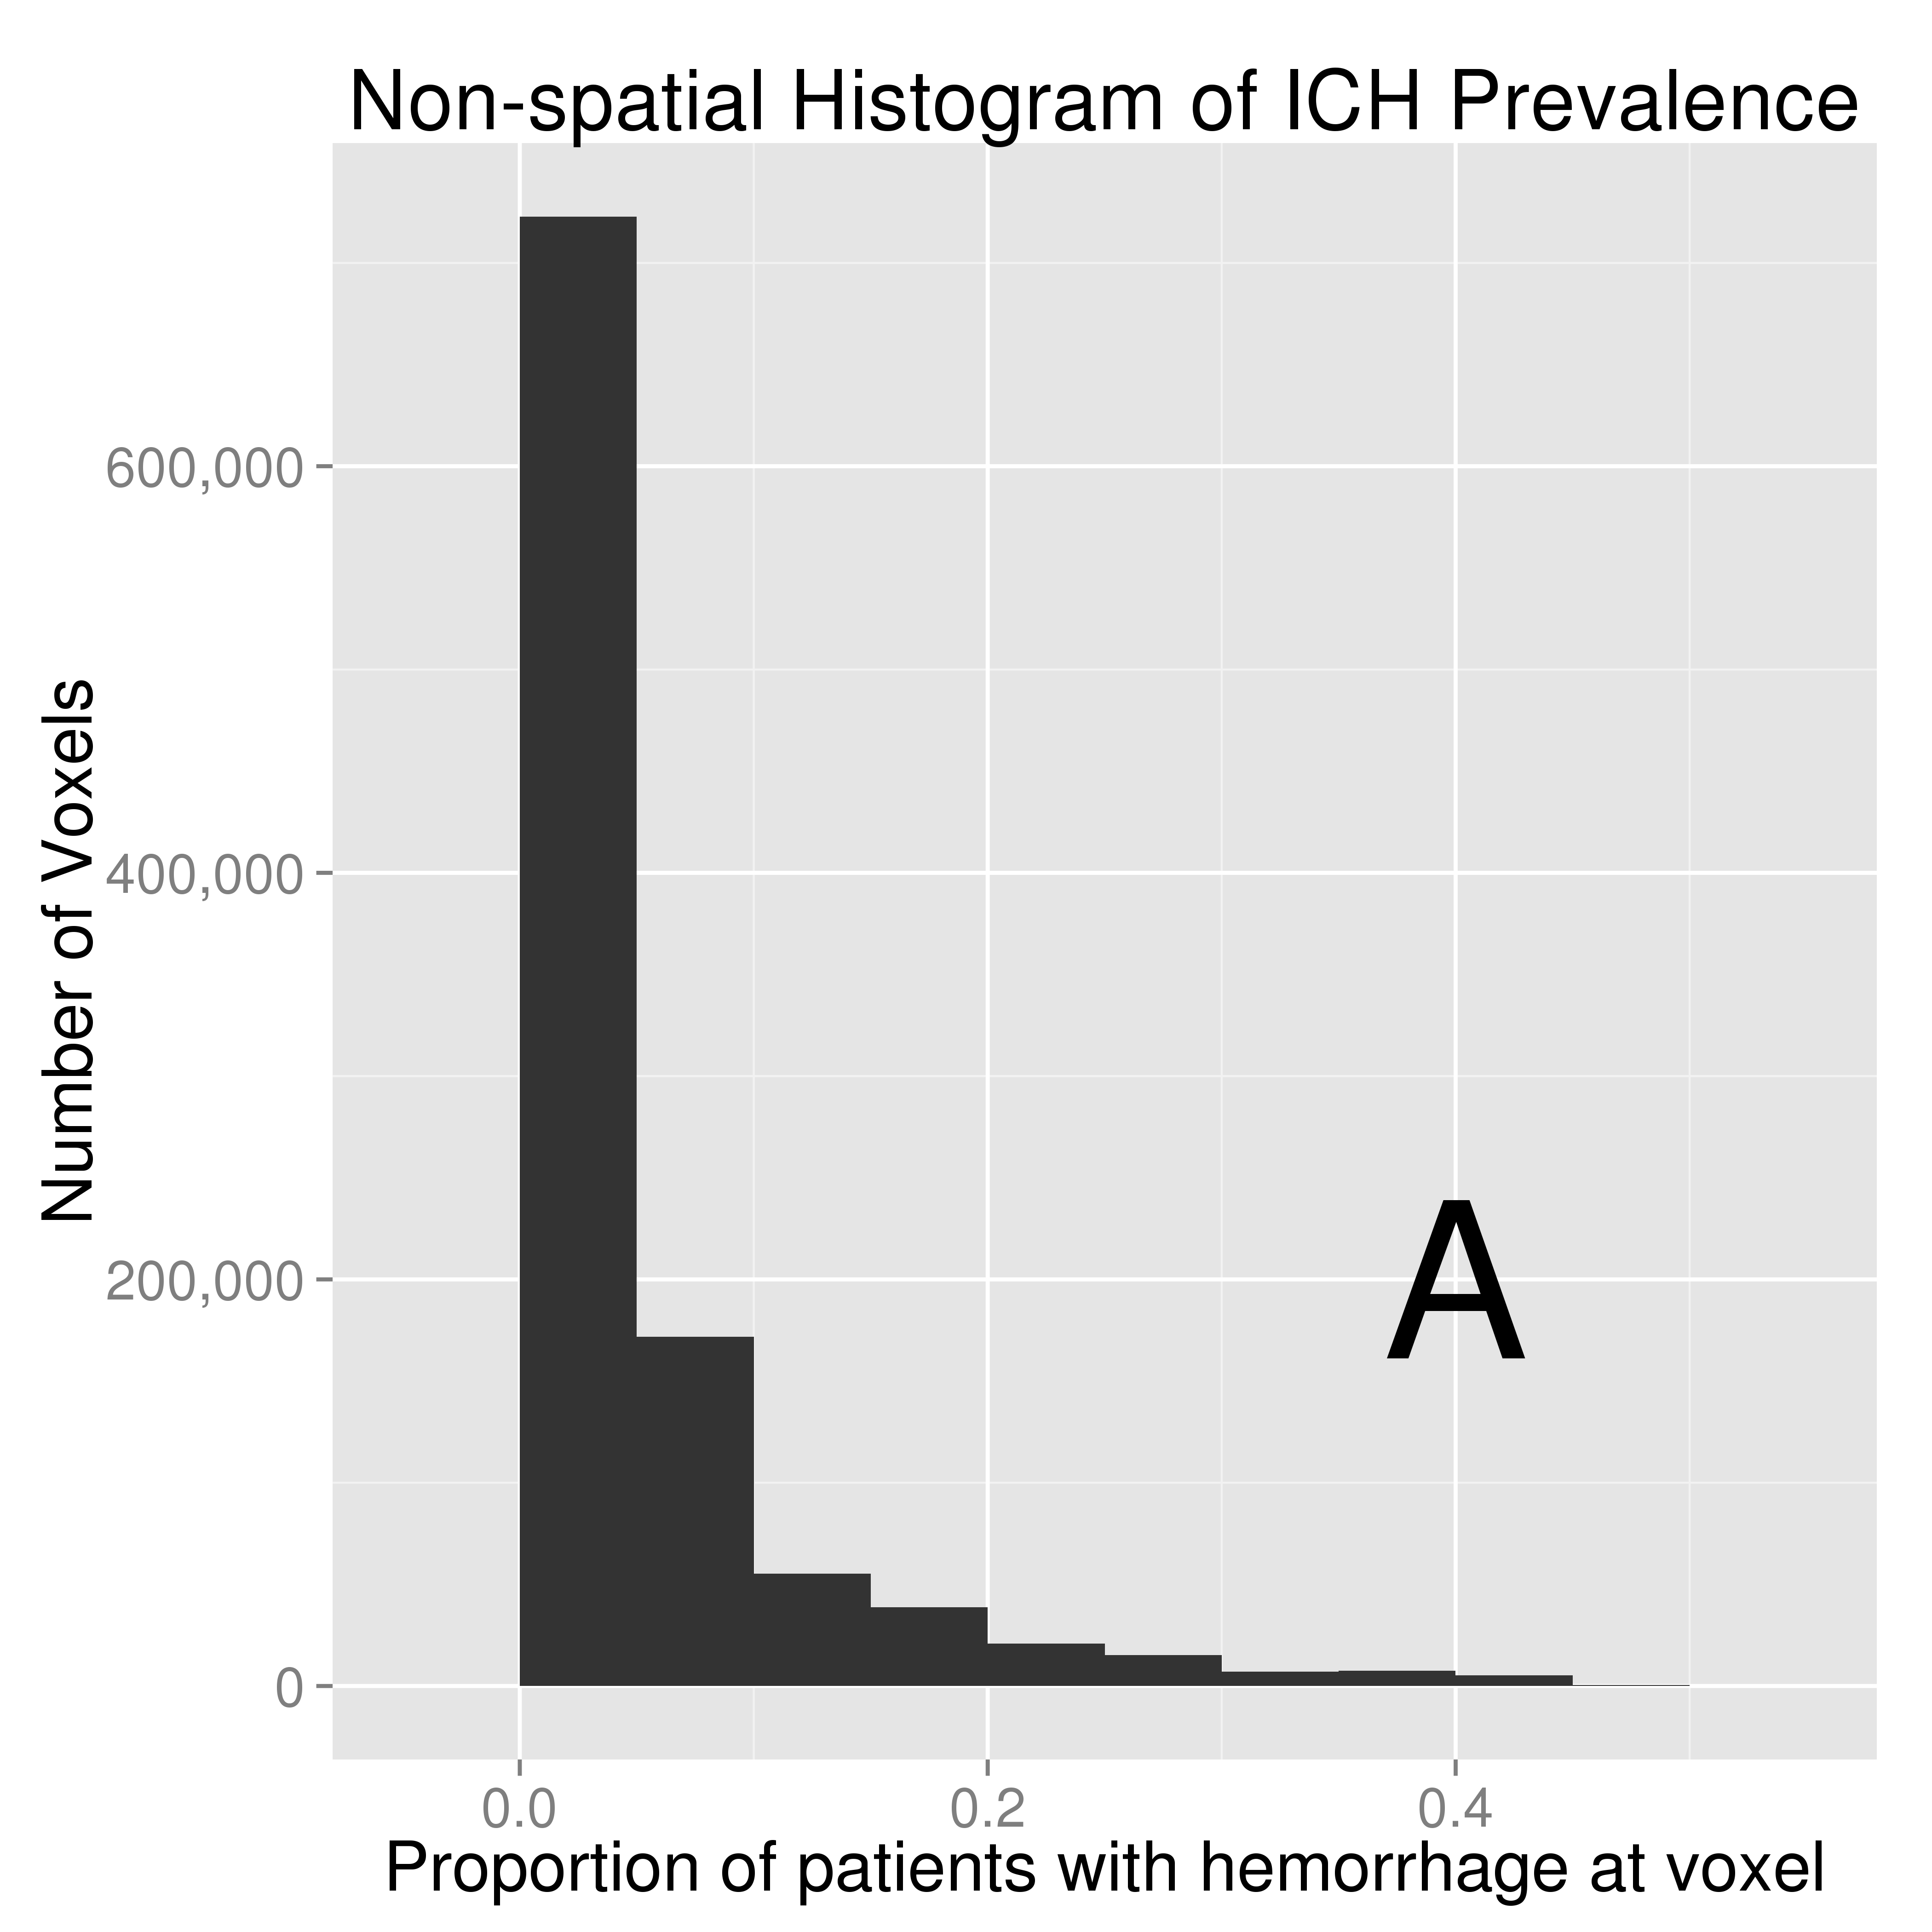
\includegraphics[width=.48\textwidth]{reoriented_Binary_Sum_Image_histogram.png}
}
  \subfloat{
%   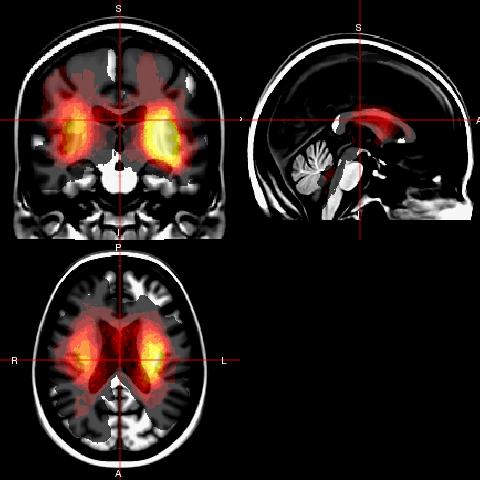
\includegraphics[width=.48\textwidth]{reoriented_Binary_Sum_Image_t1_heat_overlay.png}
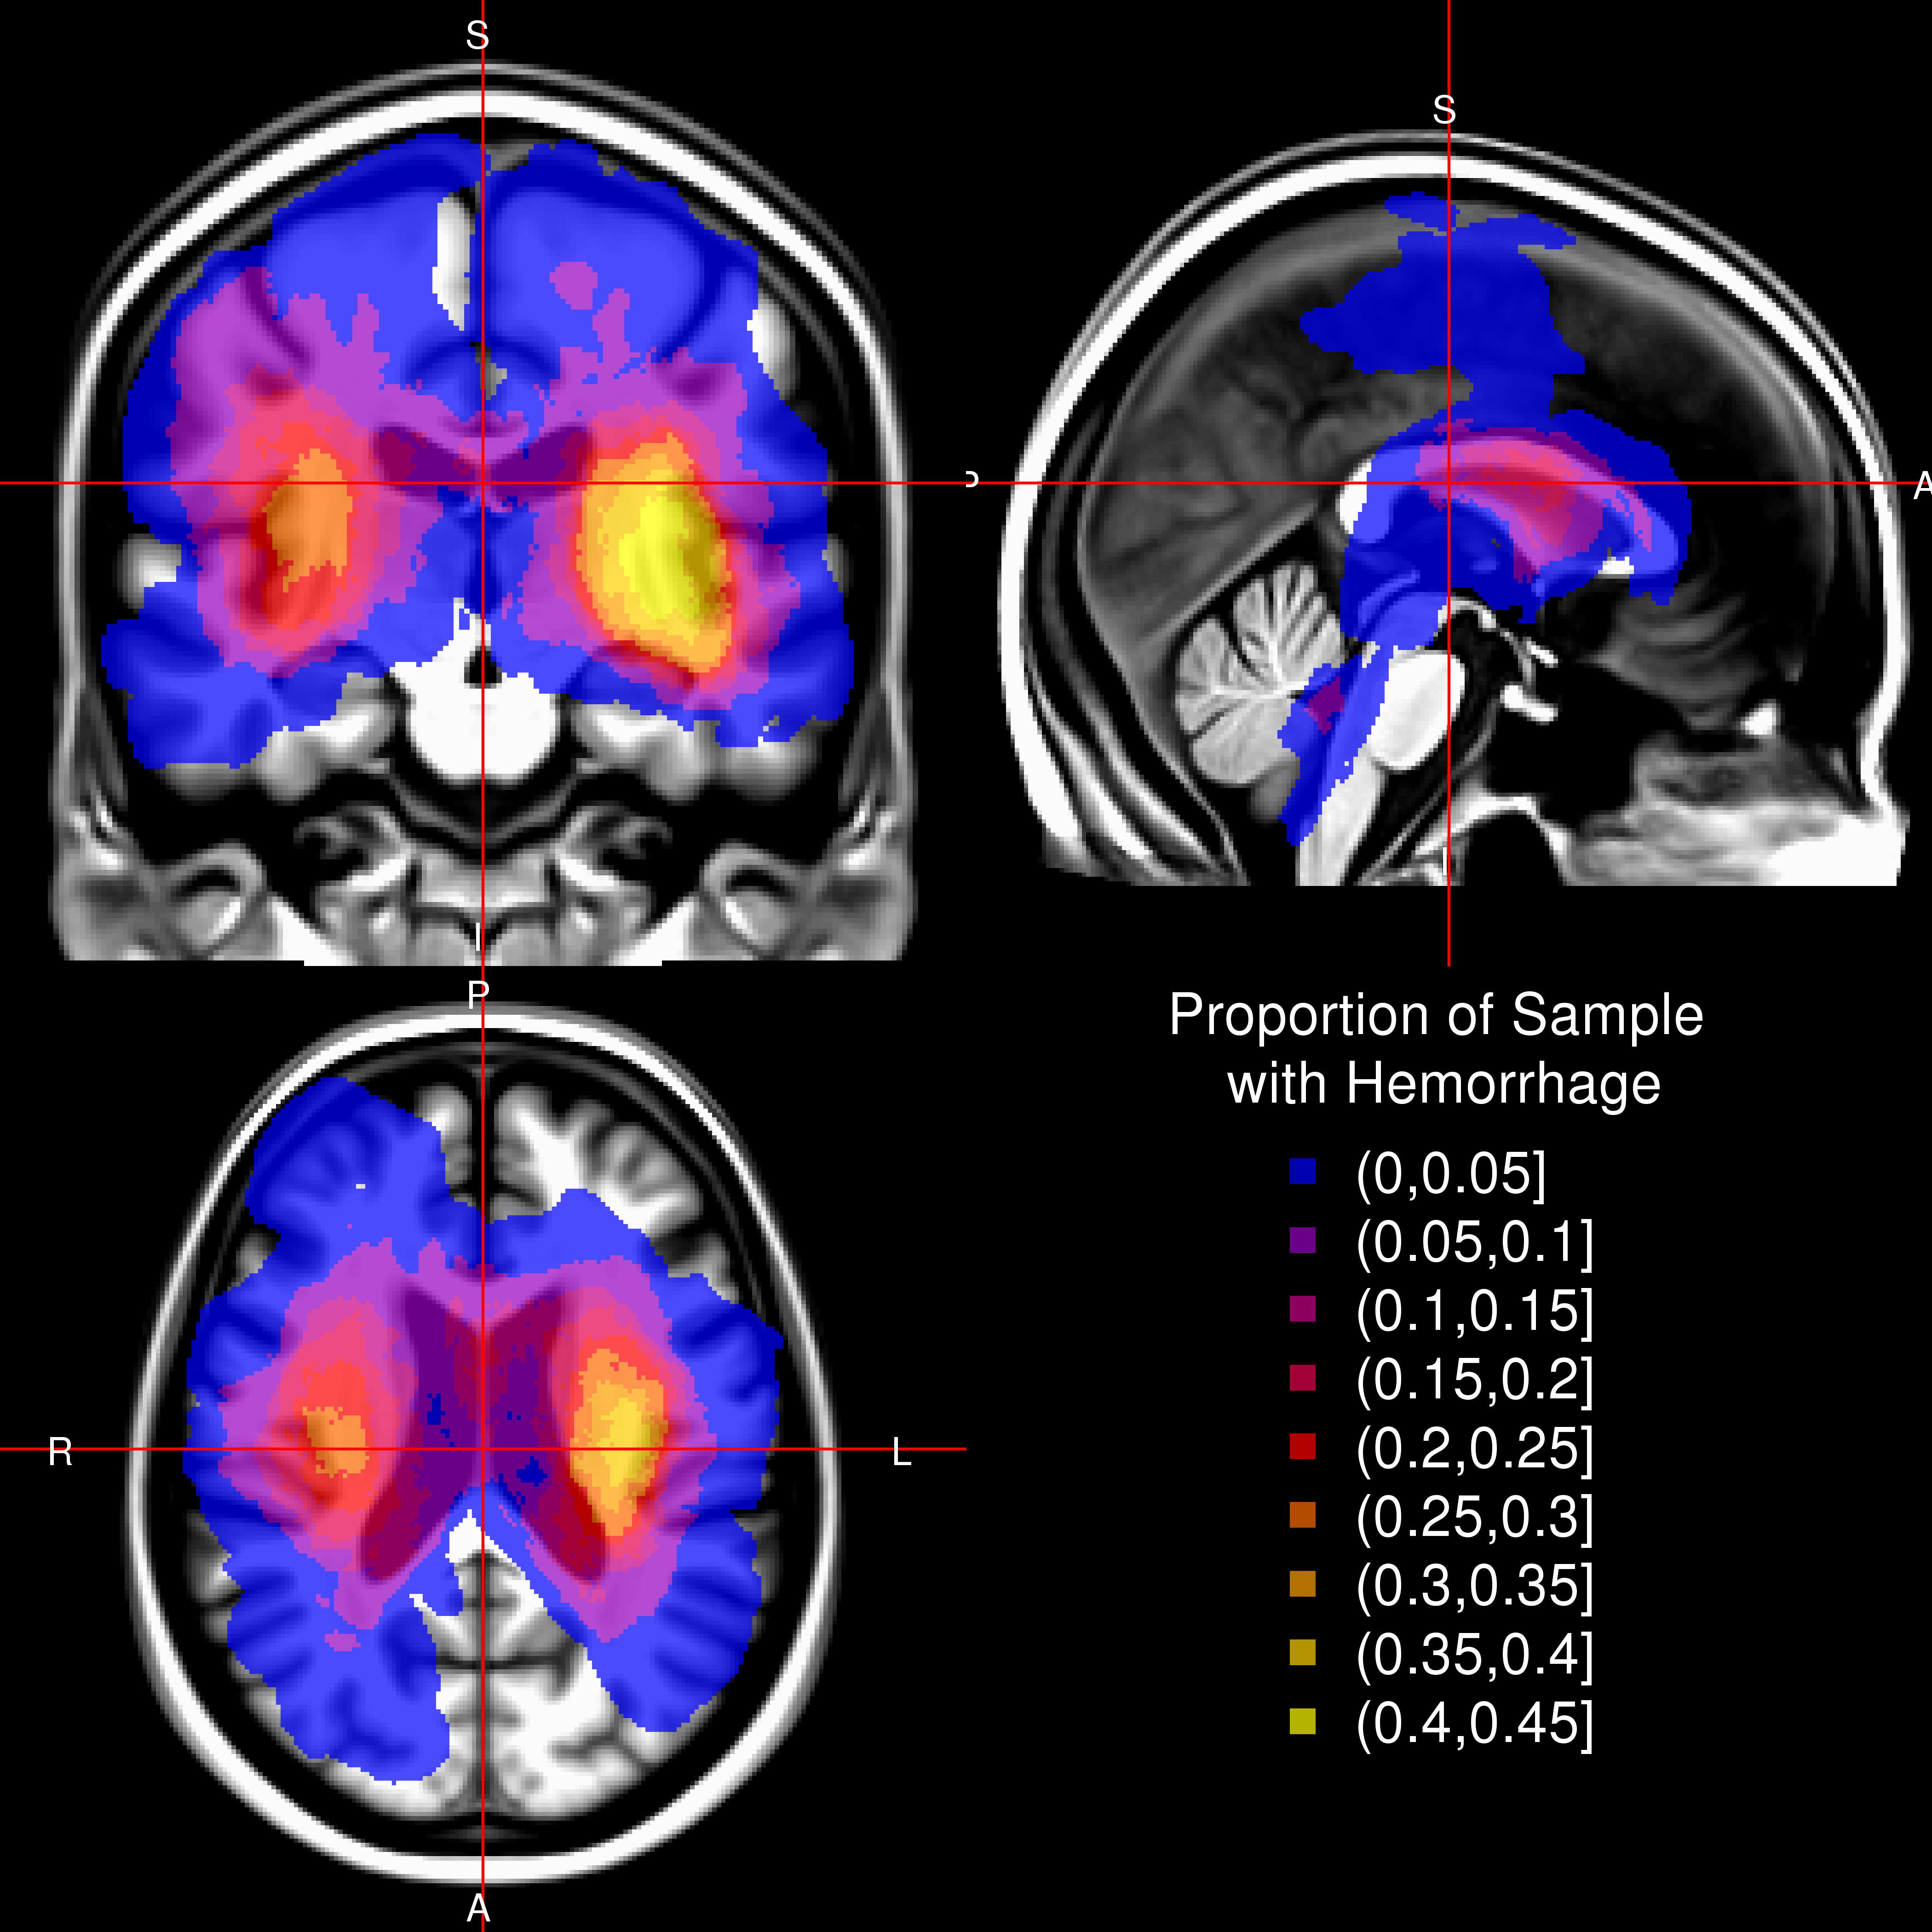
\includegraphics[width=.48\textwidth]{Figure4_Proportion.png}
}
\caption{}
\end{figure}




\begin{figure}[H]
\centering
 \subfloat{
 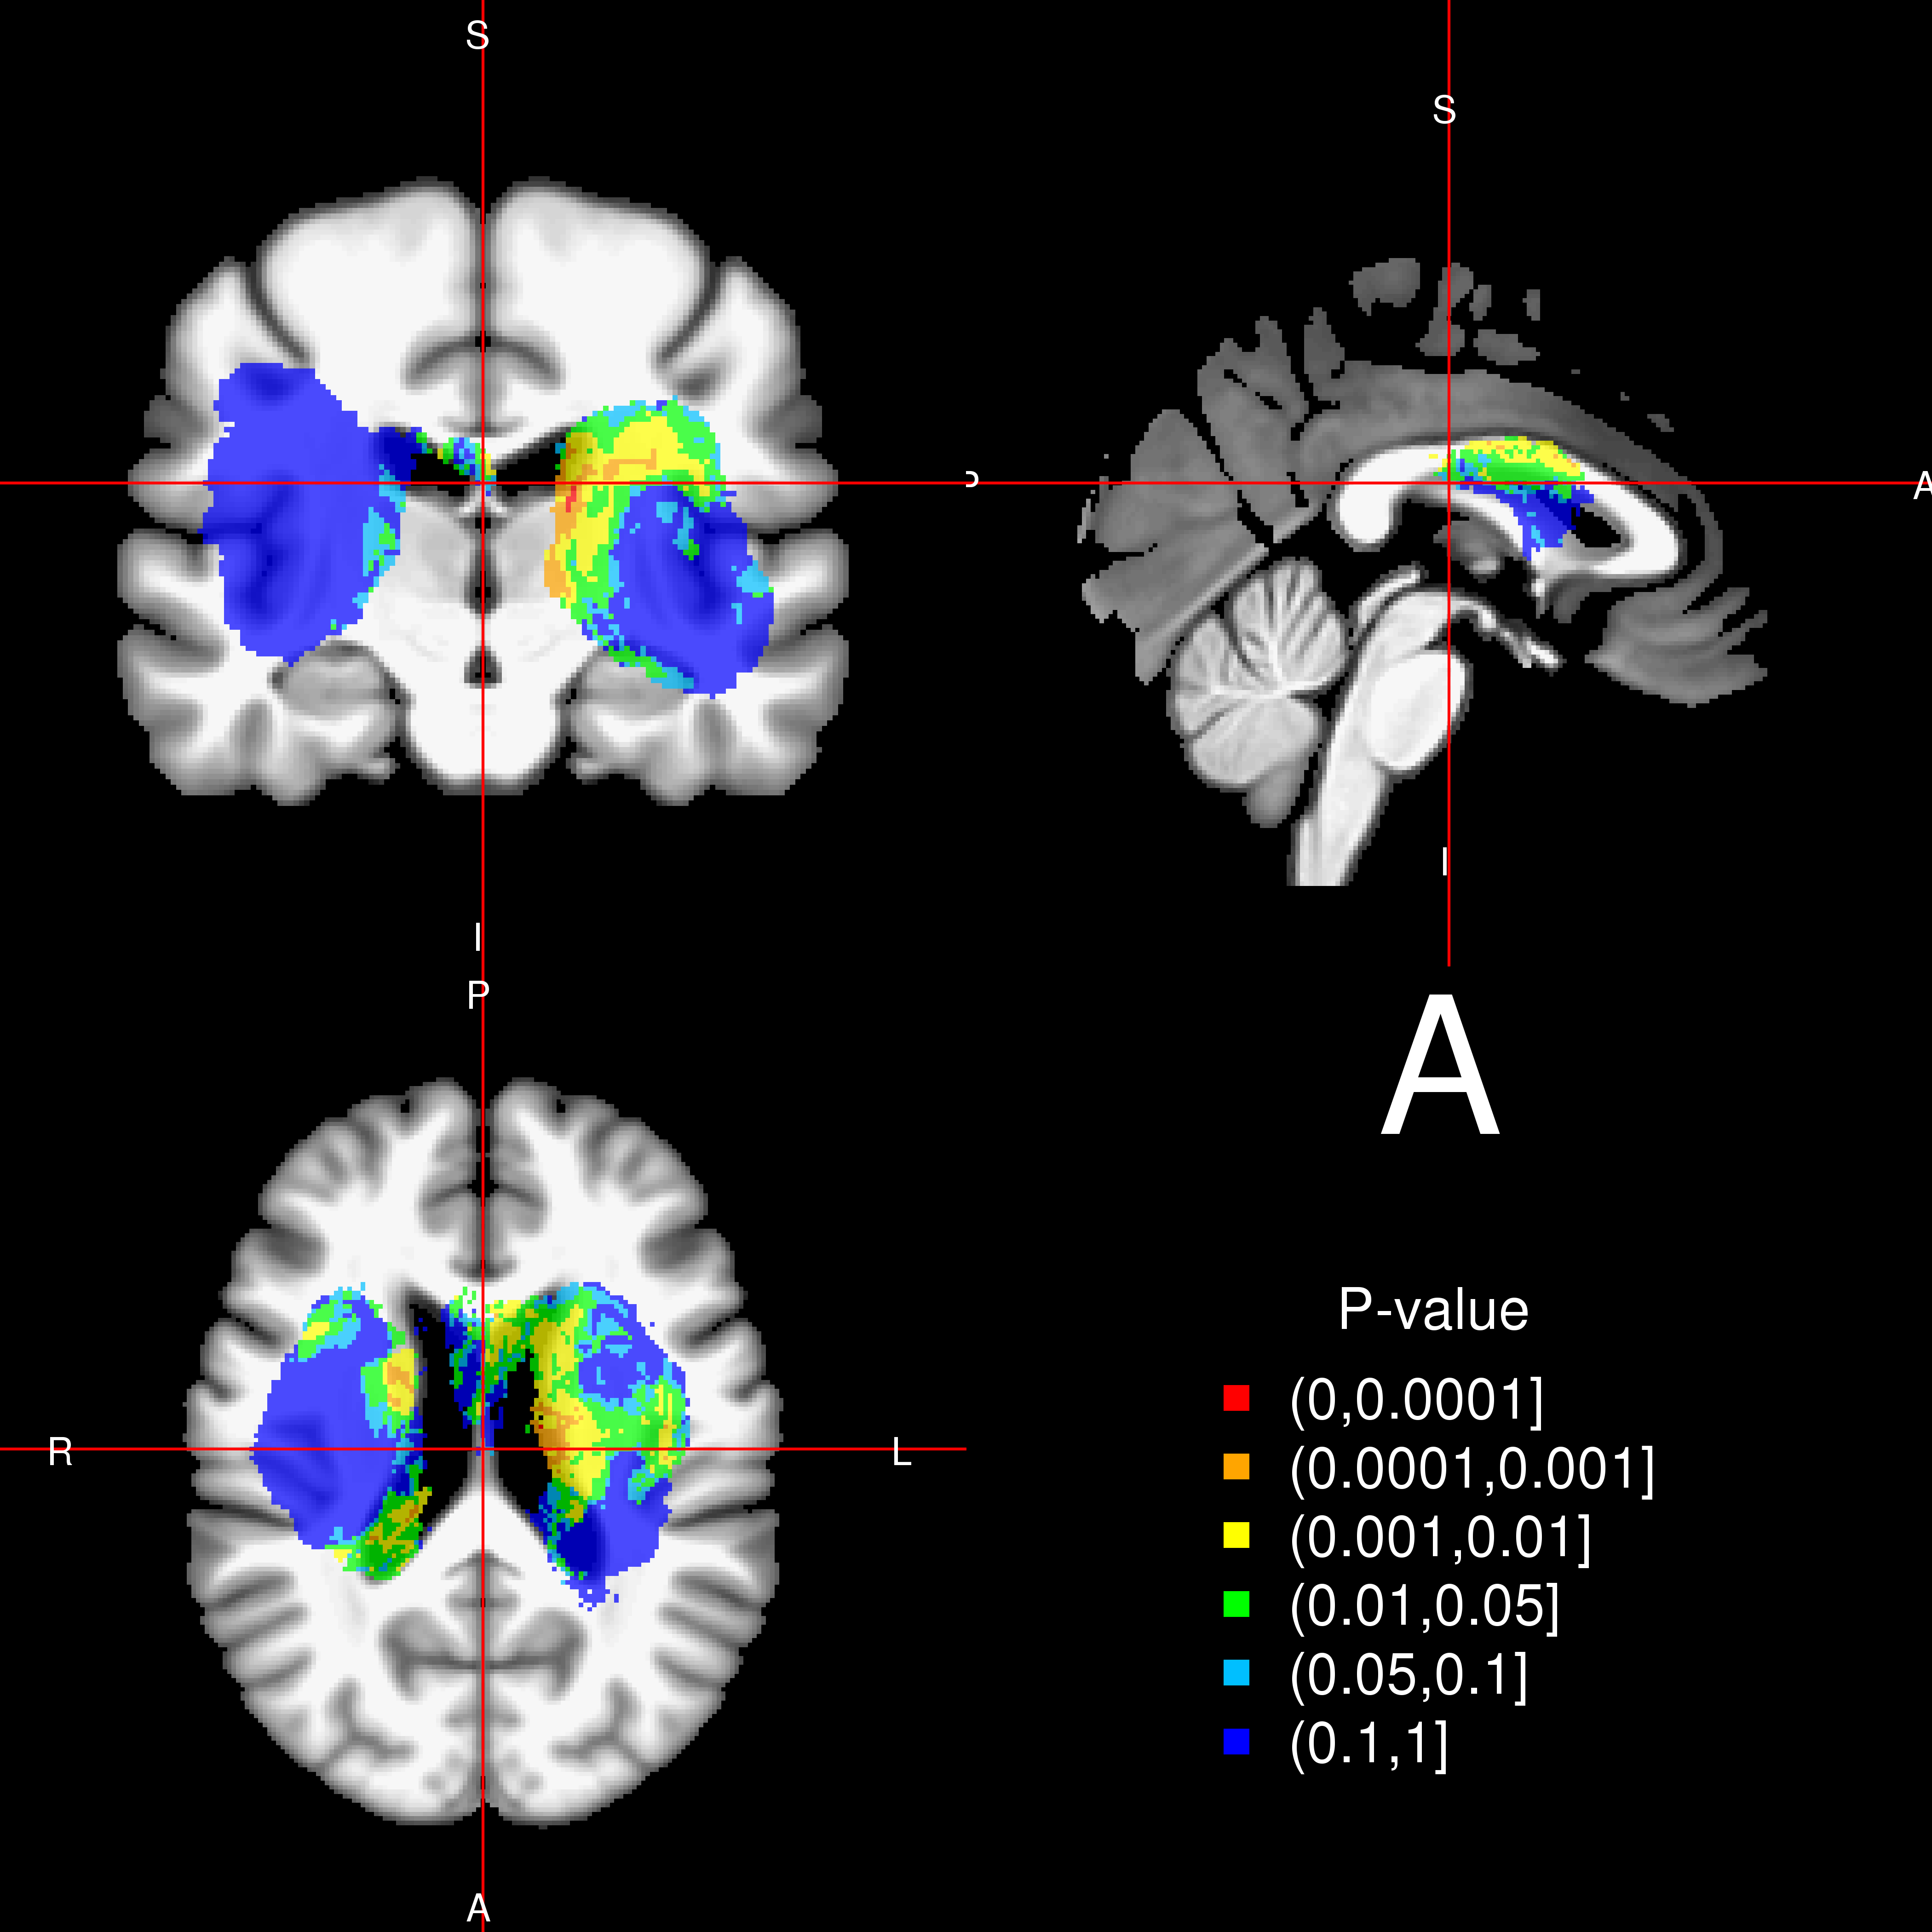
\includegraphics[width=.48\textwidth]{Regression_Map_heatcol1_t1_Final.png}
 }
  \hfill
  \subfloat{
 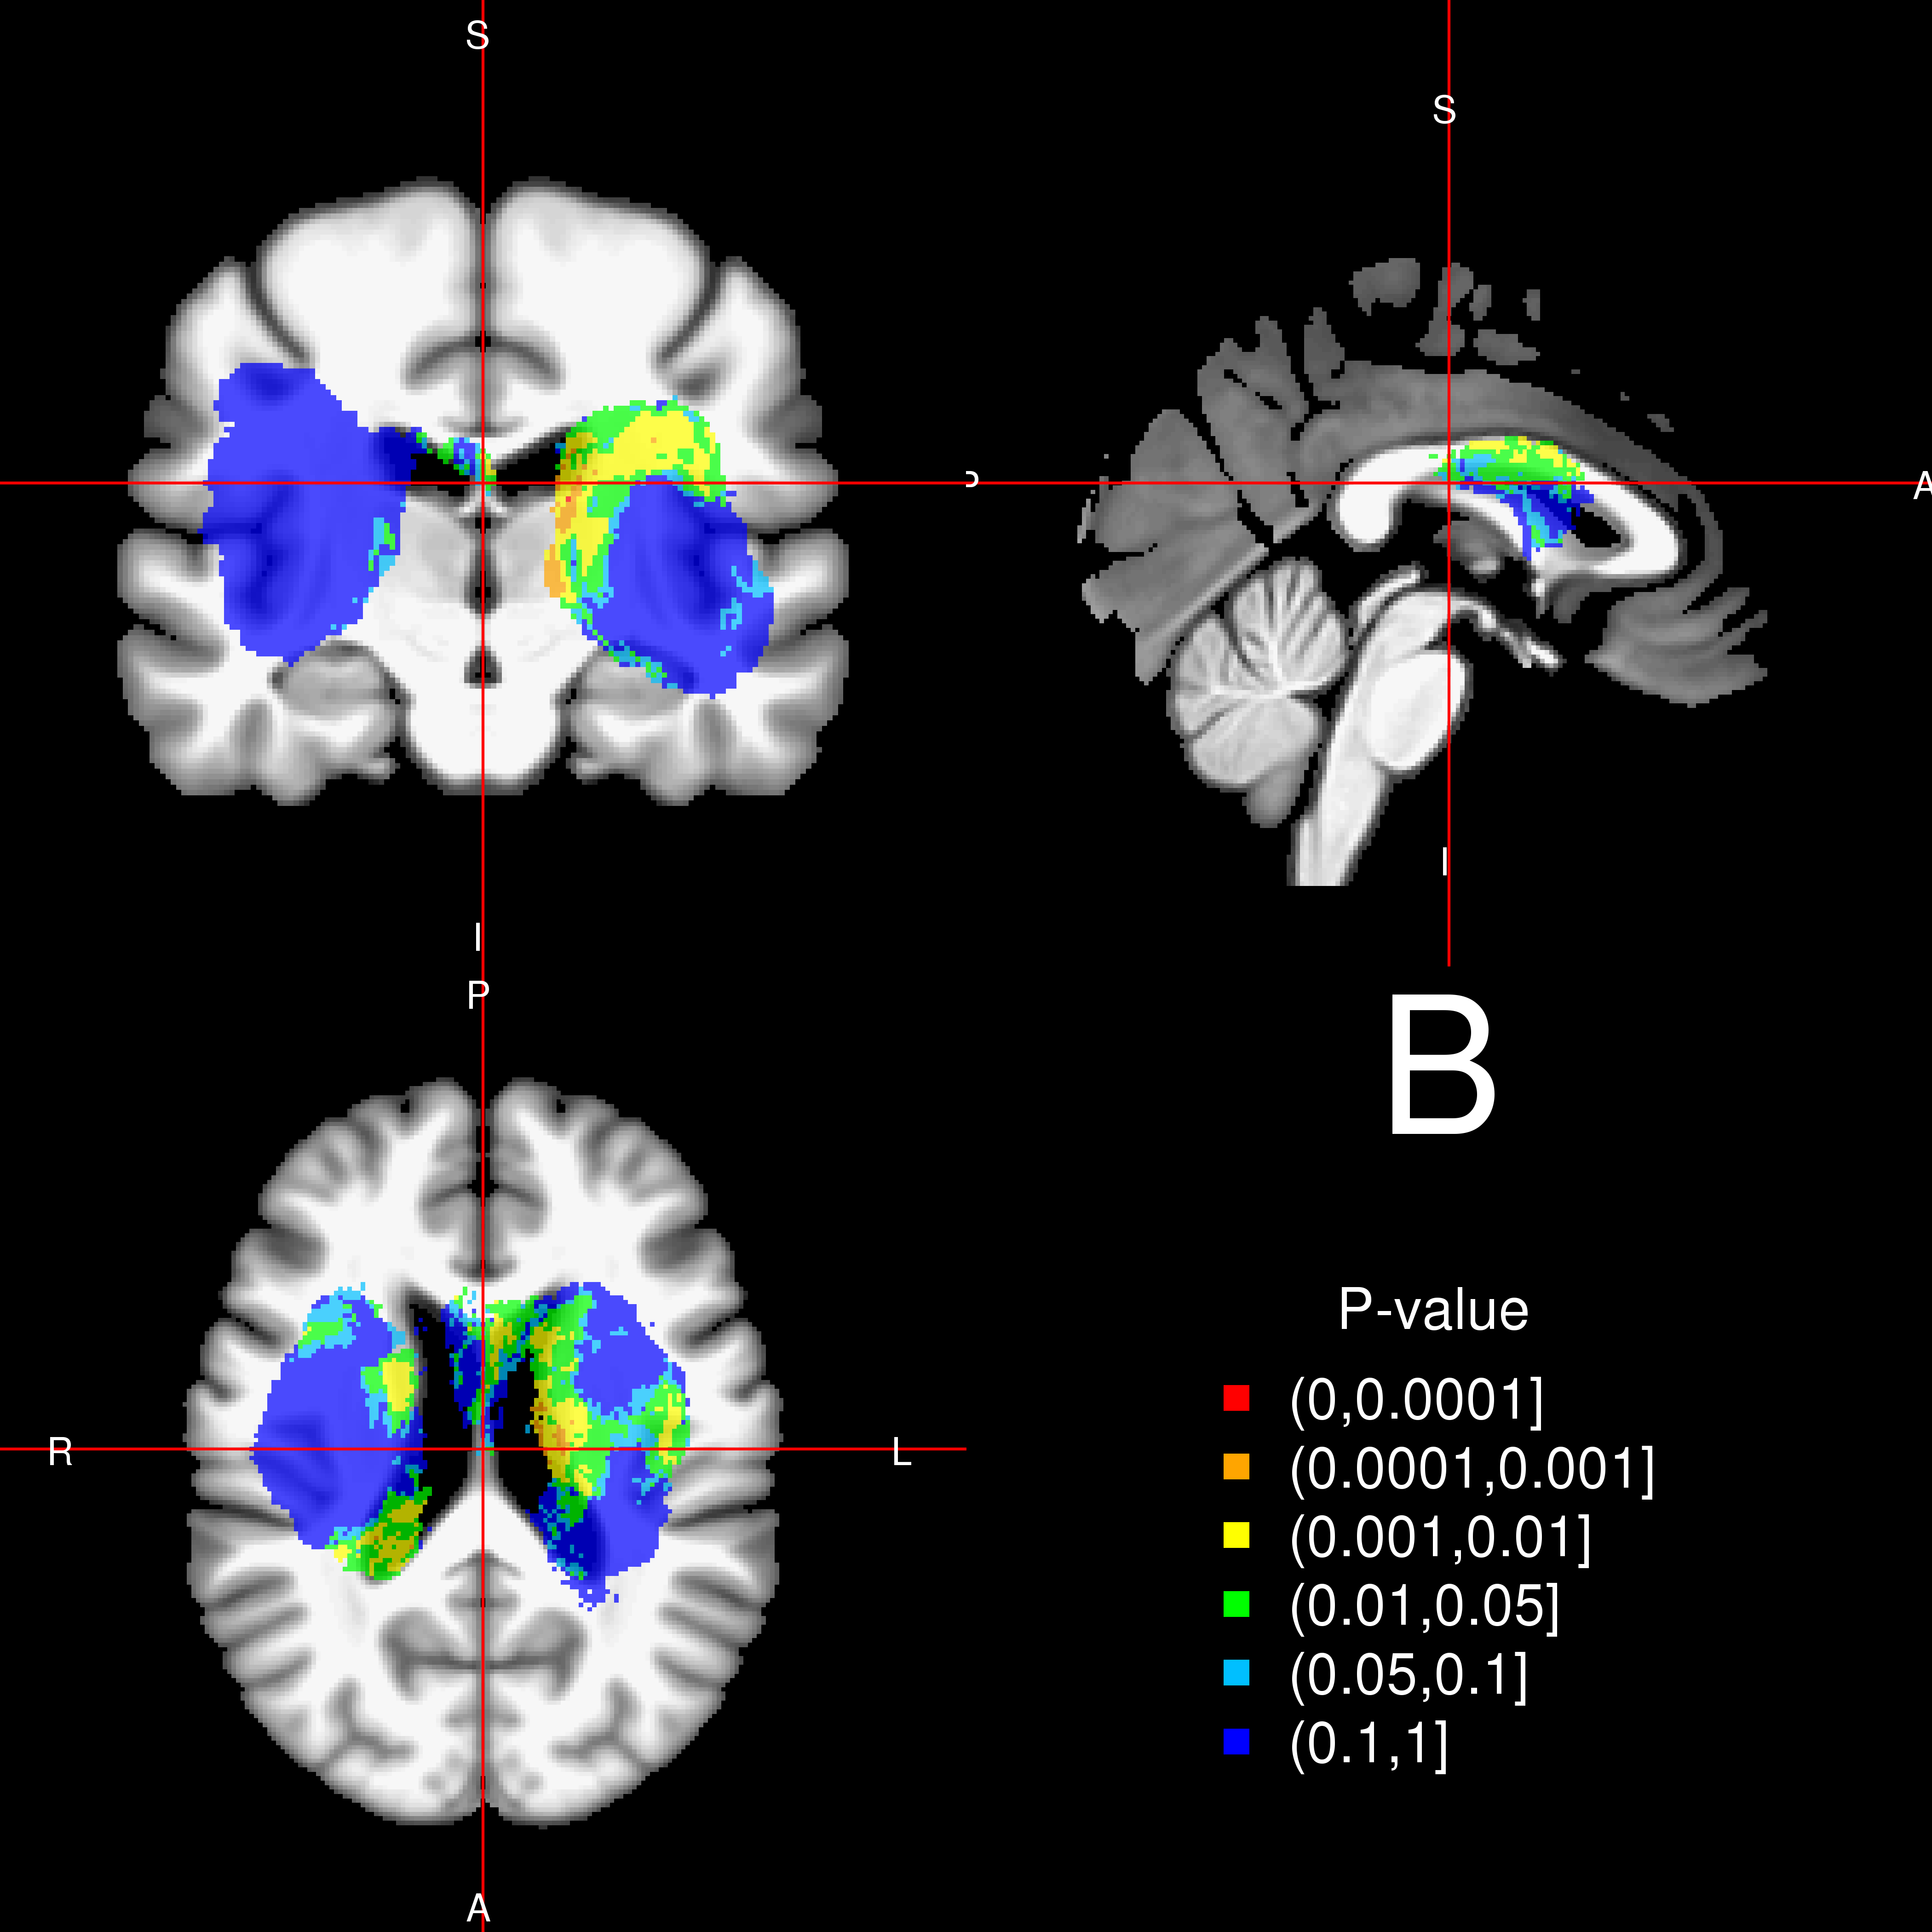
\includegraphics[width=.48\textwidth]{Regression_Map_heatcol2_t1_Final.png}
 }
\newline
  \hfill
  \subfloat{
 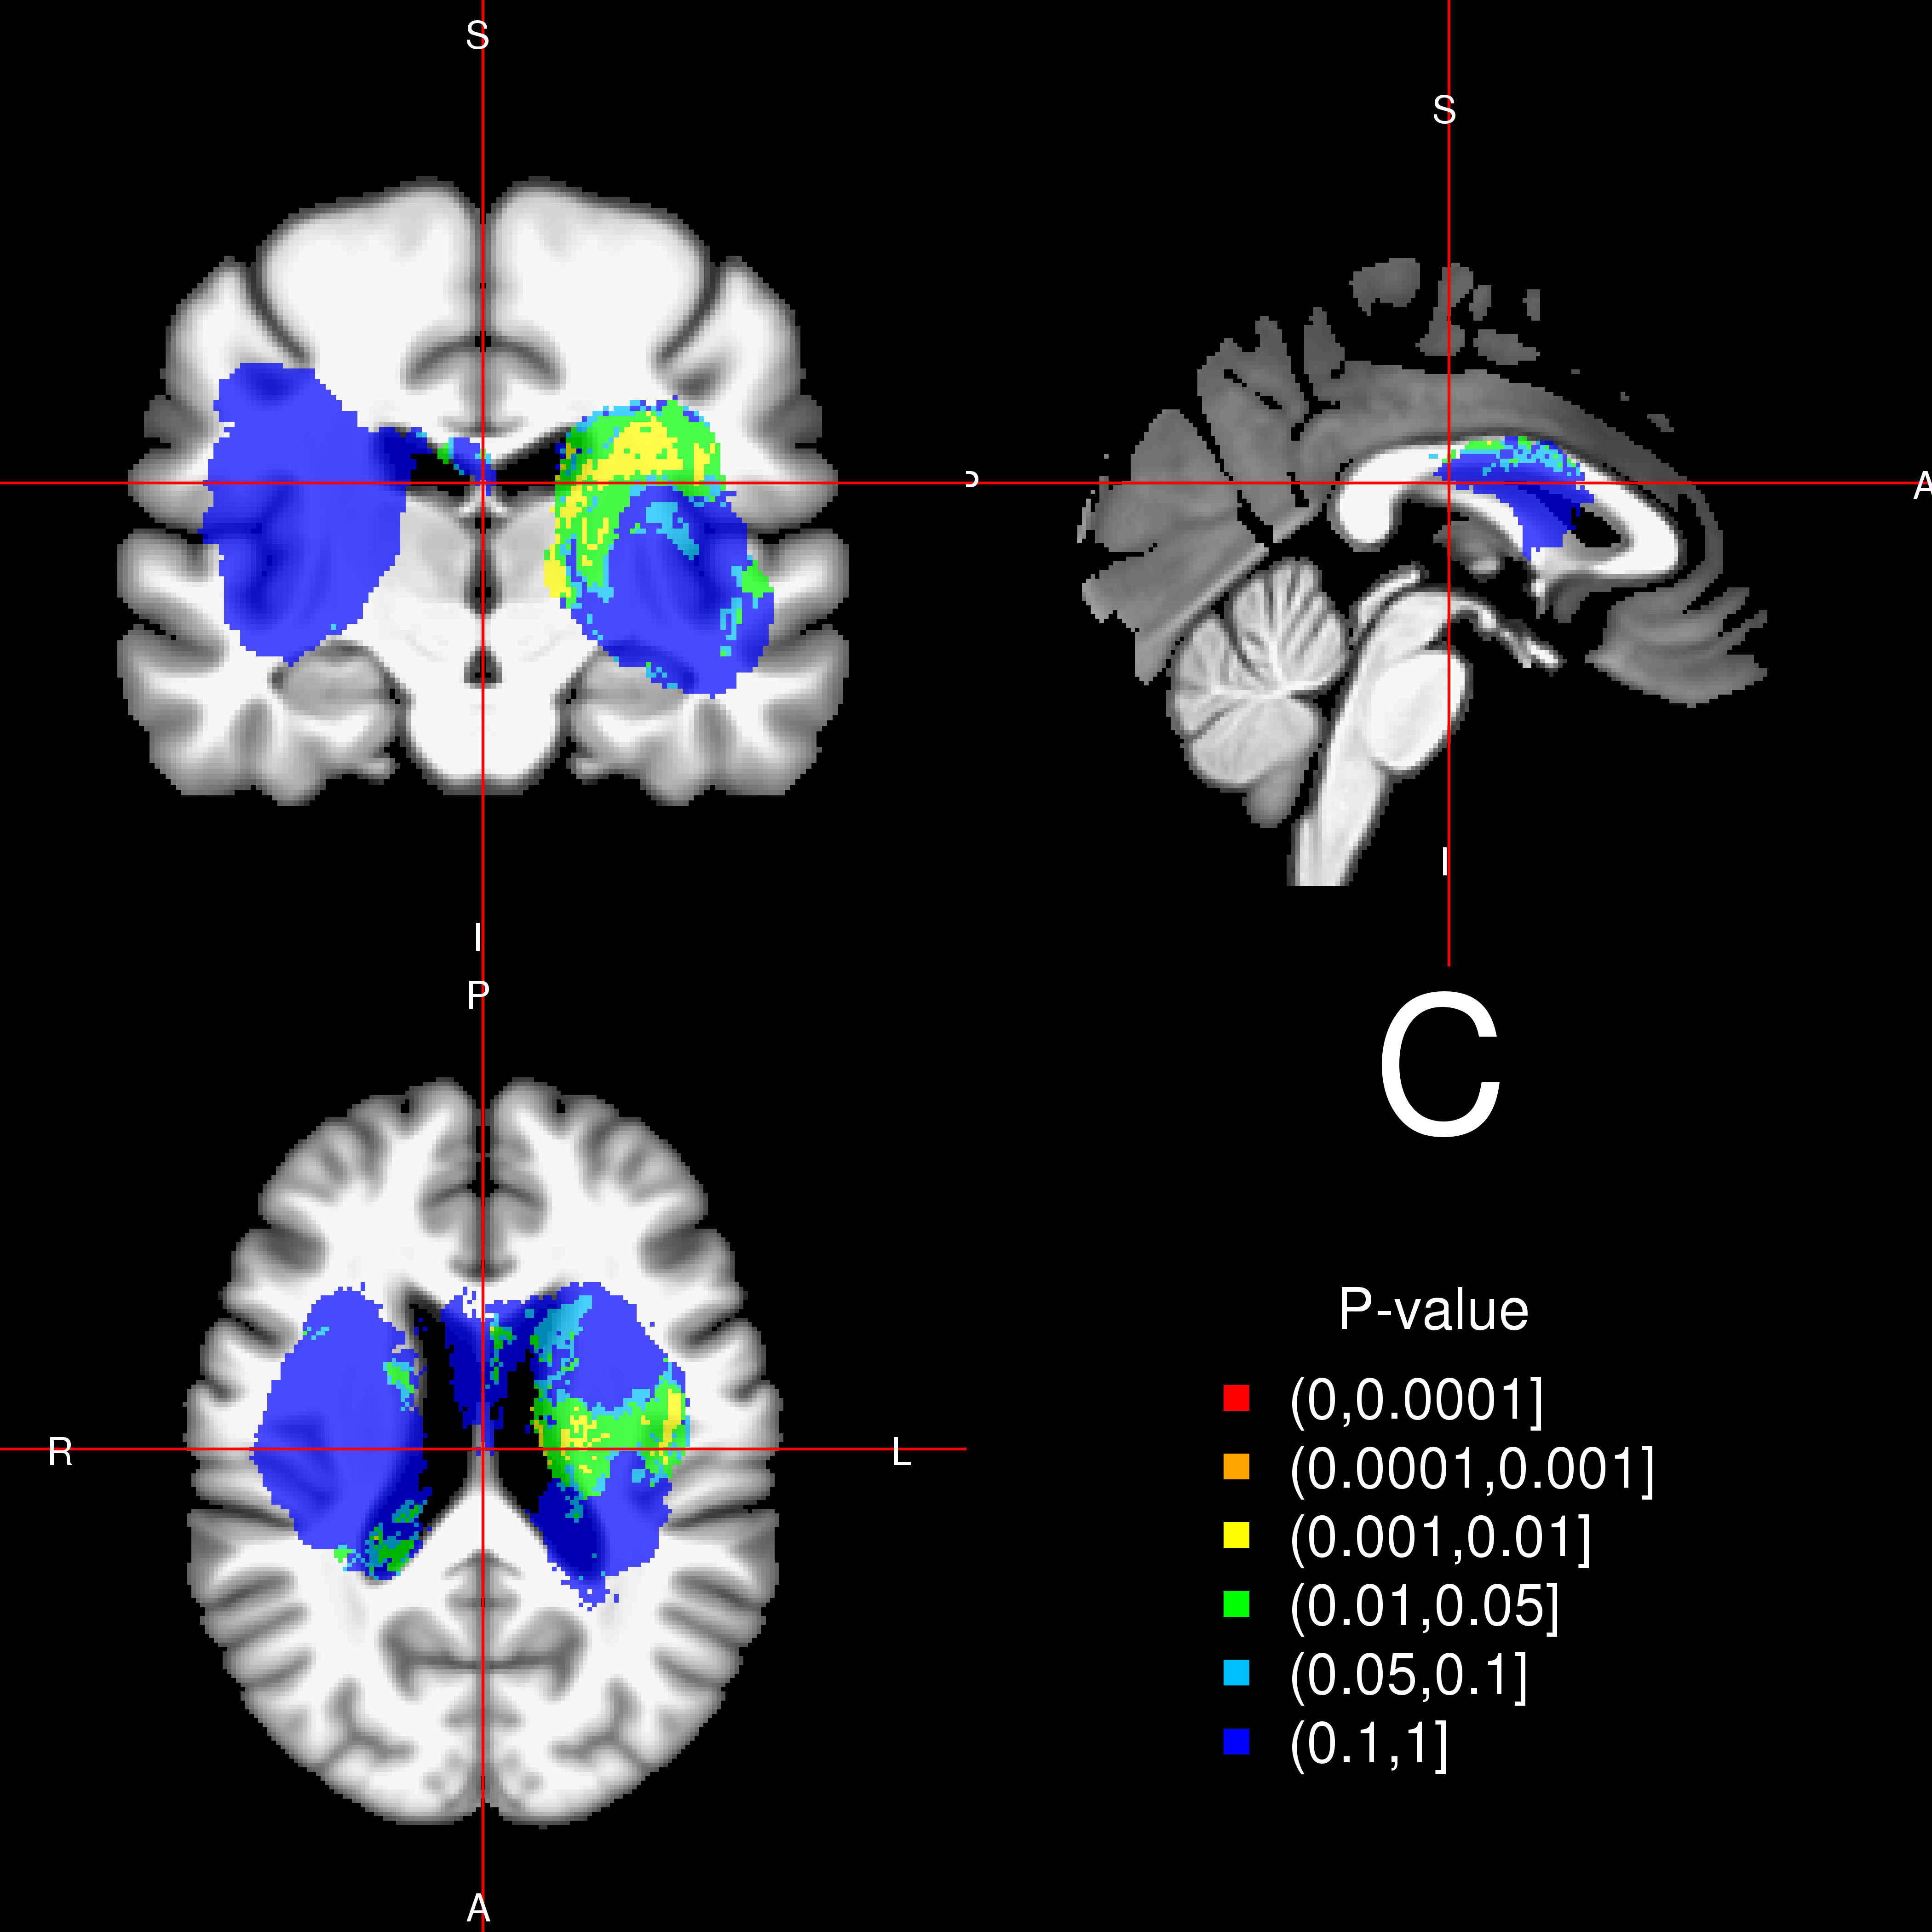
\includegraphics[width=.48\textwidth]{Regression_Map_heatcol5_t1_Final.png}
 }
  \hfill
  \subfloat{
 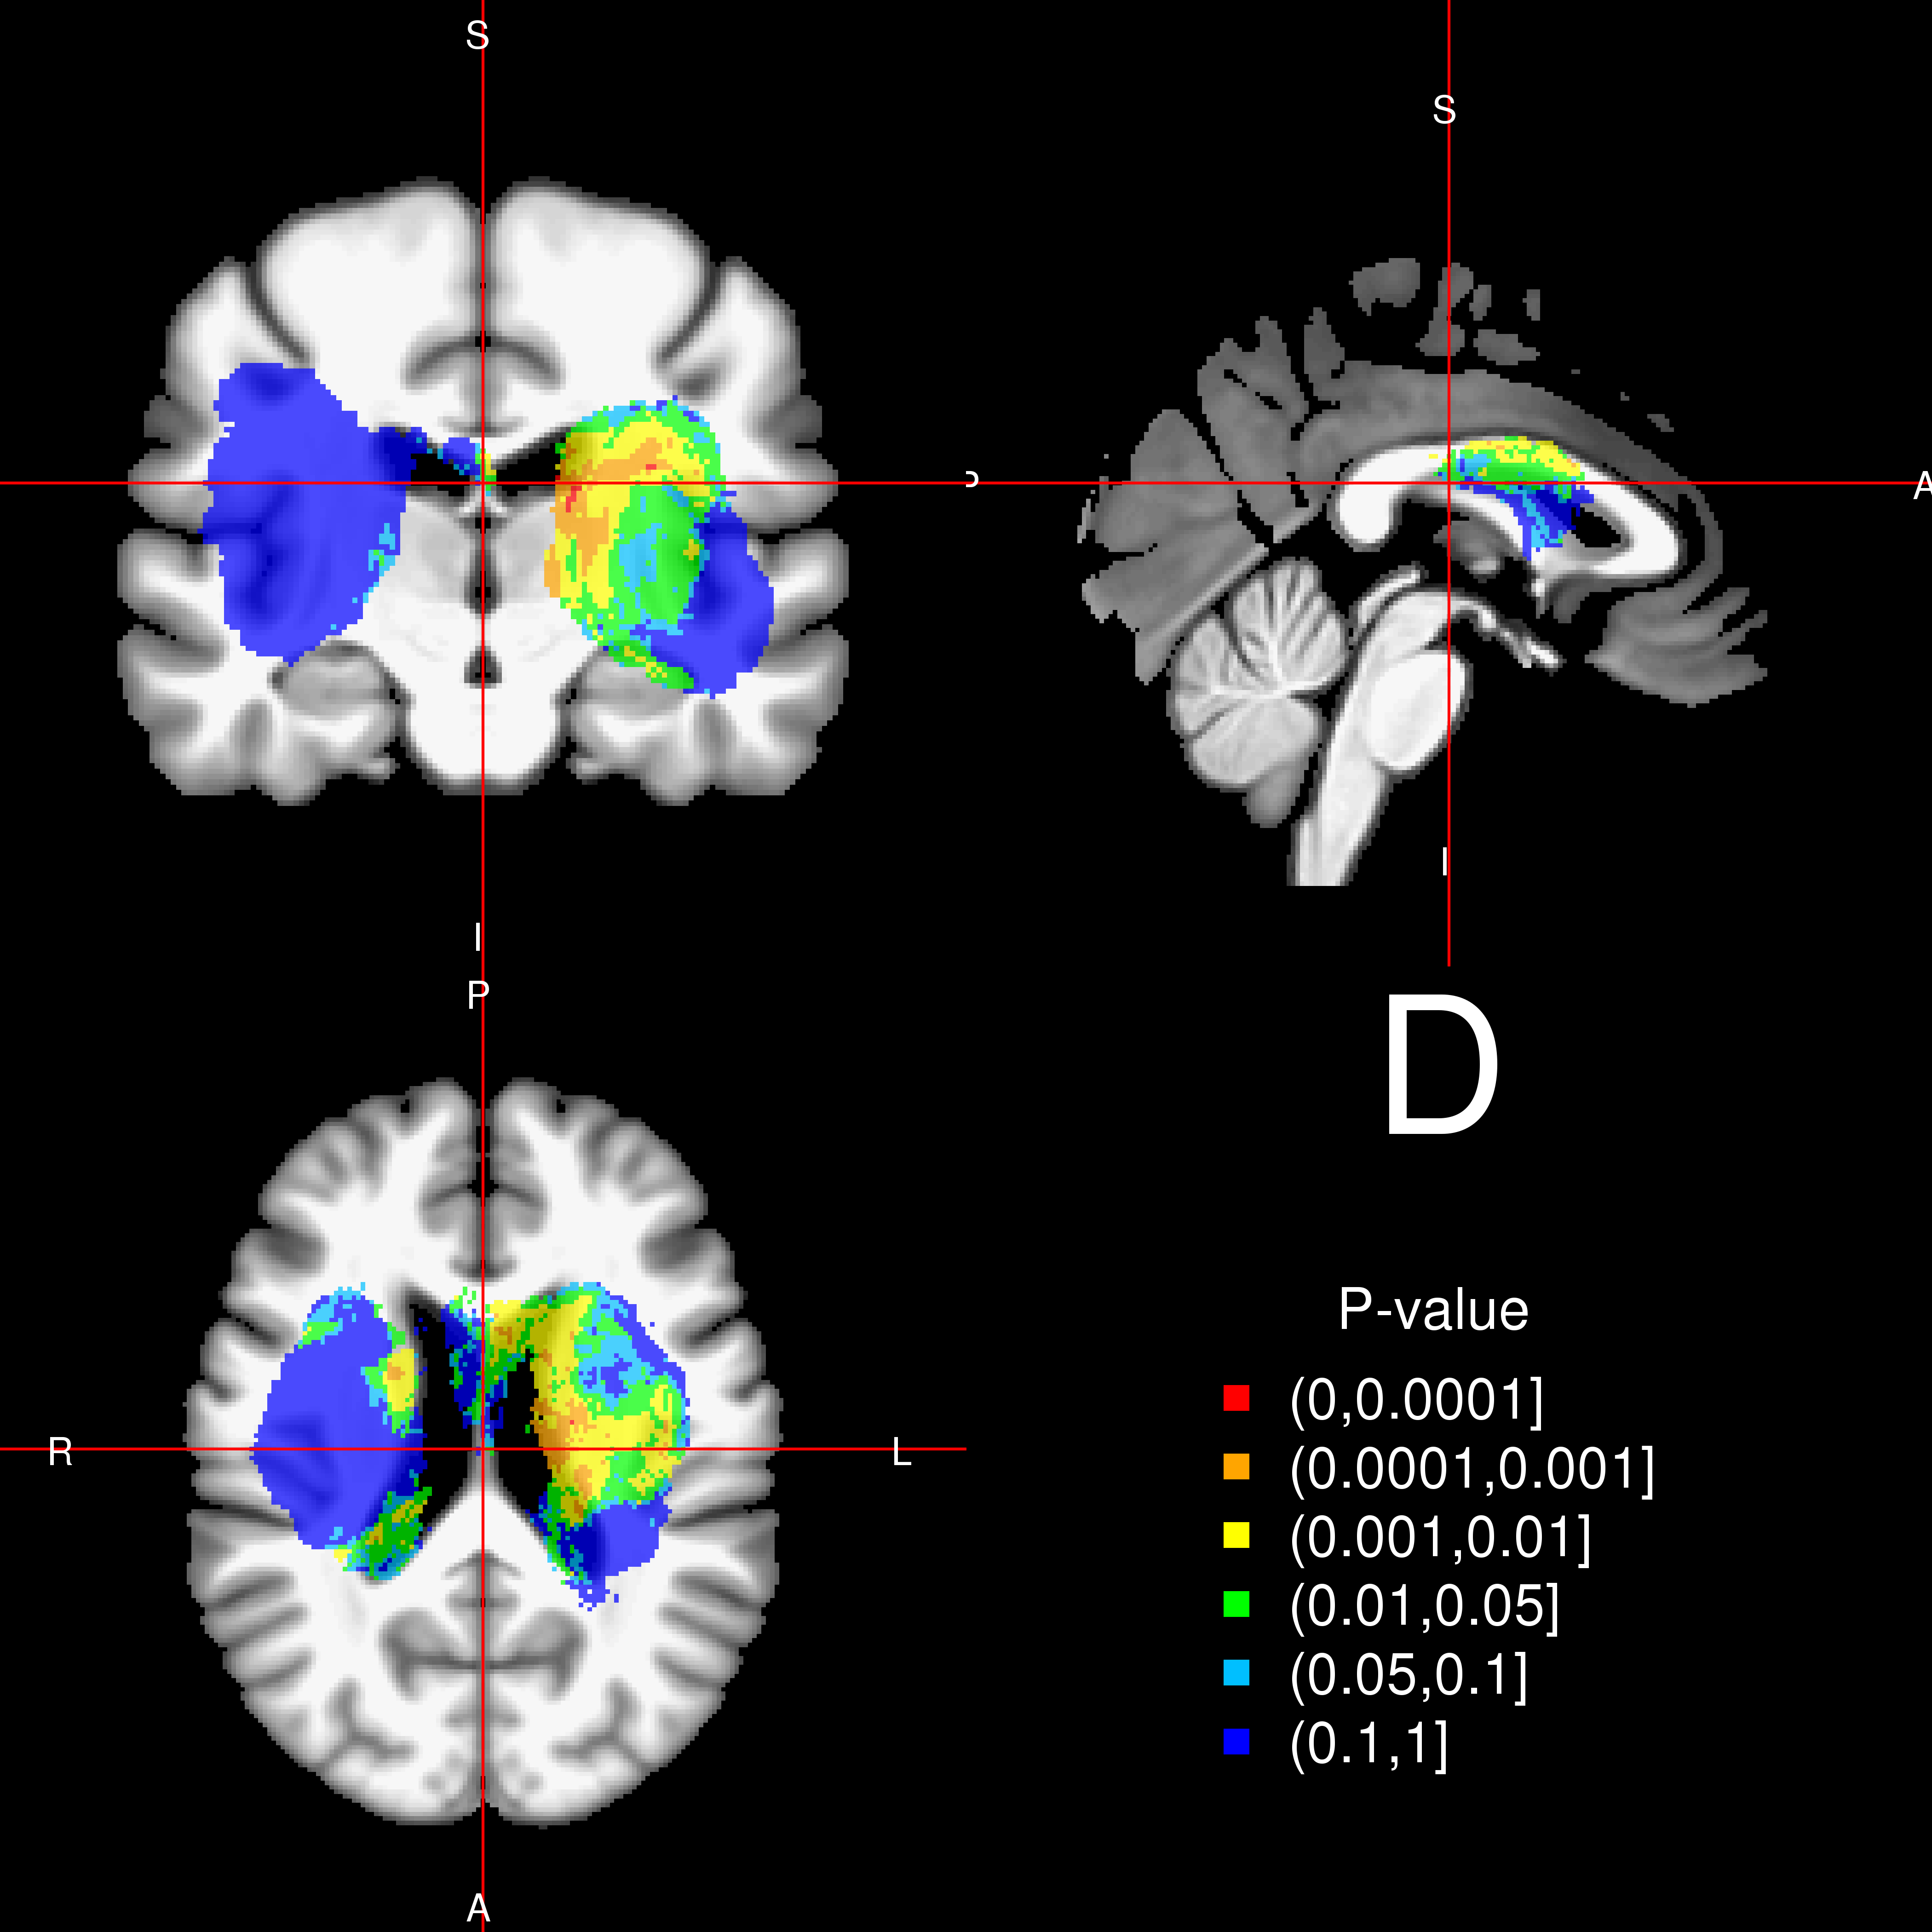
\includegraphics[width=.48\textwidth]{Regression_Map_heatcol6_t1_Final.png}
 } 
  \caption{}
\end{figure}




\begin{figure}[H]
\centering
  \hfill
  \subfloat{
 \includegraphics[width=.48\textwidth]{{Top_0.01_pvalues_Final}.png}
 }
  \hfill
  \subfloat{
 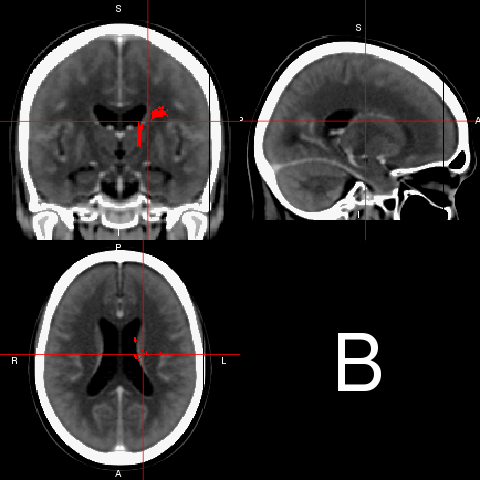
\includegraphics[width=.48\textwidth]{GCS_Top_1000_pvalues_Final.png}
 } 
 \newline
  \hfill
  \subfloat{
 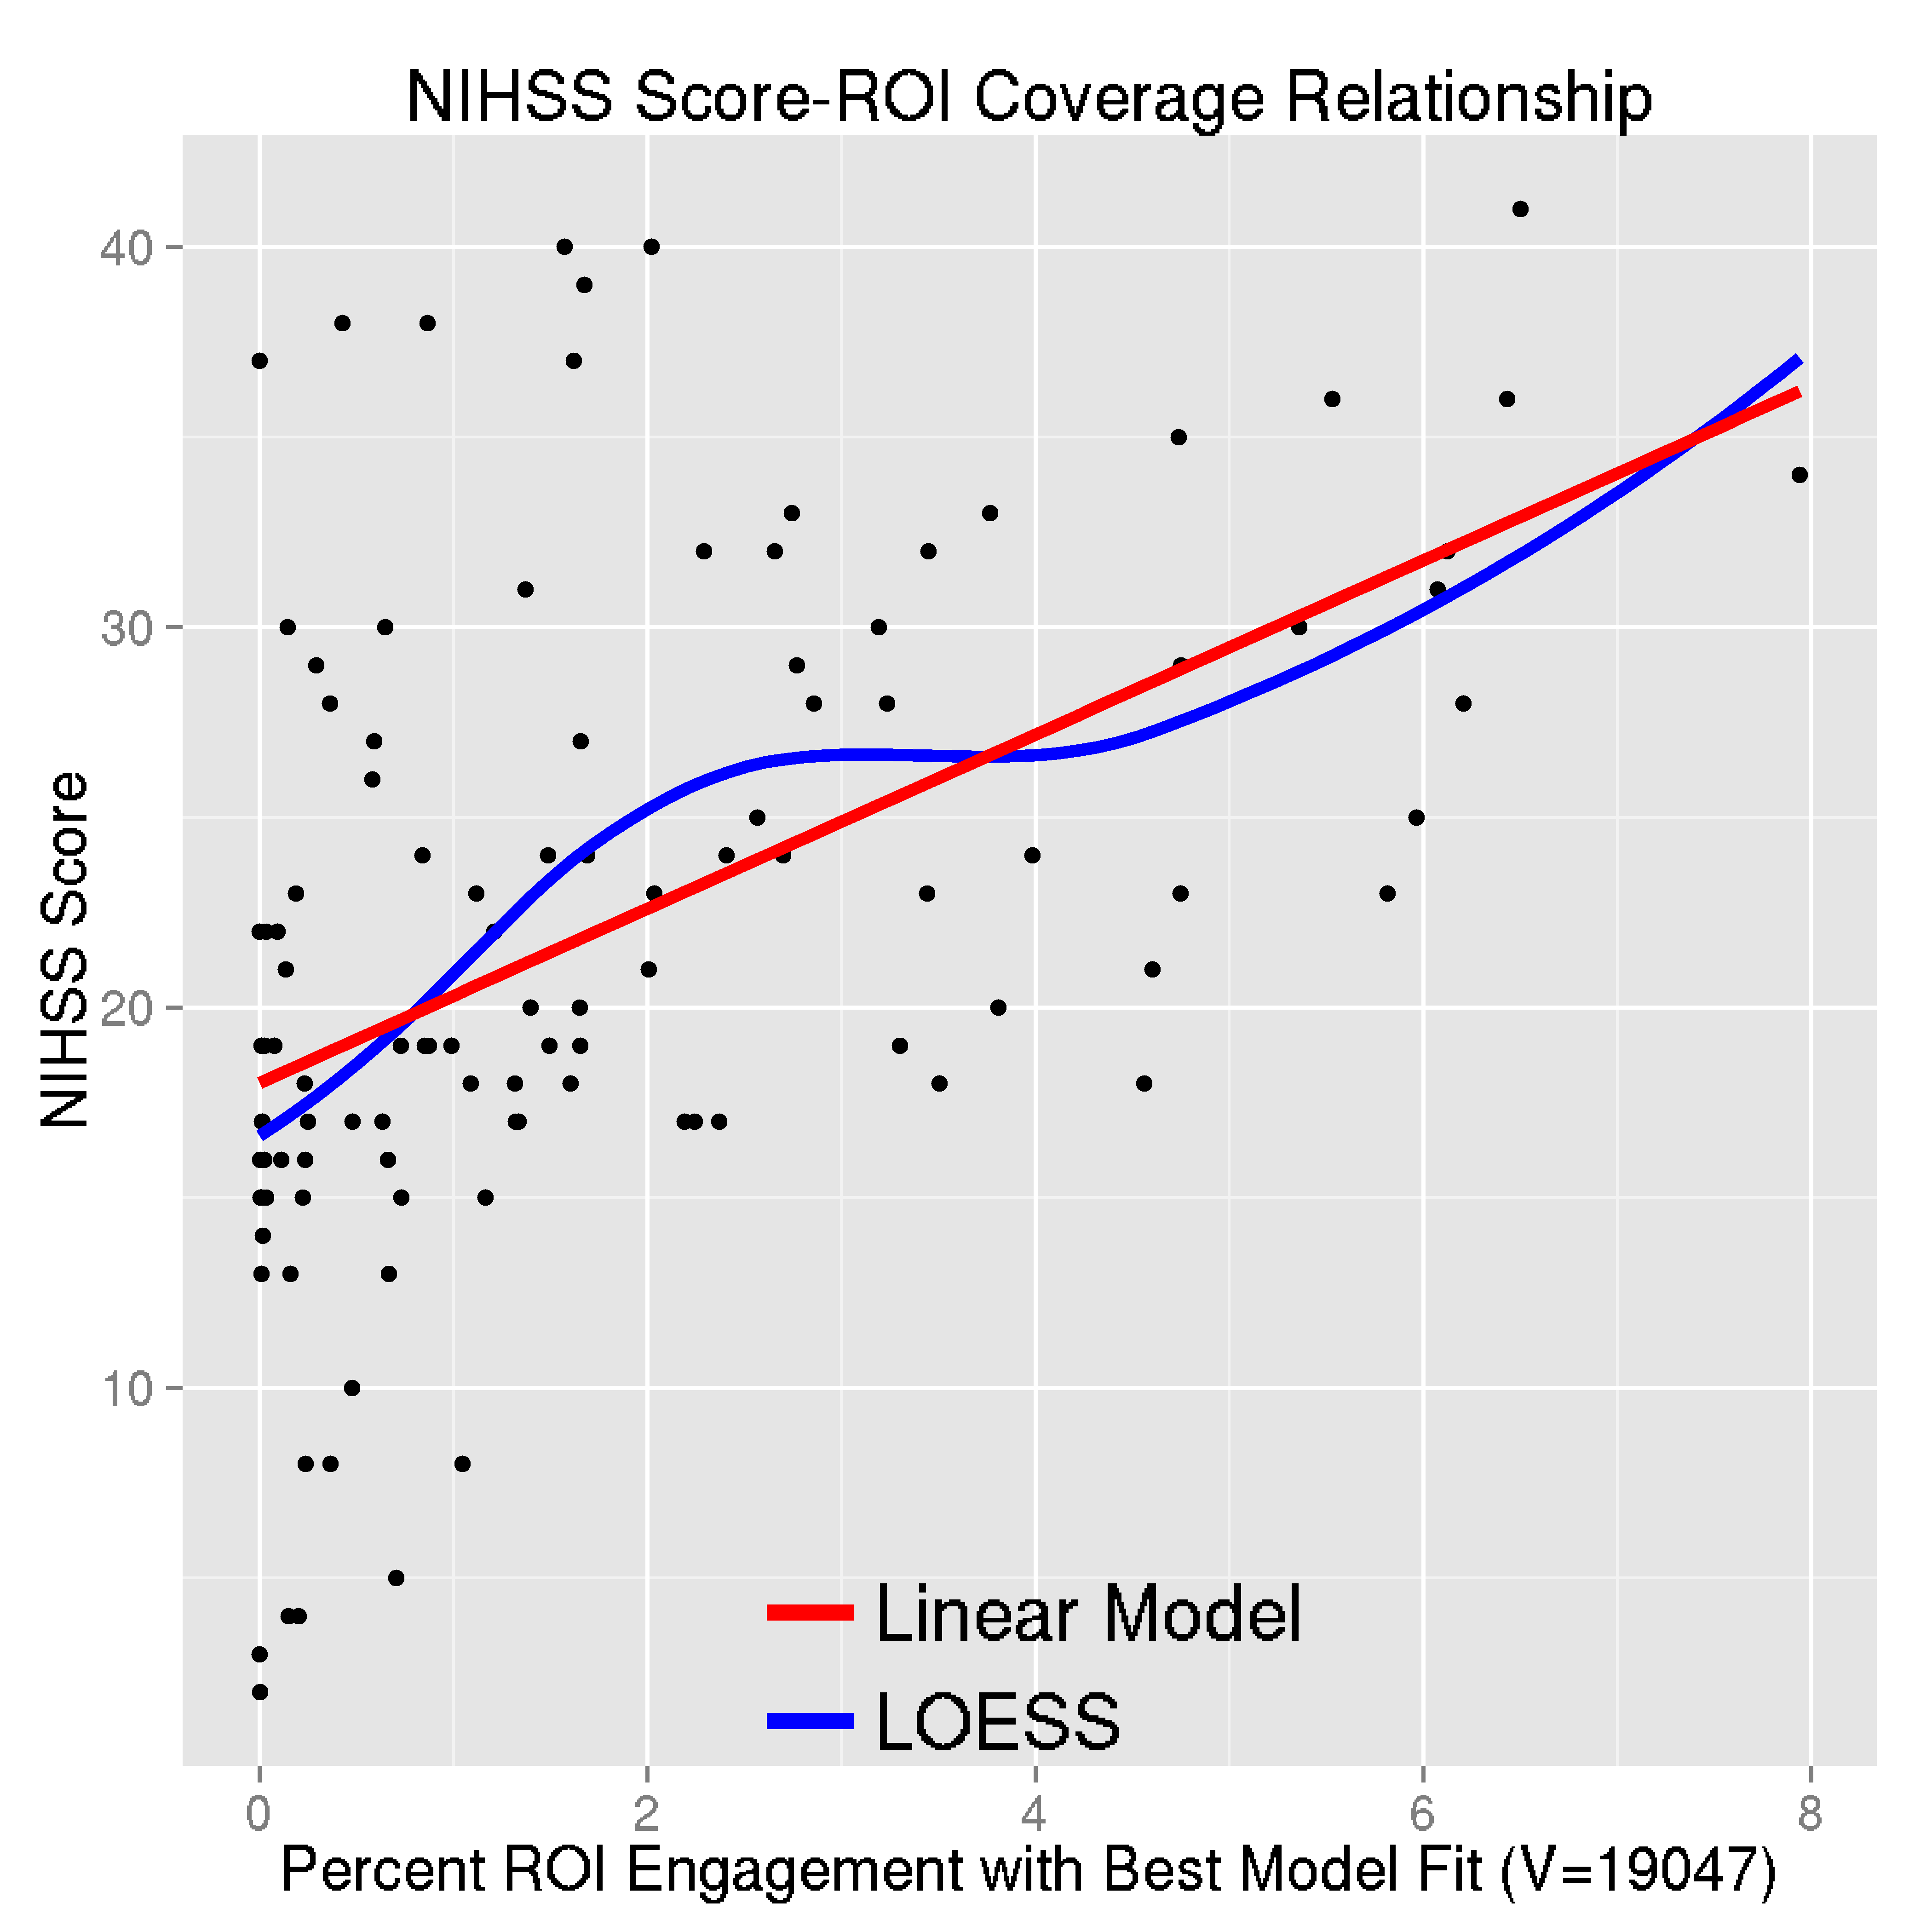
\includegraphics[width=.48\textwidth]{Regress_ROI_NIHSS_Best_Model.png}
 }
  \hfill
  \subfloat{
 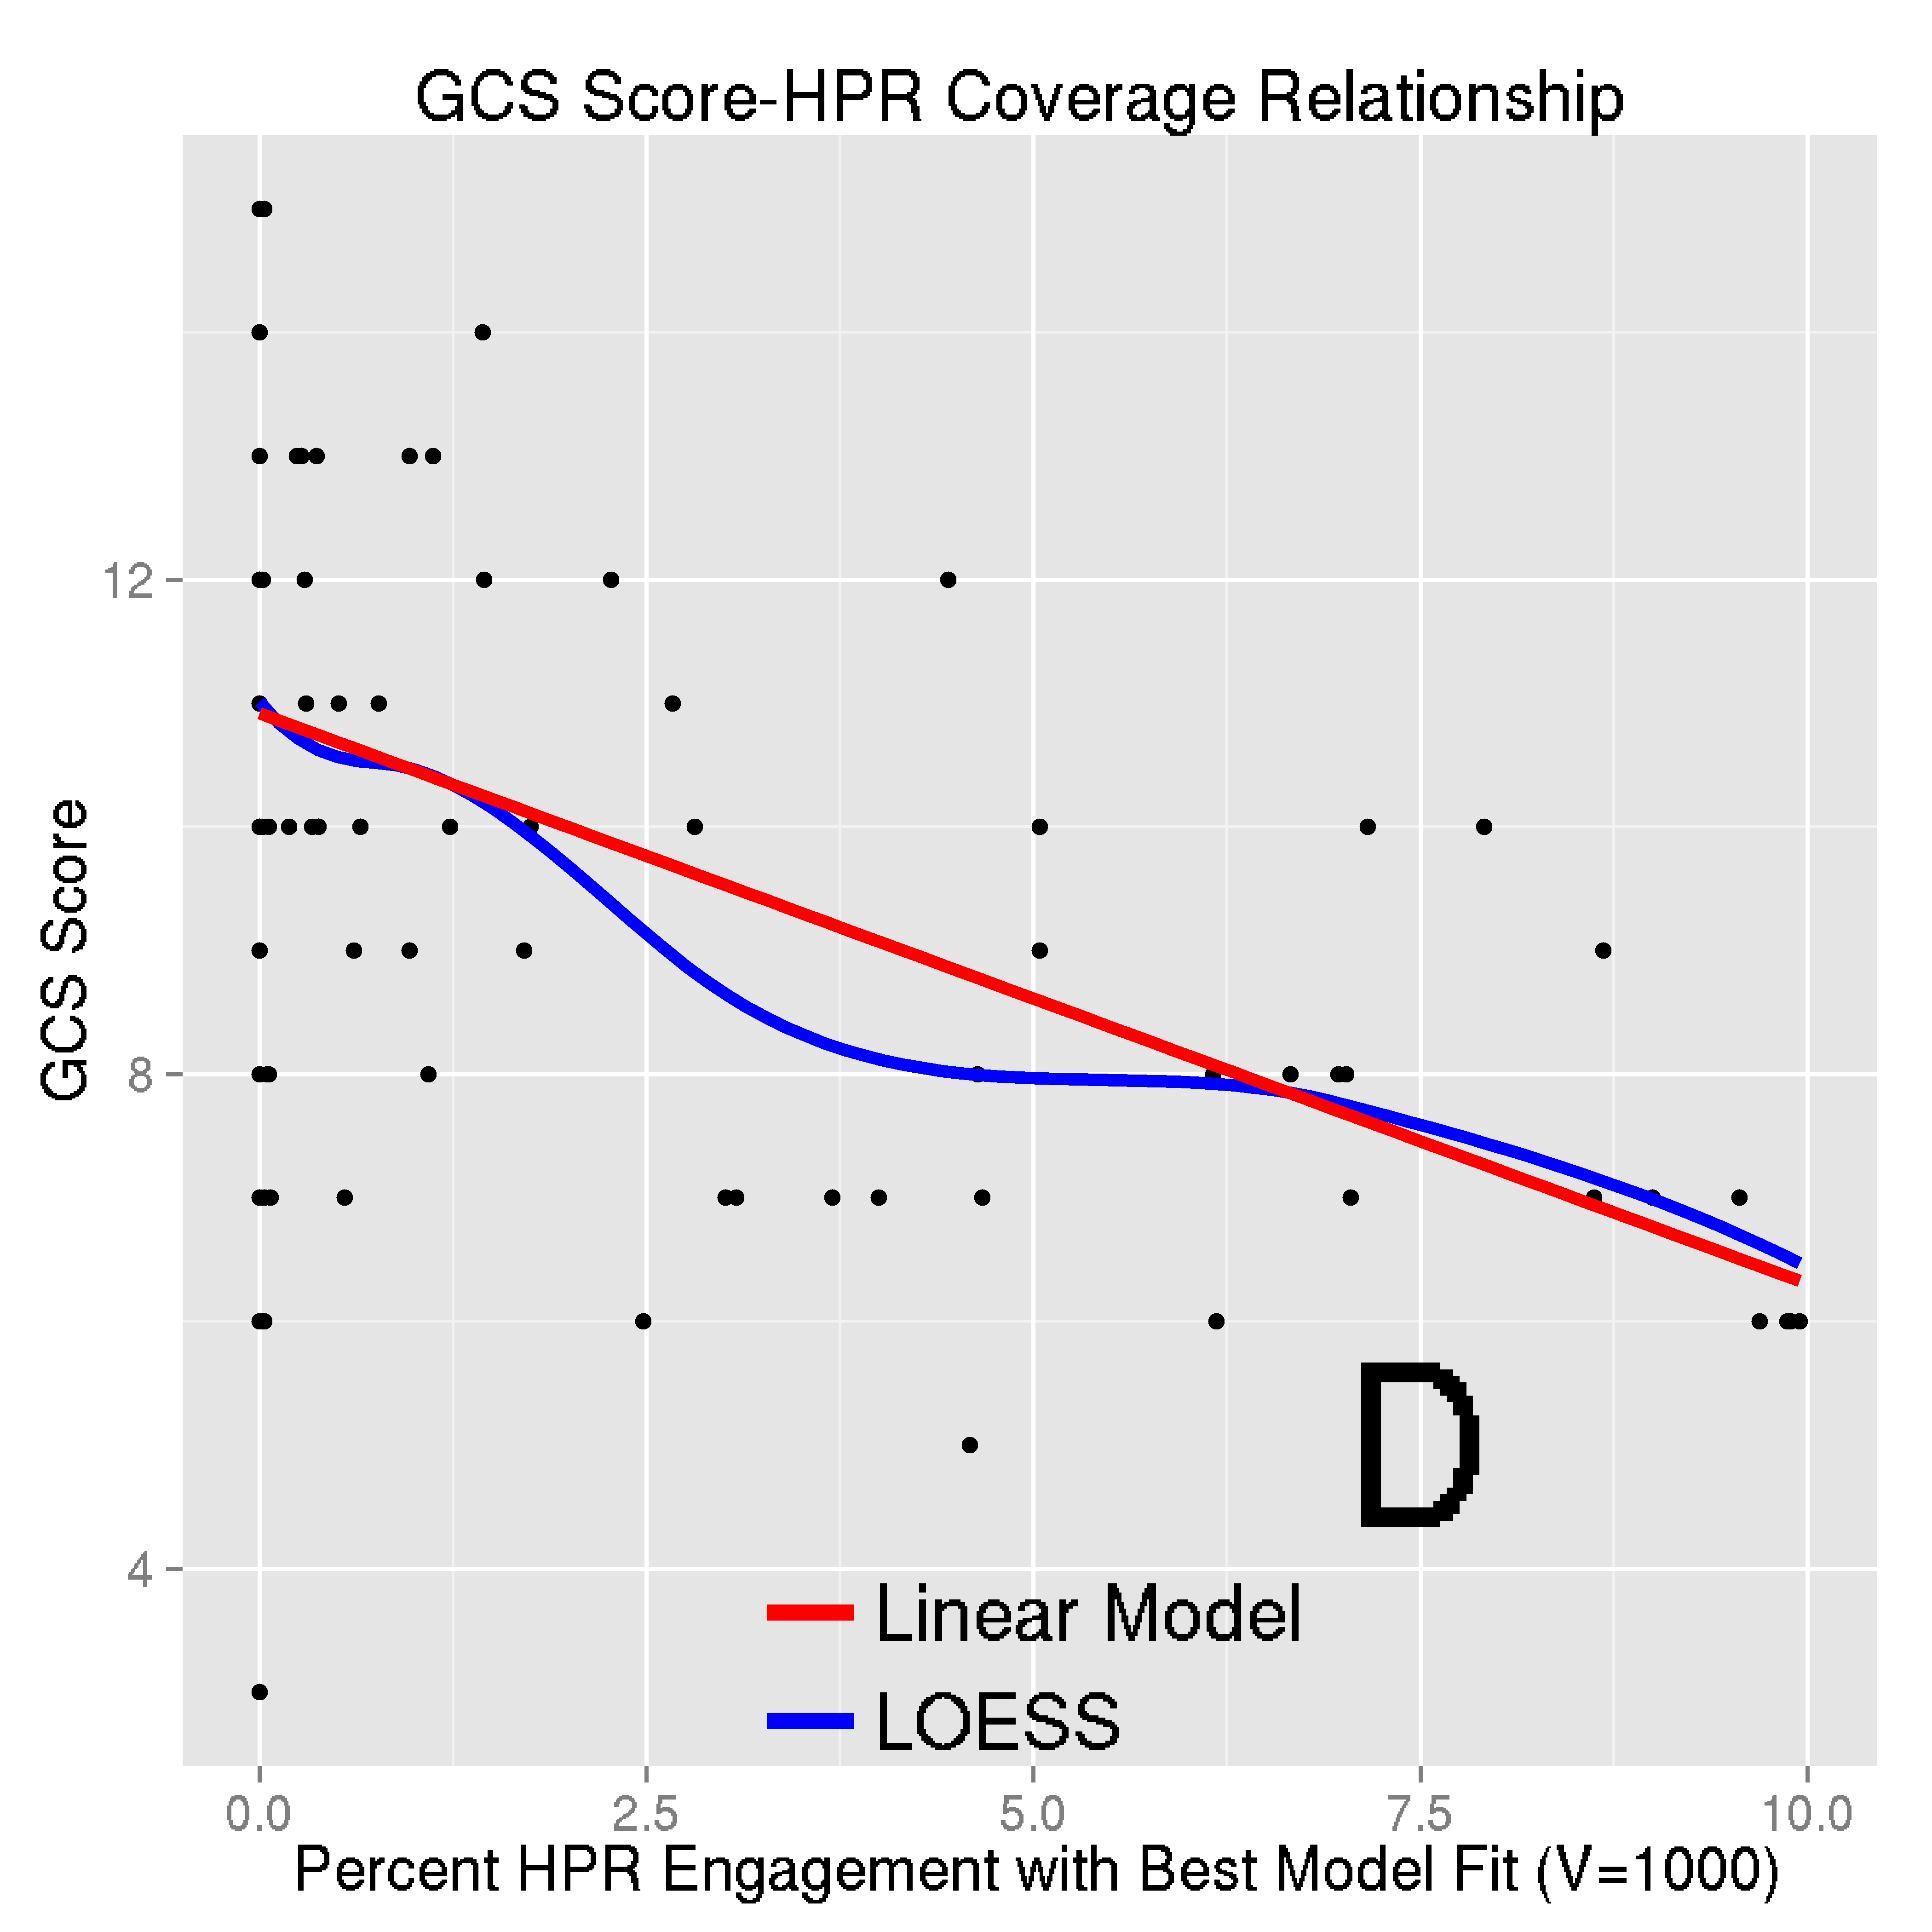
\includegraphics[width=.48\textwidth]{Regress_ROI_GCS_Best_Model.png}
 }  
 \caption{}
\end{figure}



\newpage
\setcounter{figure}{0}
\renewcommand{\thefigure}{\Roman{figure}}
\setcounter{table}{0}
\renewcommand{\thetable}{\Roman{table}}


\section{Supplemental Material}

\subsection{Supplemental Methods}
\subsubsection{Image Processing: Brain Extraction, Reorientation, Registration}
\label{sec:processing}
The hemorrhage was excluded when registering the CT scan to the template using manual ICH segmentations.  Binary ICH masks had voxels set $1$ if the voxel was hemorrhage, and $0$ otherwise.  

CT images were processed as follows:
\begin{enumerate}
\item Export from OsiriX to DICOM format
\item Gantry tilt corrected (if applicable) using MATLAB script (\url{http://bit.ly/1ltIM8c})
\item Converted to the Neuroimaging Informatics Technology Initiative (NIfTI) format using \verb|dcm2nii| (2009 version, MRIcro \citep{rorden_stereotaxic_2000})
\item Brain extraction tool (BET) \citep{smith_fast_2002}, a function of FSL (v5.0.4) \citep{jenkinson_fsl_2012} was applied
\item The data was aligned to the anterior-posterior commissure line (\url{http://bit.ly/1gUqMDw}).
\item The Clinical toolbox \citep{rorden_age-specific_2012} was applied.
\end{enumerate}
 An image with its brain-extracted counterpart is displayed in Supplemental Figure~\ref{f:reg}\protect\subref*{reg:ss1}.

We thresholded the smoothed hemorrhage mask: let $S_i$ be the smoothed mask for person $i$, and $s_{ij}$ be voxel $j$ of that mask; let $v_{ij}$ represents voxel $j$ of the thresholded image.  The was thresholded using the rule \citep{rorden_age-specific_2012}:
$$
v_{ij} =
\begin{cases}
1  & \text{if } s_{ij} \geq \frac{\min(S_i) + \max(S_i)}{2}\\
0  & \text{if } s_{ij} < \frac{\min(S_i) + \max(S_i)}{2}
\end{cases}
$$
These binary ICH masks were used in analysis.  

\subsubsection{Calculating Region Engagement from the Eve Atlas}
\label{sec:calc_perc}
We also calculated the percent engagement of regions for the best-performing HPR for the NIHSS and GCS score analyses.
More explicitly, let $k$ denote the brain region (e.g. Putamen) and let $\sum_{k} v_{k}$ represent the sum of the voxels for an image (HPR or population ICH image) in that brain region. These $p_{k}$ represent the percent that brain region engages the ICH compared to other regions (Table~\ref{t:breakdown}):
$$
  p_{k} = \frac{\sum_{k} v_{k}}{\text{Sum of Image}}
$$
We also calculated brain region engagement with the population ICH or HPR images (Table~\ref{t:area_breakdown}):
$$
	r_{k} = \frac{\sum_{k} v_{k}}{\# \text{Number of Voxels in Region}}
$$
These percentages ($r_{k}$) are at a region level; $p_k$ are at an image level.



\subsubsection{Image Registration}


We present the registration results (Figure~\ref{f:reg}):  manually segmented blood in the original space with the hemorrhage mask in pink (panel~\protect\subref*{reg:nat1}), brain-extracted image (panel~\protect\subref*{reg:ss1}), registered image and hemorrhage mask in template space (panel~\protect\subref*{reg:co1}), and the ICH mask on the template (panel~\protect\subref*{reg:temp1}).  These images represent one patient with variable slice thickness with a large hemorrhage.

Though variable slice thickness is present, the transformation morphs the image into the full space of the template; therefore, non-linear registration seems to reasonably account for variable slice thickness, likely by non-uniform scaling.
We also see gross brain features remain relatively unchanged, but large deformations of tissue, due to ICH, appear well preserved by registration.  

[Figure~\ref{f:reg} here.]



\newpage

\subsection{Supplemental Tables}

% Table created by stargazer v.5.0 by Marek Hlavac, Harvard University. E-mail: hlavac at fas.harvard.edu
% Date and time: Fri, May 16, 2014 - 02:31:21
\begin{table}[!htbp] \centering 
\begin{tabular}{@{\extracolsep{5pt}}lcccc} 
\\[-1.8ex]\hline 
\\[-1.8ex] & \multicolumn{2}{c}{\textbf{NIHSS Score}} & \multicolumn{2}{c}{\textbf{GCS Score}} \\ 
 & \textbf{ROI Coverage} & \textbf{Reader-Location} & \textbf{ROI Coverage} & \textbf{Reader-Location} \\ 
\hline \\[-1.8ex] 
 Age & $-$0.04 ($-$0.2, 0.1) & $-$0.1 ($-$0.2, 0.1) & 0.02 ($-$0.03, 0.1) & 0.02 ($-$0.03, 0.1) \\ 
  Sex: Male vs. Female & $-$0.7 ($-$3.8, 2.4) & $-$1.7 ($-$5.0, 1.7) & 0.03 ($-$1.1, 1.1) & 0.1 ($-$1.1, 1.3) \\ 
  TICHVol per 10 cc & 0.8$^{}$ ($-$0.003, 1.5) & 1.6$^{}$ (0.8, 2.4) & $-$0.2$^{}$ ($-$0.5, 0.02) & $-$0.5$^{}$ ($-$0.7, $-$0.2) \\ 
  ROI Coverage per 10\% & 2.0$^{}$ (1.1, 2.8) &  & $-$0.4$^{}$ ($-$0.6, $-$0.2) &  \\ 
  Reader-Based Location&&&& \\
\;\;Globus Pallidus &  & 4.5 ($-$2.9, 11.9) &  & $-$1.8 ($-$4.5, 0.8) \\ 
  \;\;Putamen &  & 4.2$^{}$ (0.3, 8.2) &  & $-$1.2$^{}$ ($-$2.6, 0.2) \\ 
  \;\;Thalamus &  & 4.8 ($-$4.1, 13.6) &  & $-$1.0 ($-$4.2, 2.1) \\ 
  Constant & 18.8$^{}$ (9.1, 28.4) & 19.6$^{}$ (7.5, 31.7) & 10.6$^{}$ (7.4, 13.7) & 11.2$^{}$ (6.9, 15.5) \\ 
\hline 
\end{tabular} 
  \caption{Regression Models for ROI-Based Analysis. The models for ROI coverage represent the best model based on the model-fit measures. We see that after adjusting for age, sex, and total baseline ICH volume, increasing 10\% coverage is expected to increase NIHSS score by 2.0 (95\% CI: 1.1, 2.8) points.  We see that all locations, compared to lobar hemorrhages have higher estimated NIHSS scores, but putaminal hemorrhages were significantly higher by 4.2 (95\% CI: 0.2, 8.2) points. Adjusting for other covariates, increasing 10\% coverage is expected to decrease GCS score by 0.4 (95\% CI: 0.6, 0.2) points.  We see that all locations, compared to lobar hemorrhages have lower estimated GCS scores, but none were statistically different.} 
  \label{f:beta} 
\end{table} 


% latex table generated in R 3.1.0 by xtable 1.7-3 package
% Tue Jul 15 14:35:49 2014
\begin{table}[ht]
\centering
\begin{tabular}{lccc}
  \hline
Area & Population Engagement & NIHSS HPR & GCS HPR \\ 
  \hline
Globus Pallidus: Total & 20.3 & 40.0 & 0.0 \\ 
  Globus Pallidus: Right & 14.8 & 34.8 & 0.0 \\ 
  Globus Pallidus: Left & 25.2 & 44.7 & 0.0 \\ 
  Putamen: Total & 23.3 & 6.6 & 0.0 \\ 
  Putamen: Right & 17.5 & 3.8 & 0.0 \\ 
  Putamen: Left & 29.2 & 9.4 & 0.0 \\ 
  Thalamus: Total & 7.9 & 8.9 & 1.7 \\ 
  Thalamus: Right & 6.8 & 3.1 & 0.0 \\ 
  Thalamus: Left & 9.1 & 14.6 & 3.4 \\ 
   \hline
\end{tabular}
\caption{Engagement of the Thalamus, Putamen and Globus Pallidus by the population  3D histogram, the NIHSS HPR based on a p-value  threshold of $.01$, the GCS HPR based on voxels with $1000$ smallest p-values.  Each distribution  is based on the Eve atlas.  The population engagement represents the mean proportion of engagement for that brain region over all patient ICH masks.  The HPR columns represent the percent of voxels in that brain region that  are in the HPR for NIHSS and GCS scores.   On average, $23\%$ of the Putamen, $20\%$ of the Globus Pallidus, and $8\%$ of the Thalmus are  engaged with ICH from patients in this study.  The HPR from the NIHSS analysis engages $40\%$ of the Globus Pallidus, $6\%$ of the Putamen, and $9\%$ of the Thalamus.  The HPR from the GCS analysis engages only $2\%$ of the Thalamus, but not the Putamen nor the Globus Pallidus; the GCS HPR is only $1000$ voxels.  All engagement is higher on the left side compared to the right. The Eveatlas can be used to calculate area engagement on a per-scan level as well to give, for example, putaminal engagement with ICH at a scan level. } 
\label{t:area_breakdown}
\end{table}




\subsection{Supplemental Figures and Figure Legends}


\begin{figure}[H]
\centering
 \subfloat{
 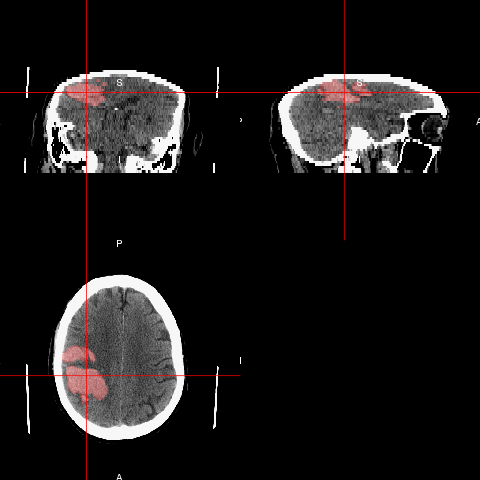
\includegraphics[width=.48\textwidth]{native_100-362_20100126_1926_CT_2_CT_ROUTINE.png}
 \label{reg:nat1}
 }
 \hfill
 \subfloat{
% \includegraphics[width=.48\textwidth]{{100-362_20100126_1926_CT_2_CT_ROUTINE_SS_0.01}.png}
 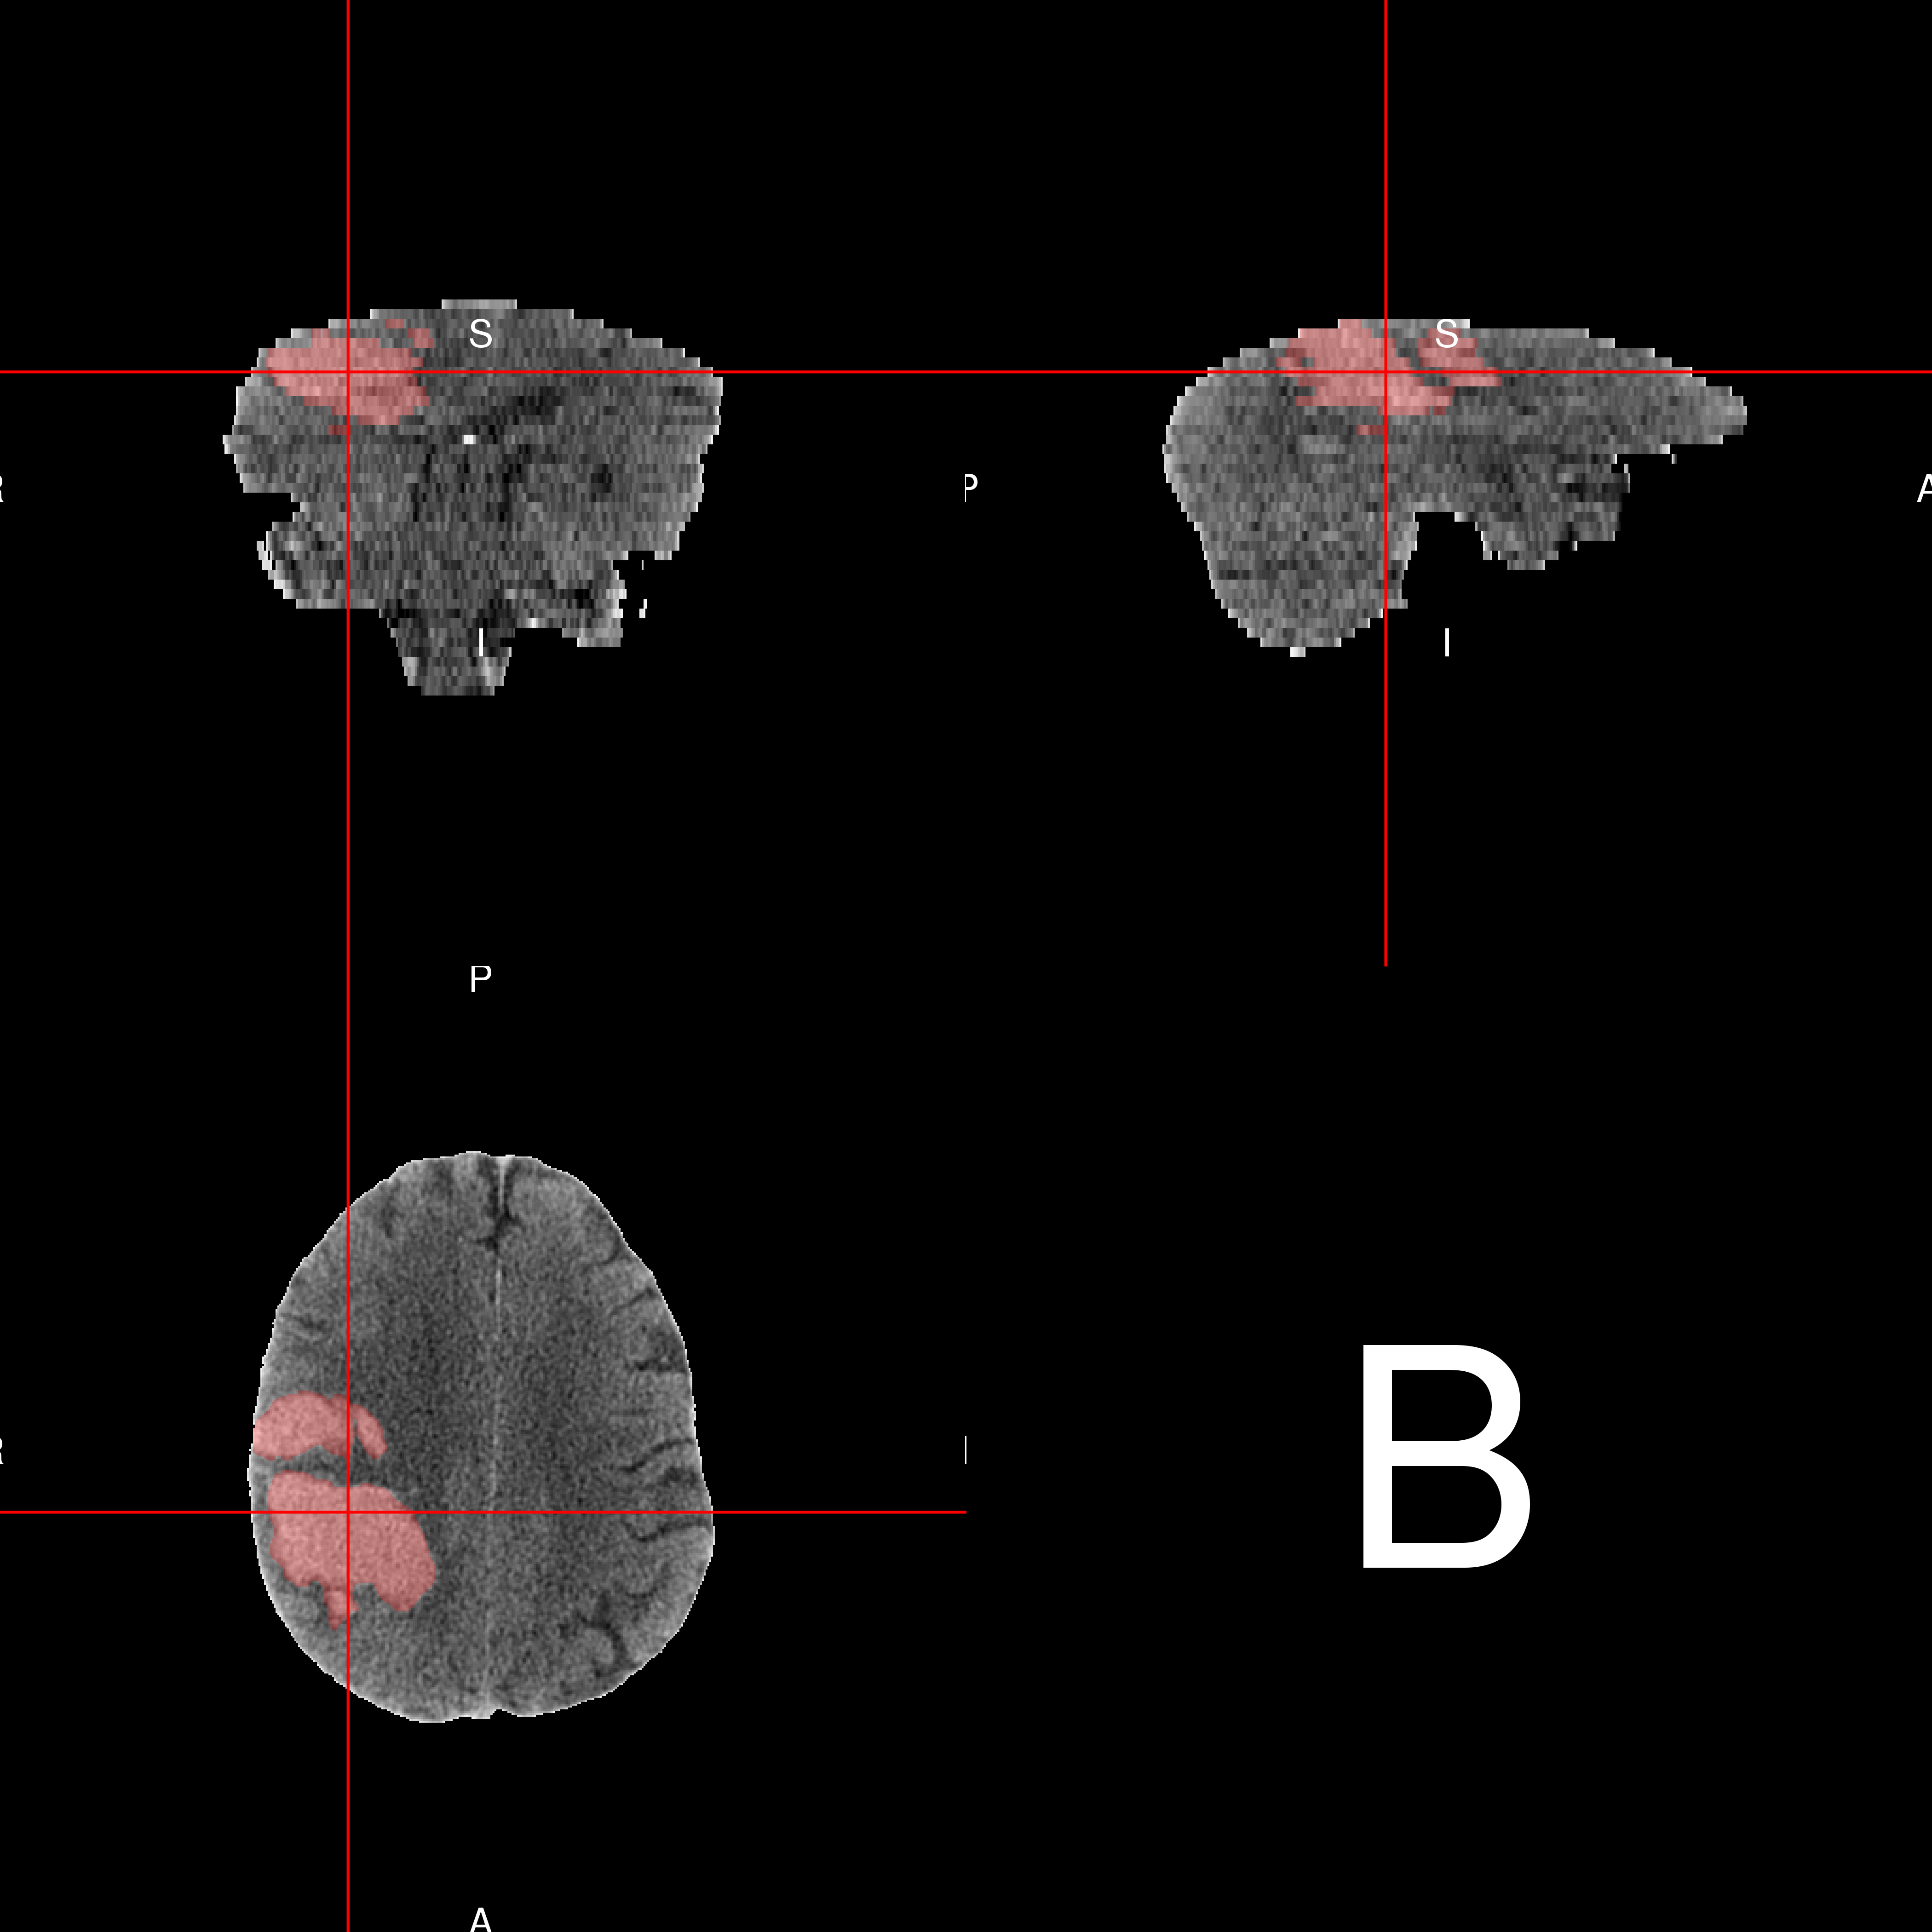
\includegraphics[width=.48\textwidth]{ss_100-362_20100126_1926_CT_2_CT_ROUTINE.png}
 \label{reg:ss1}
} 
\newline
 \subfloat{
 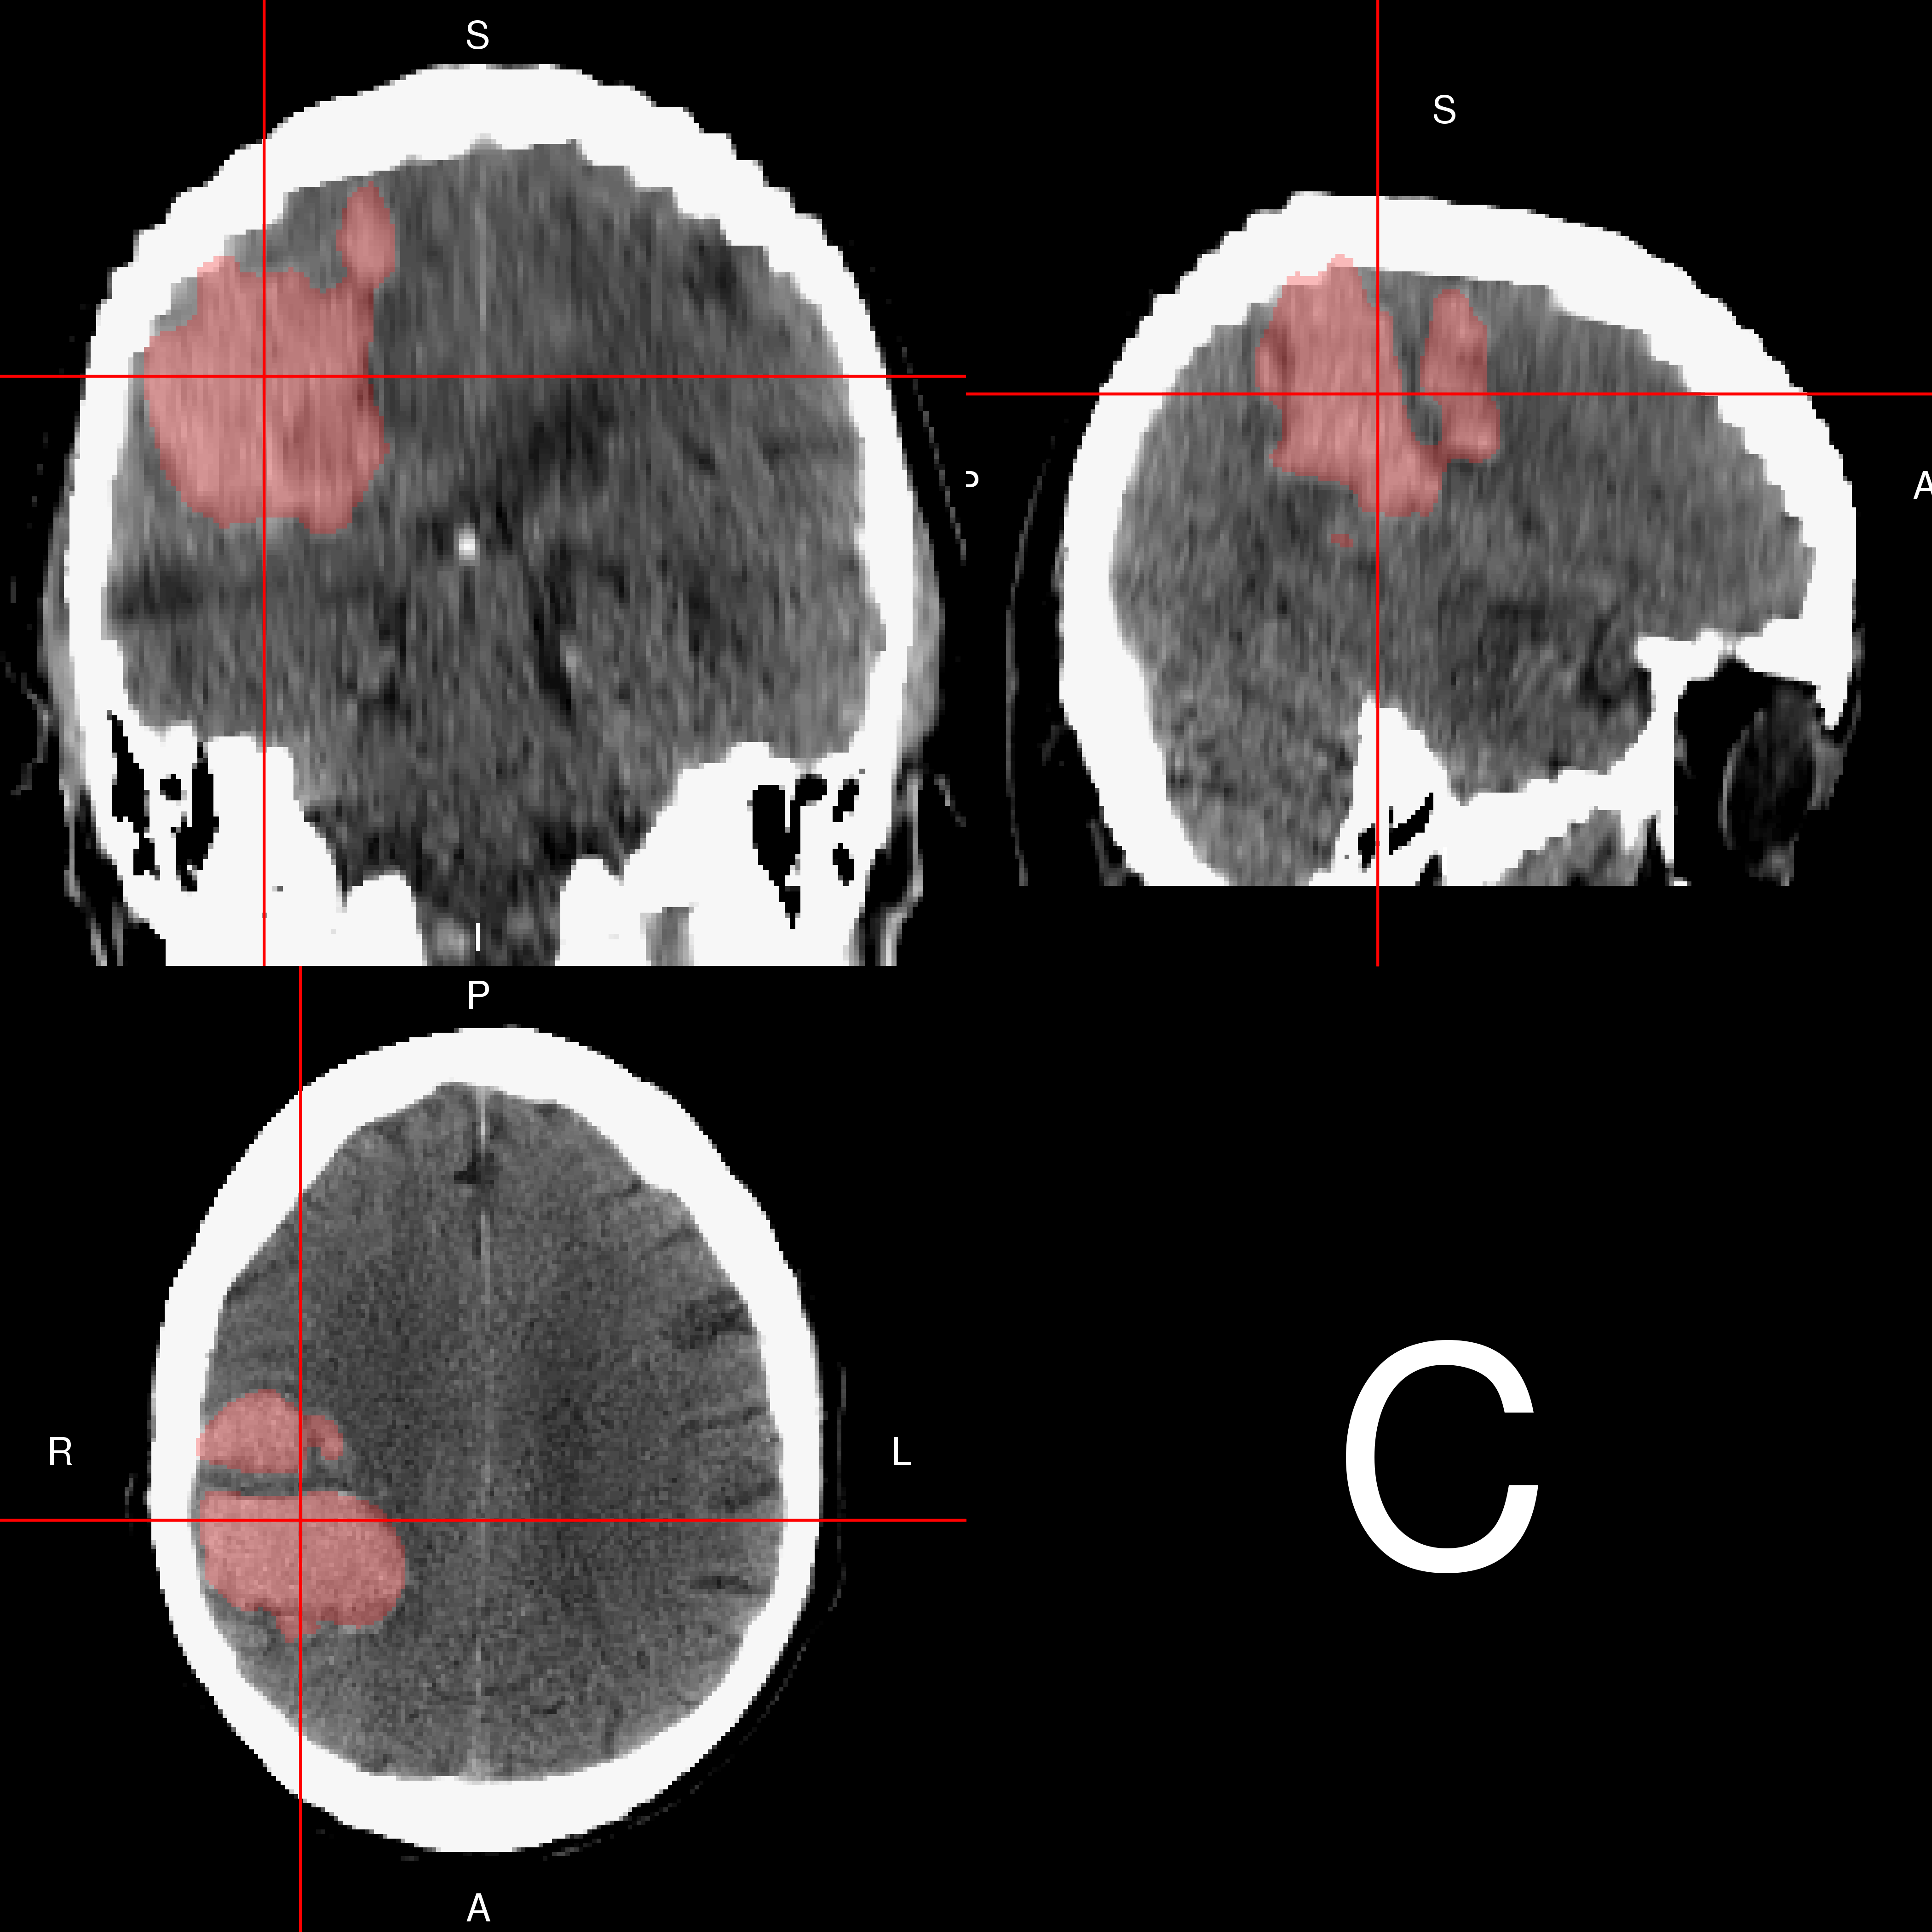
\includegraphics[width=.48\textwidth]{raw_100-362_20100126_1926_CT_2_CT_ROUTINE.png}
 \label{reg:co1}
}
  \hfill
  \subfloat{
 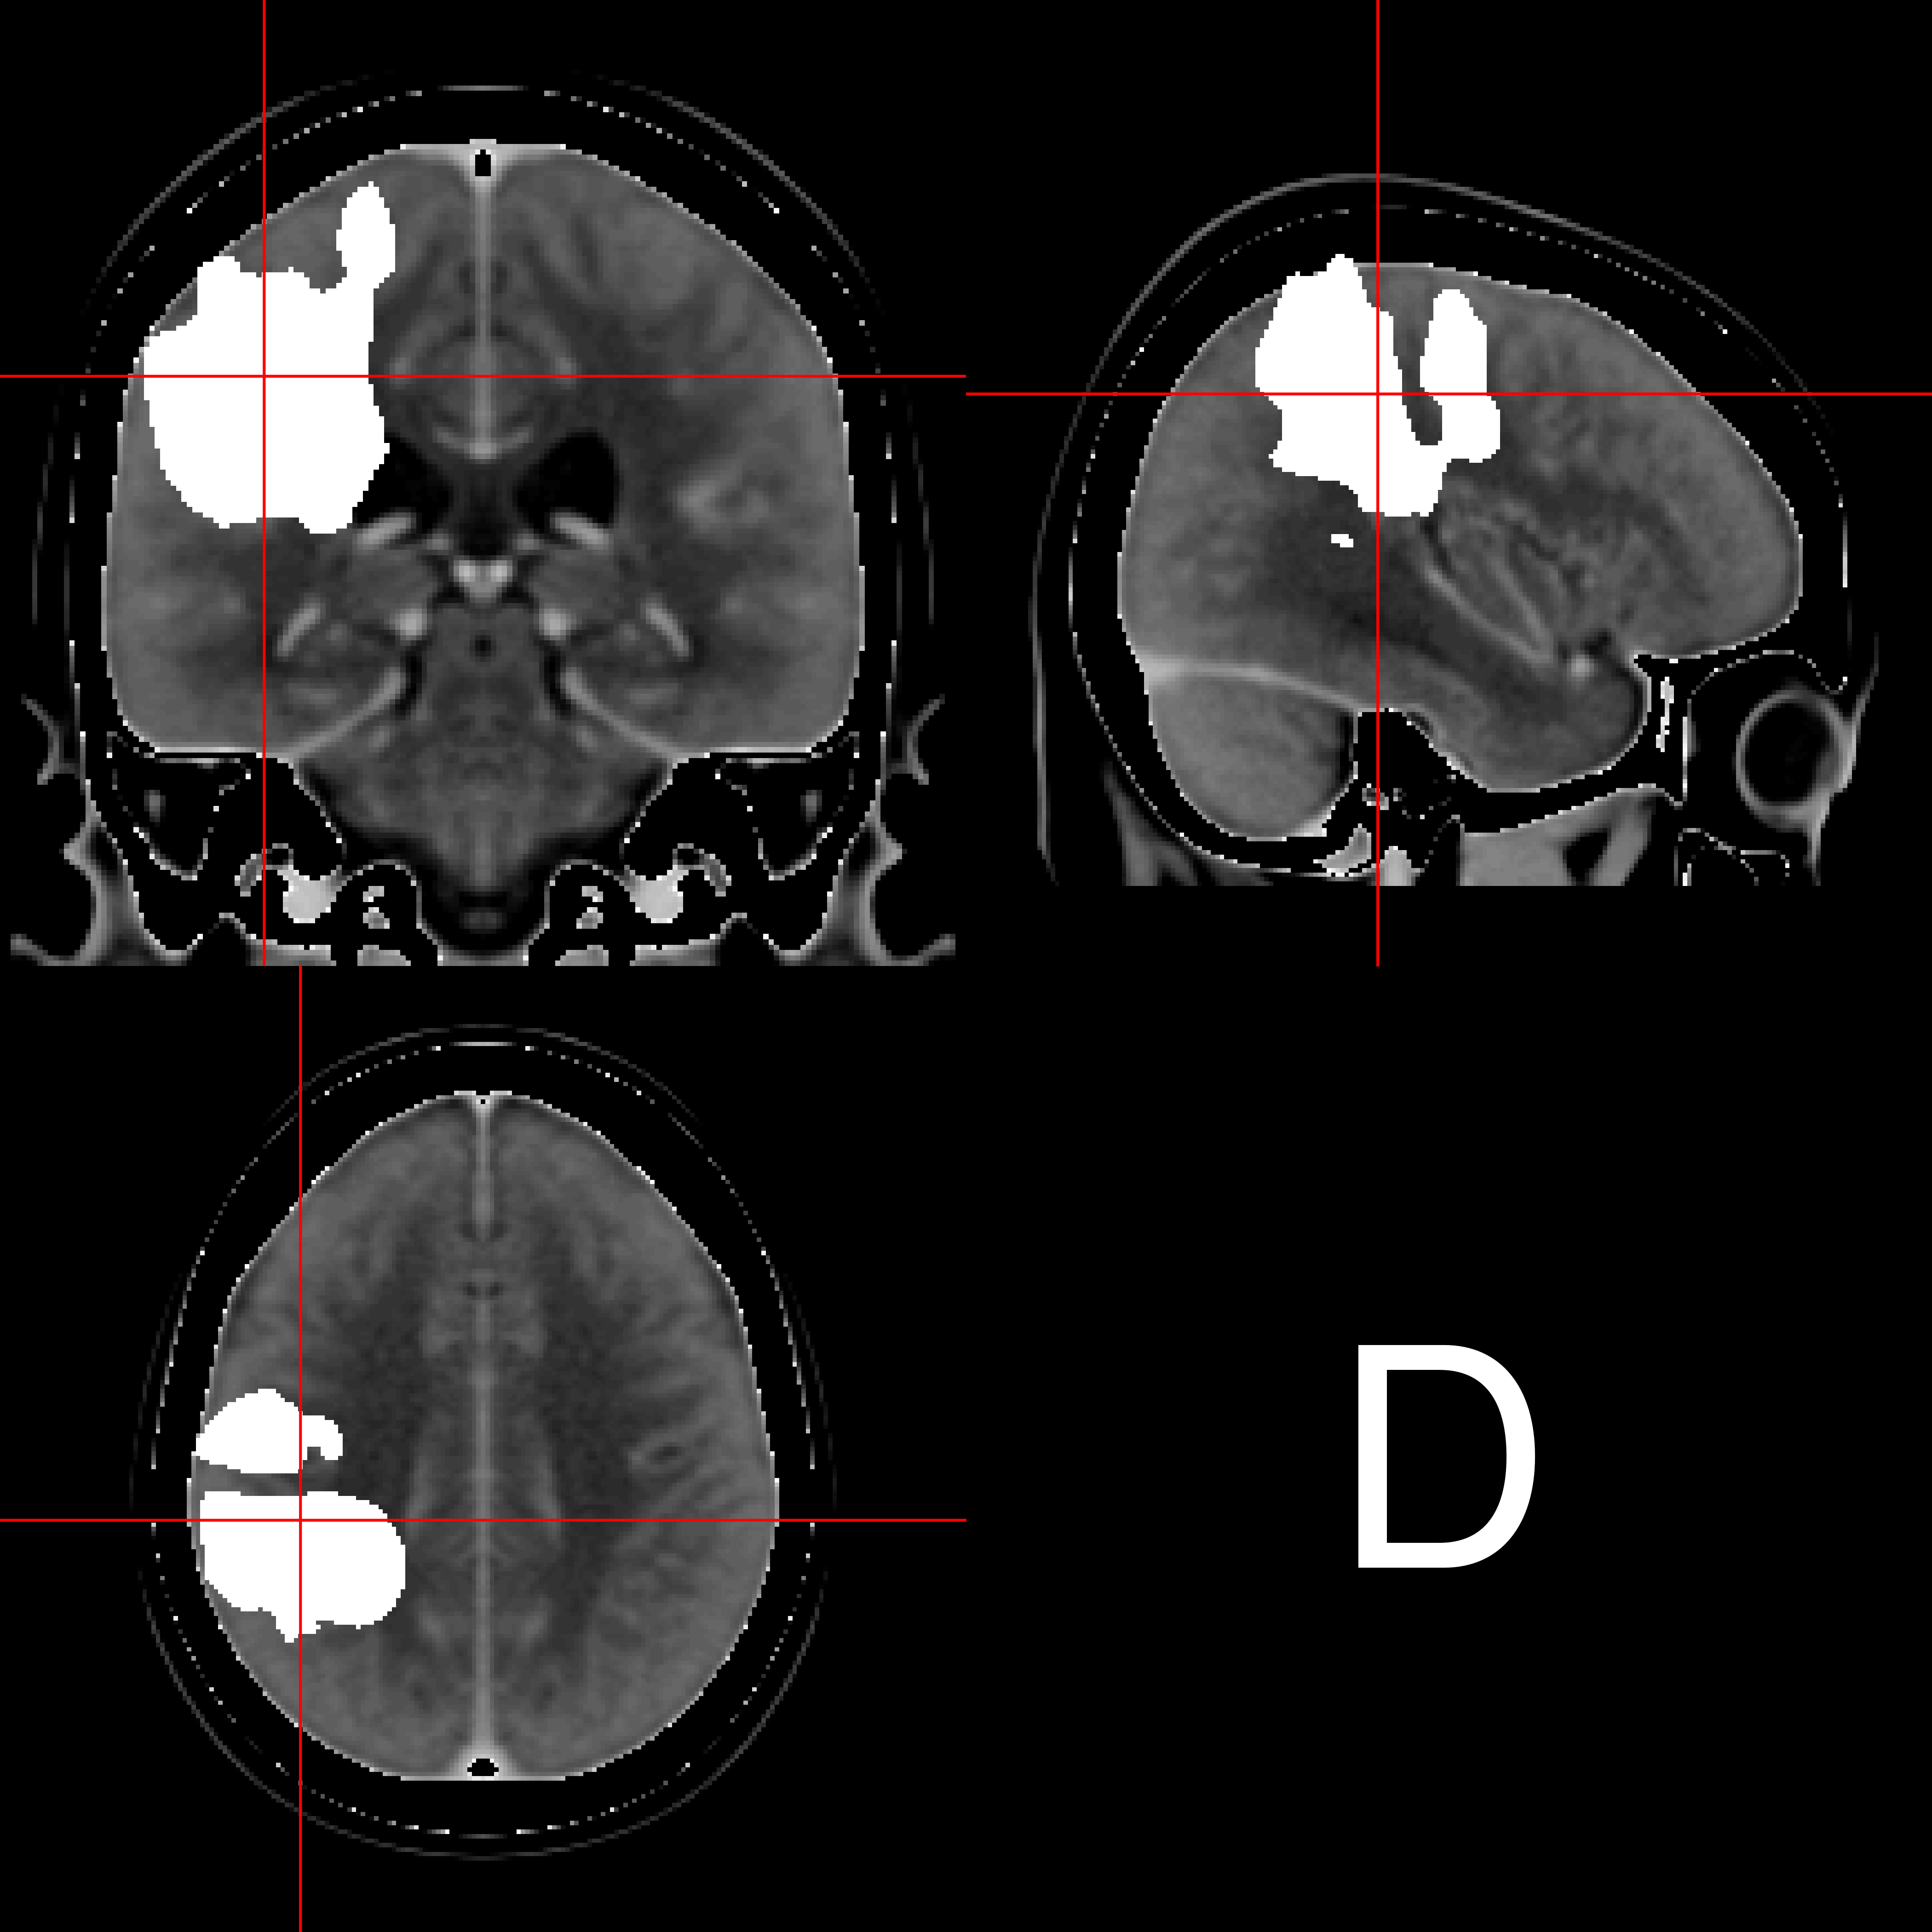
\includegraphics[width=.48\textwidth]{roi_100-362_20100126_1926_CT_2_CT_ROUTINE.png}
 \label{reg:temp1}
} 
  \caption{{\bf Steps of Image Processing}.  The native space image \protect\subref{reg:nat1}, with hemorrhage overlaid in pink, shows variable slice thickness: the top of the brain has smaller voxel sizes (thinner slices) than the bottom of the brain.  The brain-extracted image used for AC-PC alignment is in panel~\protect\subref{reg:ss1}. 
The template-registered image (\protect\subref{reg:co1}) shows the transformation has scaled the brain to the same size as the template.  We see that similar structures, such as the lateral ventricles, are observed on the same axial slice on the patient-level scan compared to the template image, which indicates adequate registration. Panel~\protect\subref{reg:temp1} shows the overlaid hemorrhage mask on the CT template.
  }
  \label{f:reg}
\end{figure}




\begin{figure}[H]
\centering
 \subfloat{
 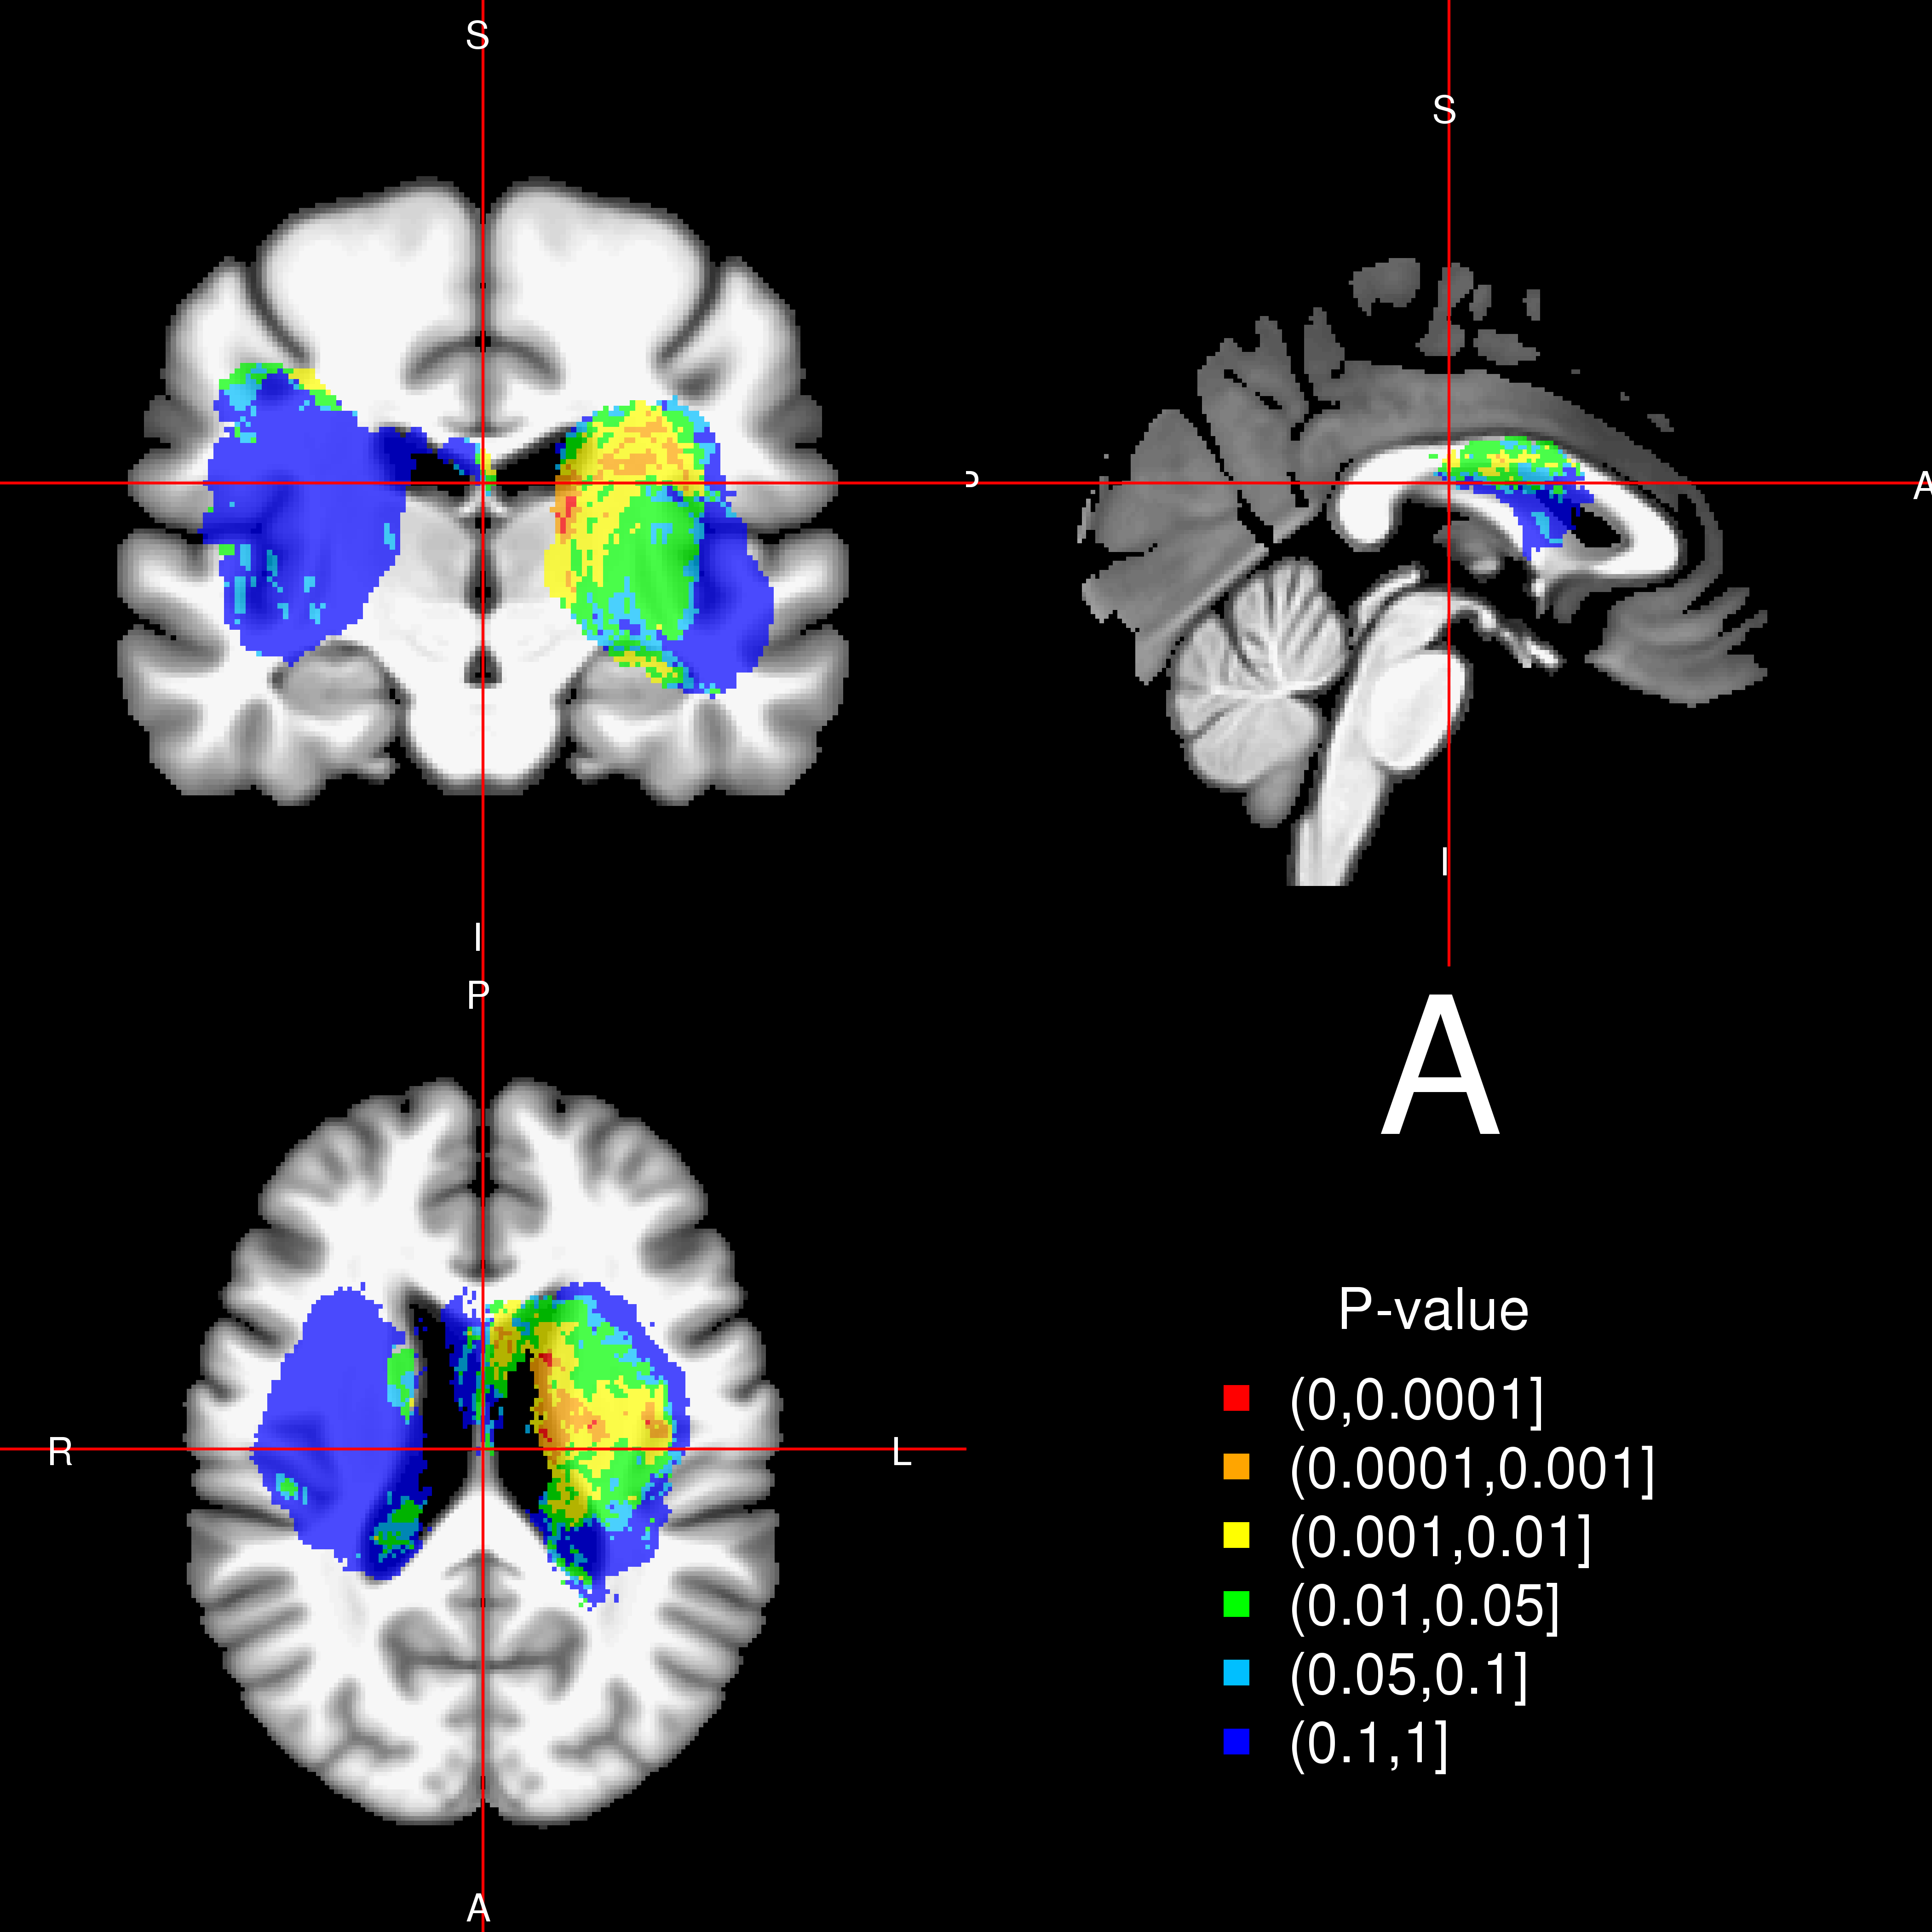
\includegraphics[width=.48\textwidth]{GCS_Regression_Map_heatcol1_t1_Final.png}
 \label{gcsmods:m1}
 }
  \hfill
  \subfloat{
 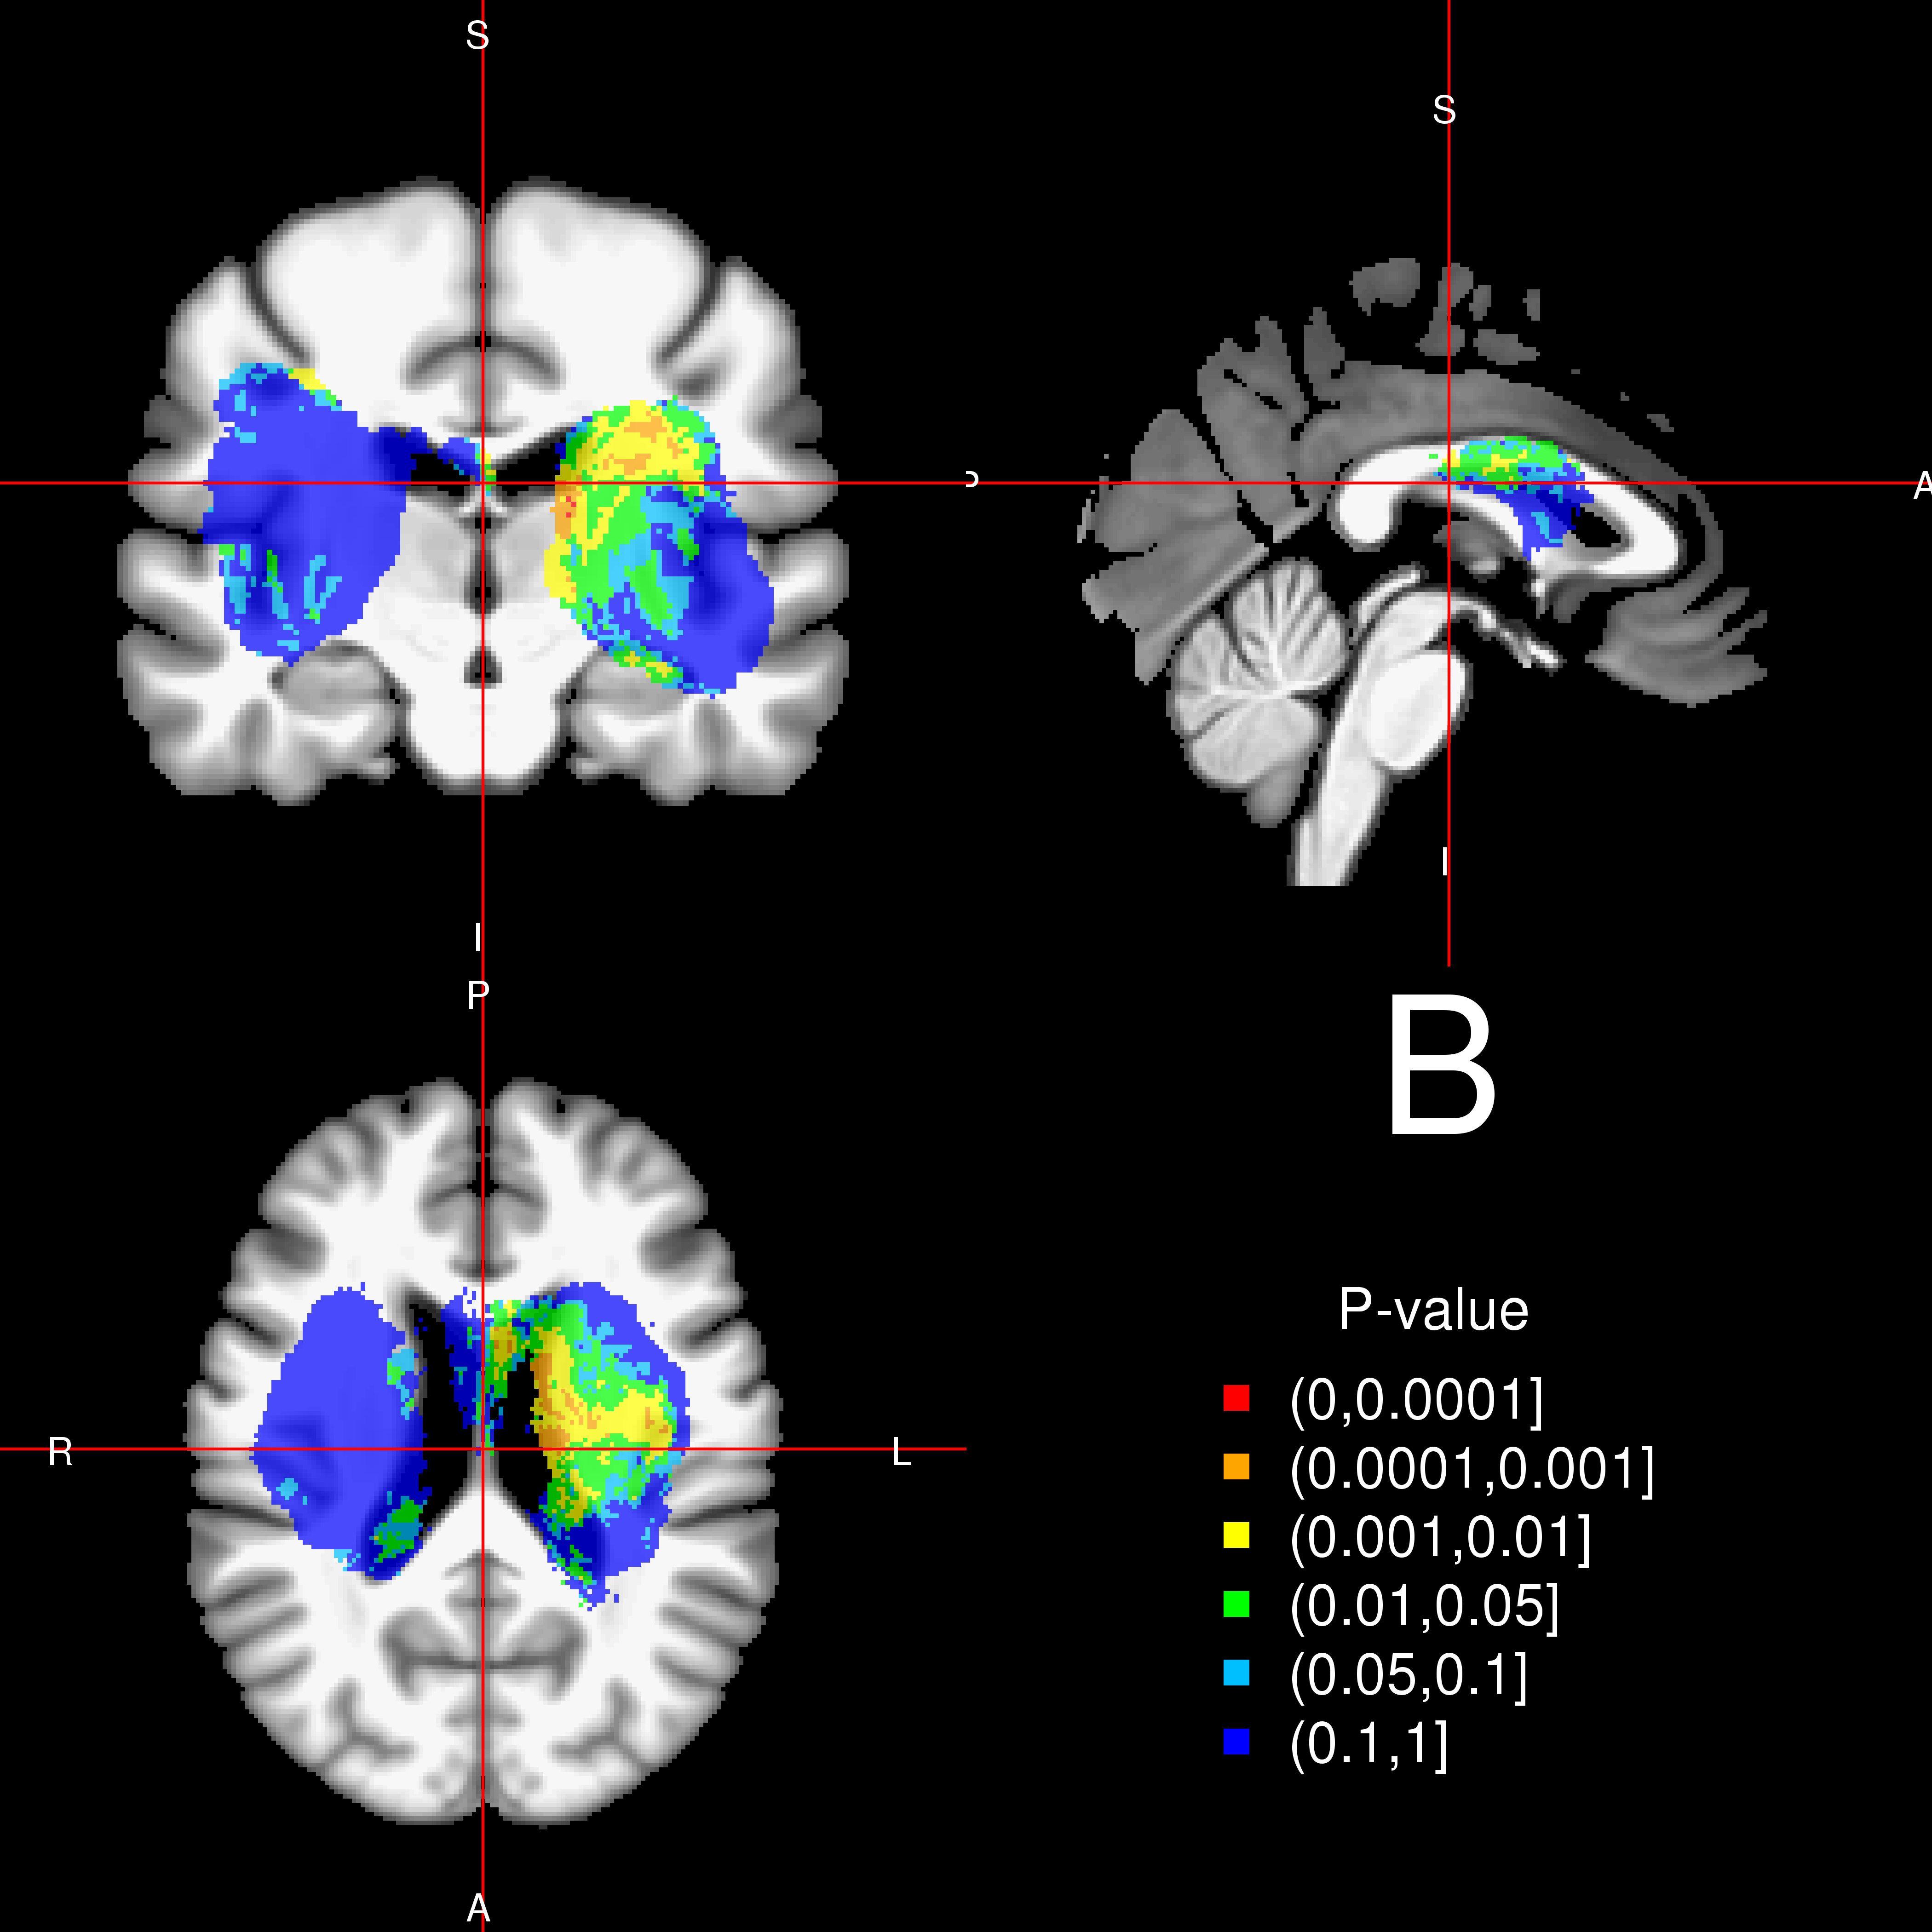
\includegraphics[width=.48\textwidth]{GCS_Regression_Map_heatcol2_t1_Final.png}  
 \label{gcsmods:m2}
 }
  \hfill
  \subfloat{
 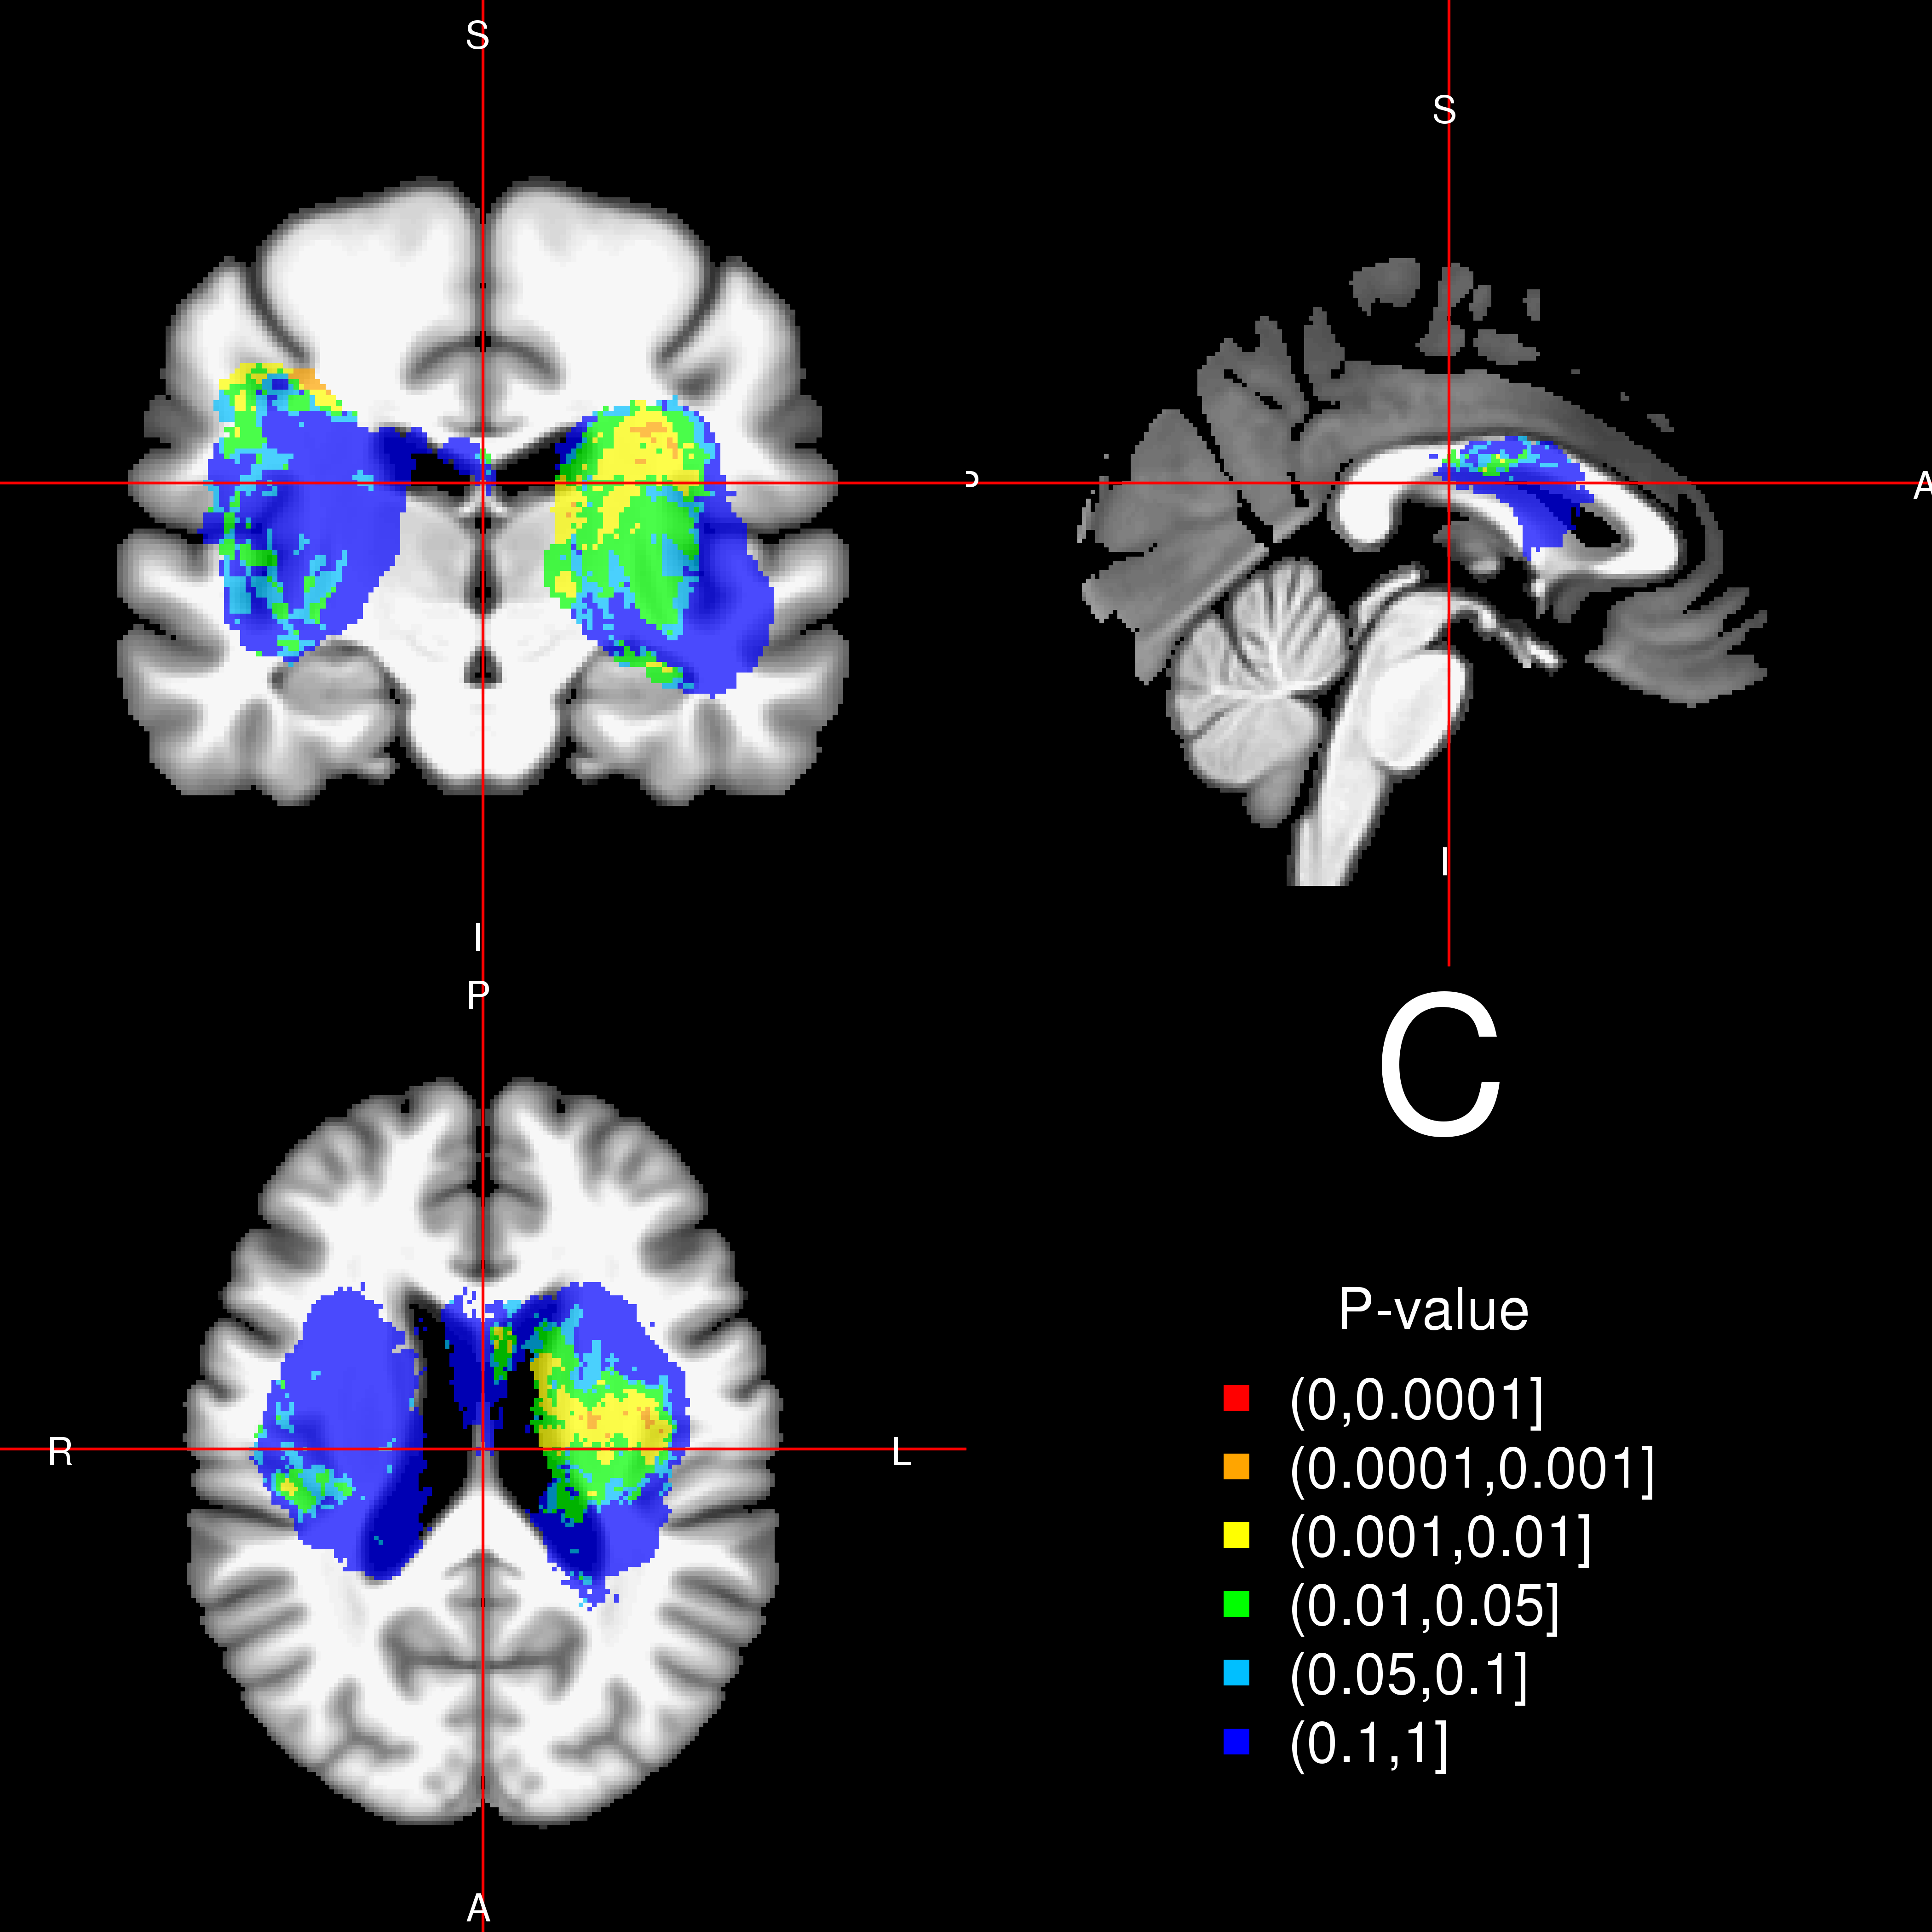
\includegraphics[width=.48\textwidth]{GCS_Regression_Map_heatcol5_t1_Final.png}
 \label{gcsmods:m5}
 }
  \hfill
  \subfloat{
 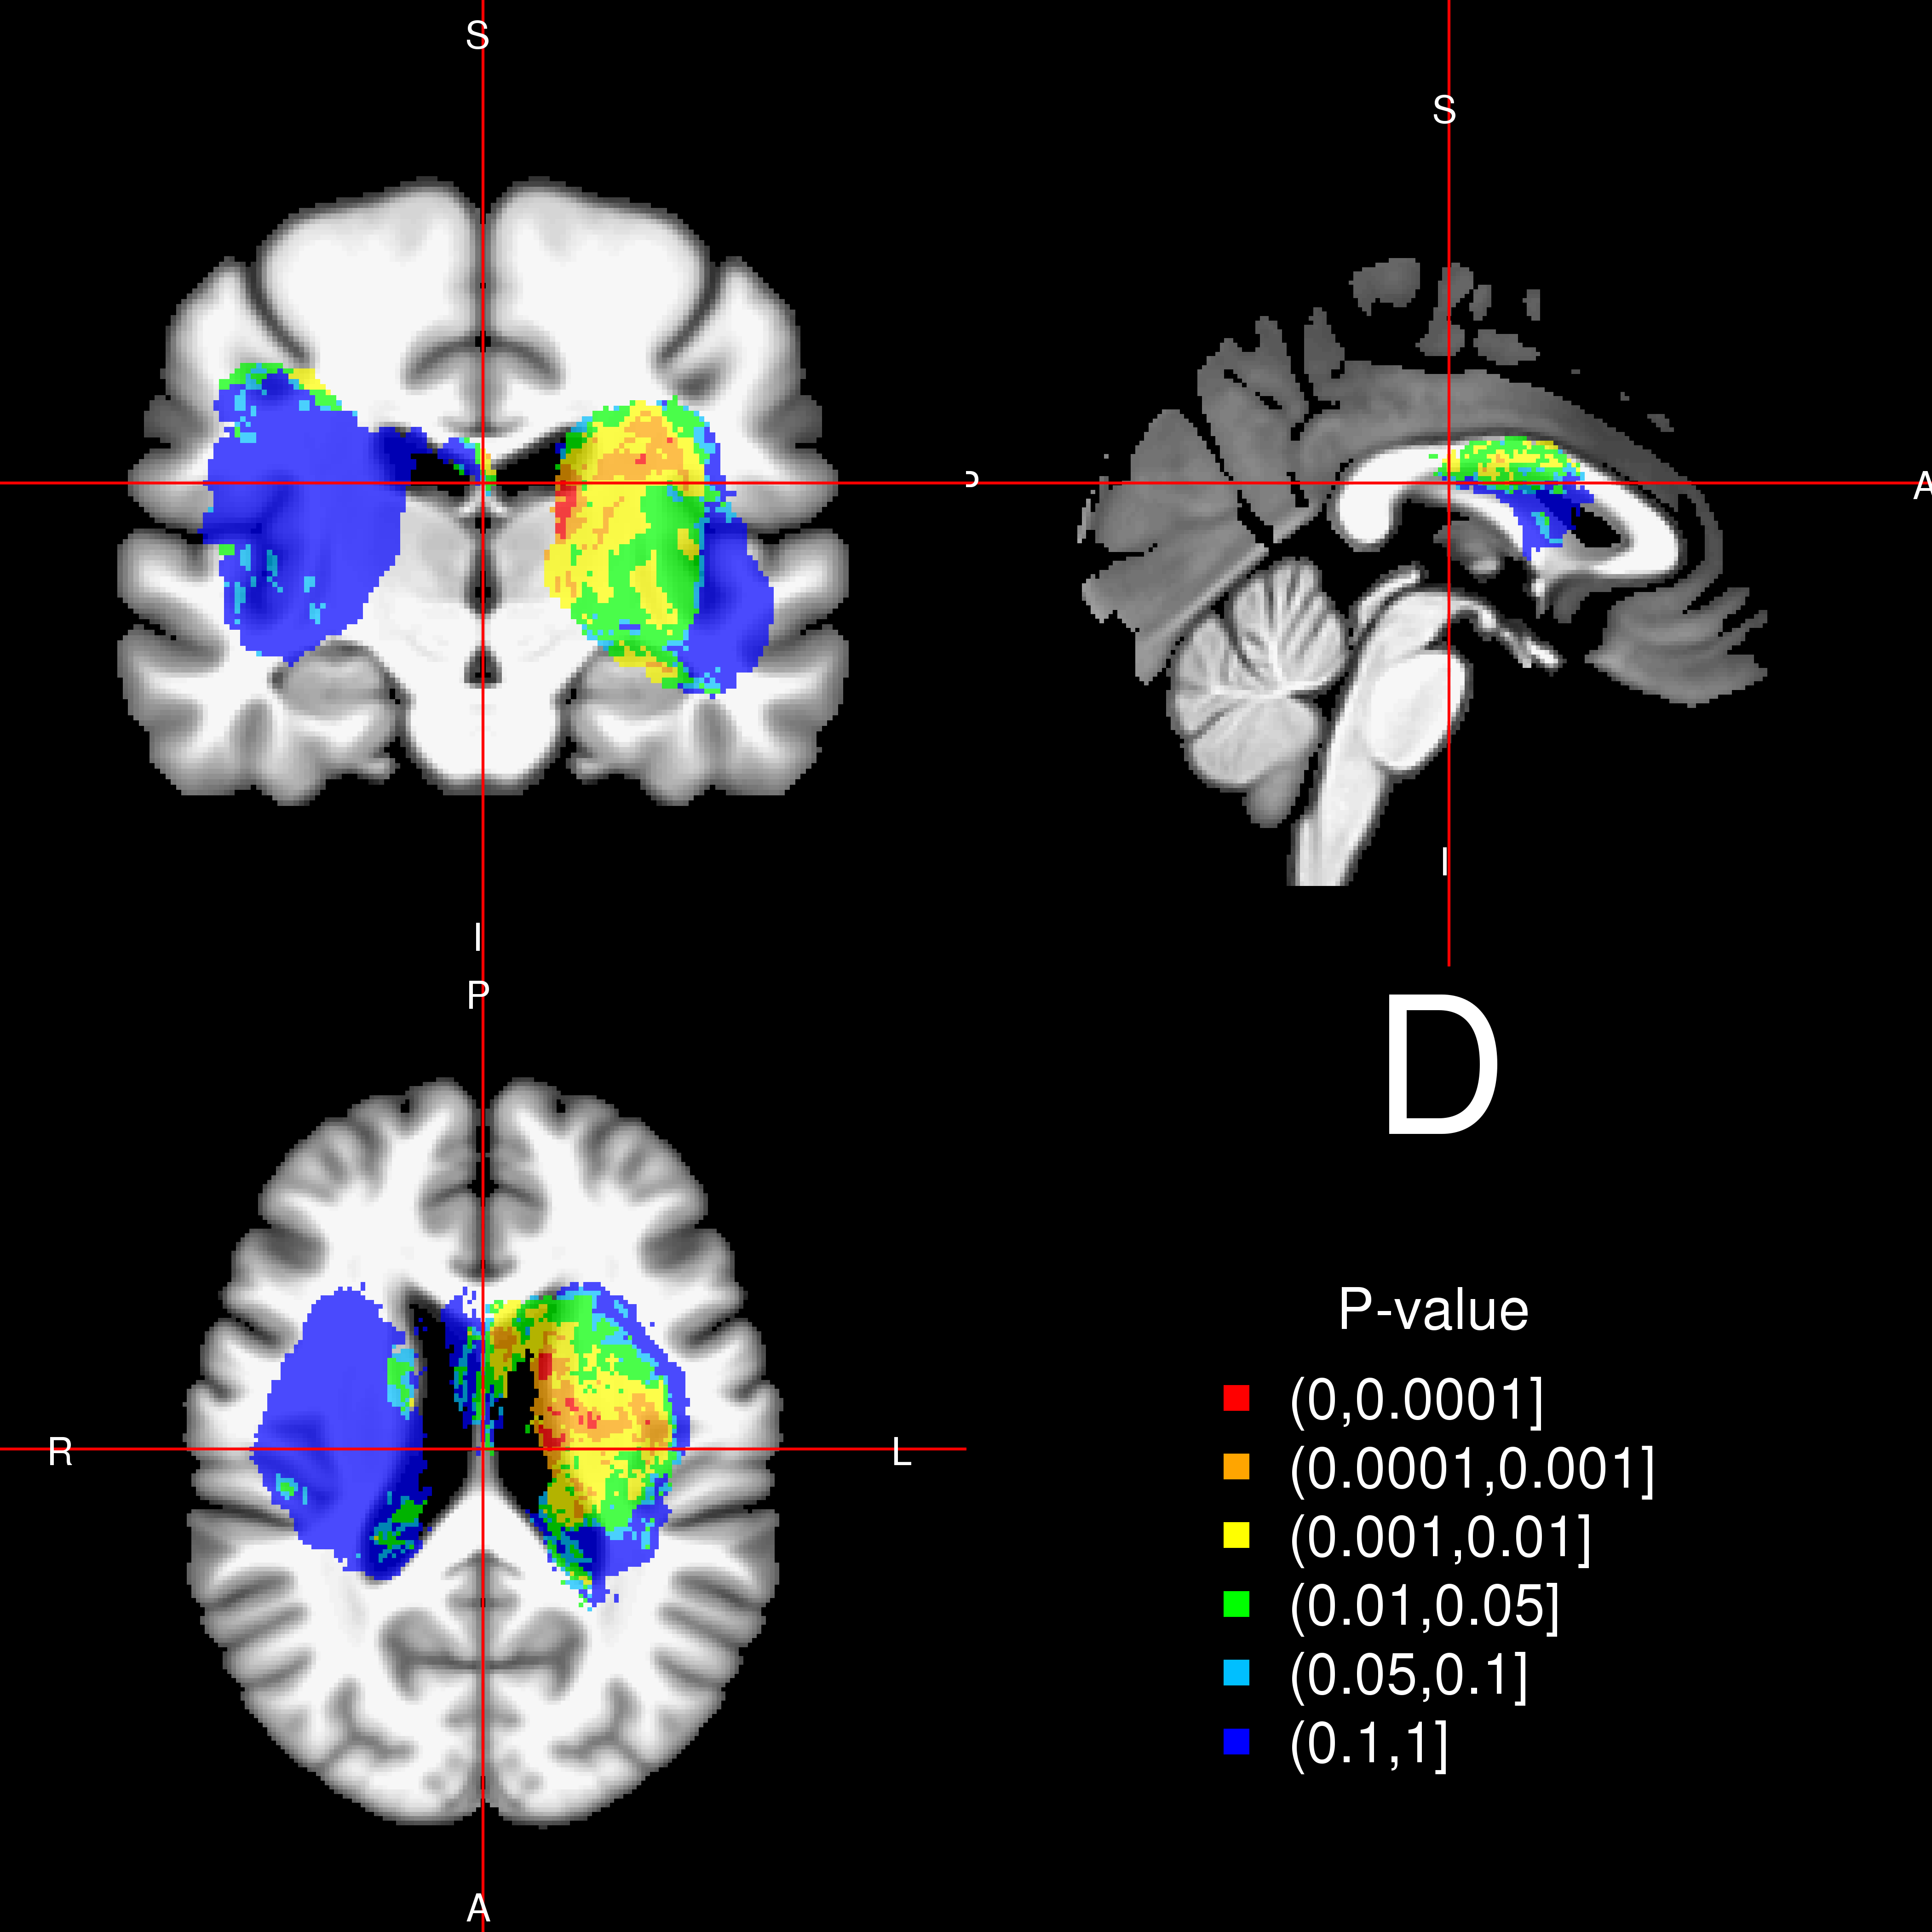
\includegraphics[width=.48\textwidth]{GCS_Regression_Map_heatcol6_t1_Final.png}  
 \label{gcsmods:m6}
 } 
  \caption{{\bf P-value maps for the voxel-wise GCS models.} In the unadjusted linear model (panel~\protect\subref{gcsmods:m1}) and after adjusting for sex (not shown, similar to \protect\subref{gcsmods:m1}) there are voxels with the smallest p-values seem to be near the lateral ventricles.  In models adjusting for age (\protect\subref{gcsmods:m2}), or total baseline ICH volume (not shown, similar to \protect\subref{gcsmods:m6}), or both (\protect\subref{gcsmods:m5}), the p-value relating to GCS scores appear higher (more bluish).  Also, we see the Wilcoxon rank-sum test have smaller p-values for the same area compared to the unadjusted linear model (\protect\subref{gcsmods:m6}).  }
  \label{f:gcsmods}
\end{figure}


\begin{figure}[H]
\centering
  \hfill
  \subfloat{
 \includegraphics[width=.48\textwidth]{{Top_0.01_pvalues_Final_symm}.png}  
 \label{pvals:nihss_symm}
 }
  \hfill
  \subfloat{
 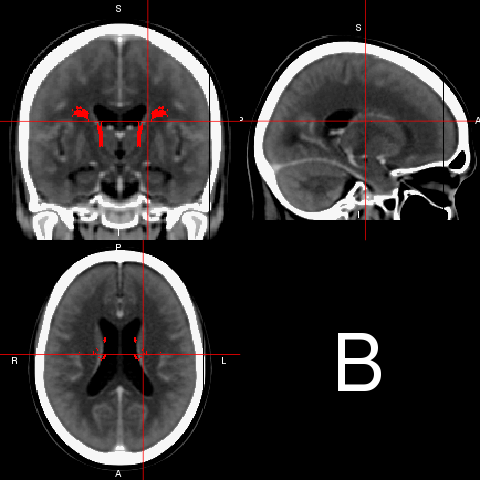
\includegraphics[width=.48\textwidth]{GCS_Top_1000_pvalues_Final_symm.png}  
 \label{pvals:gcs_symm}
 } 
 \newline
  \hfill
  \subfloat{
 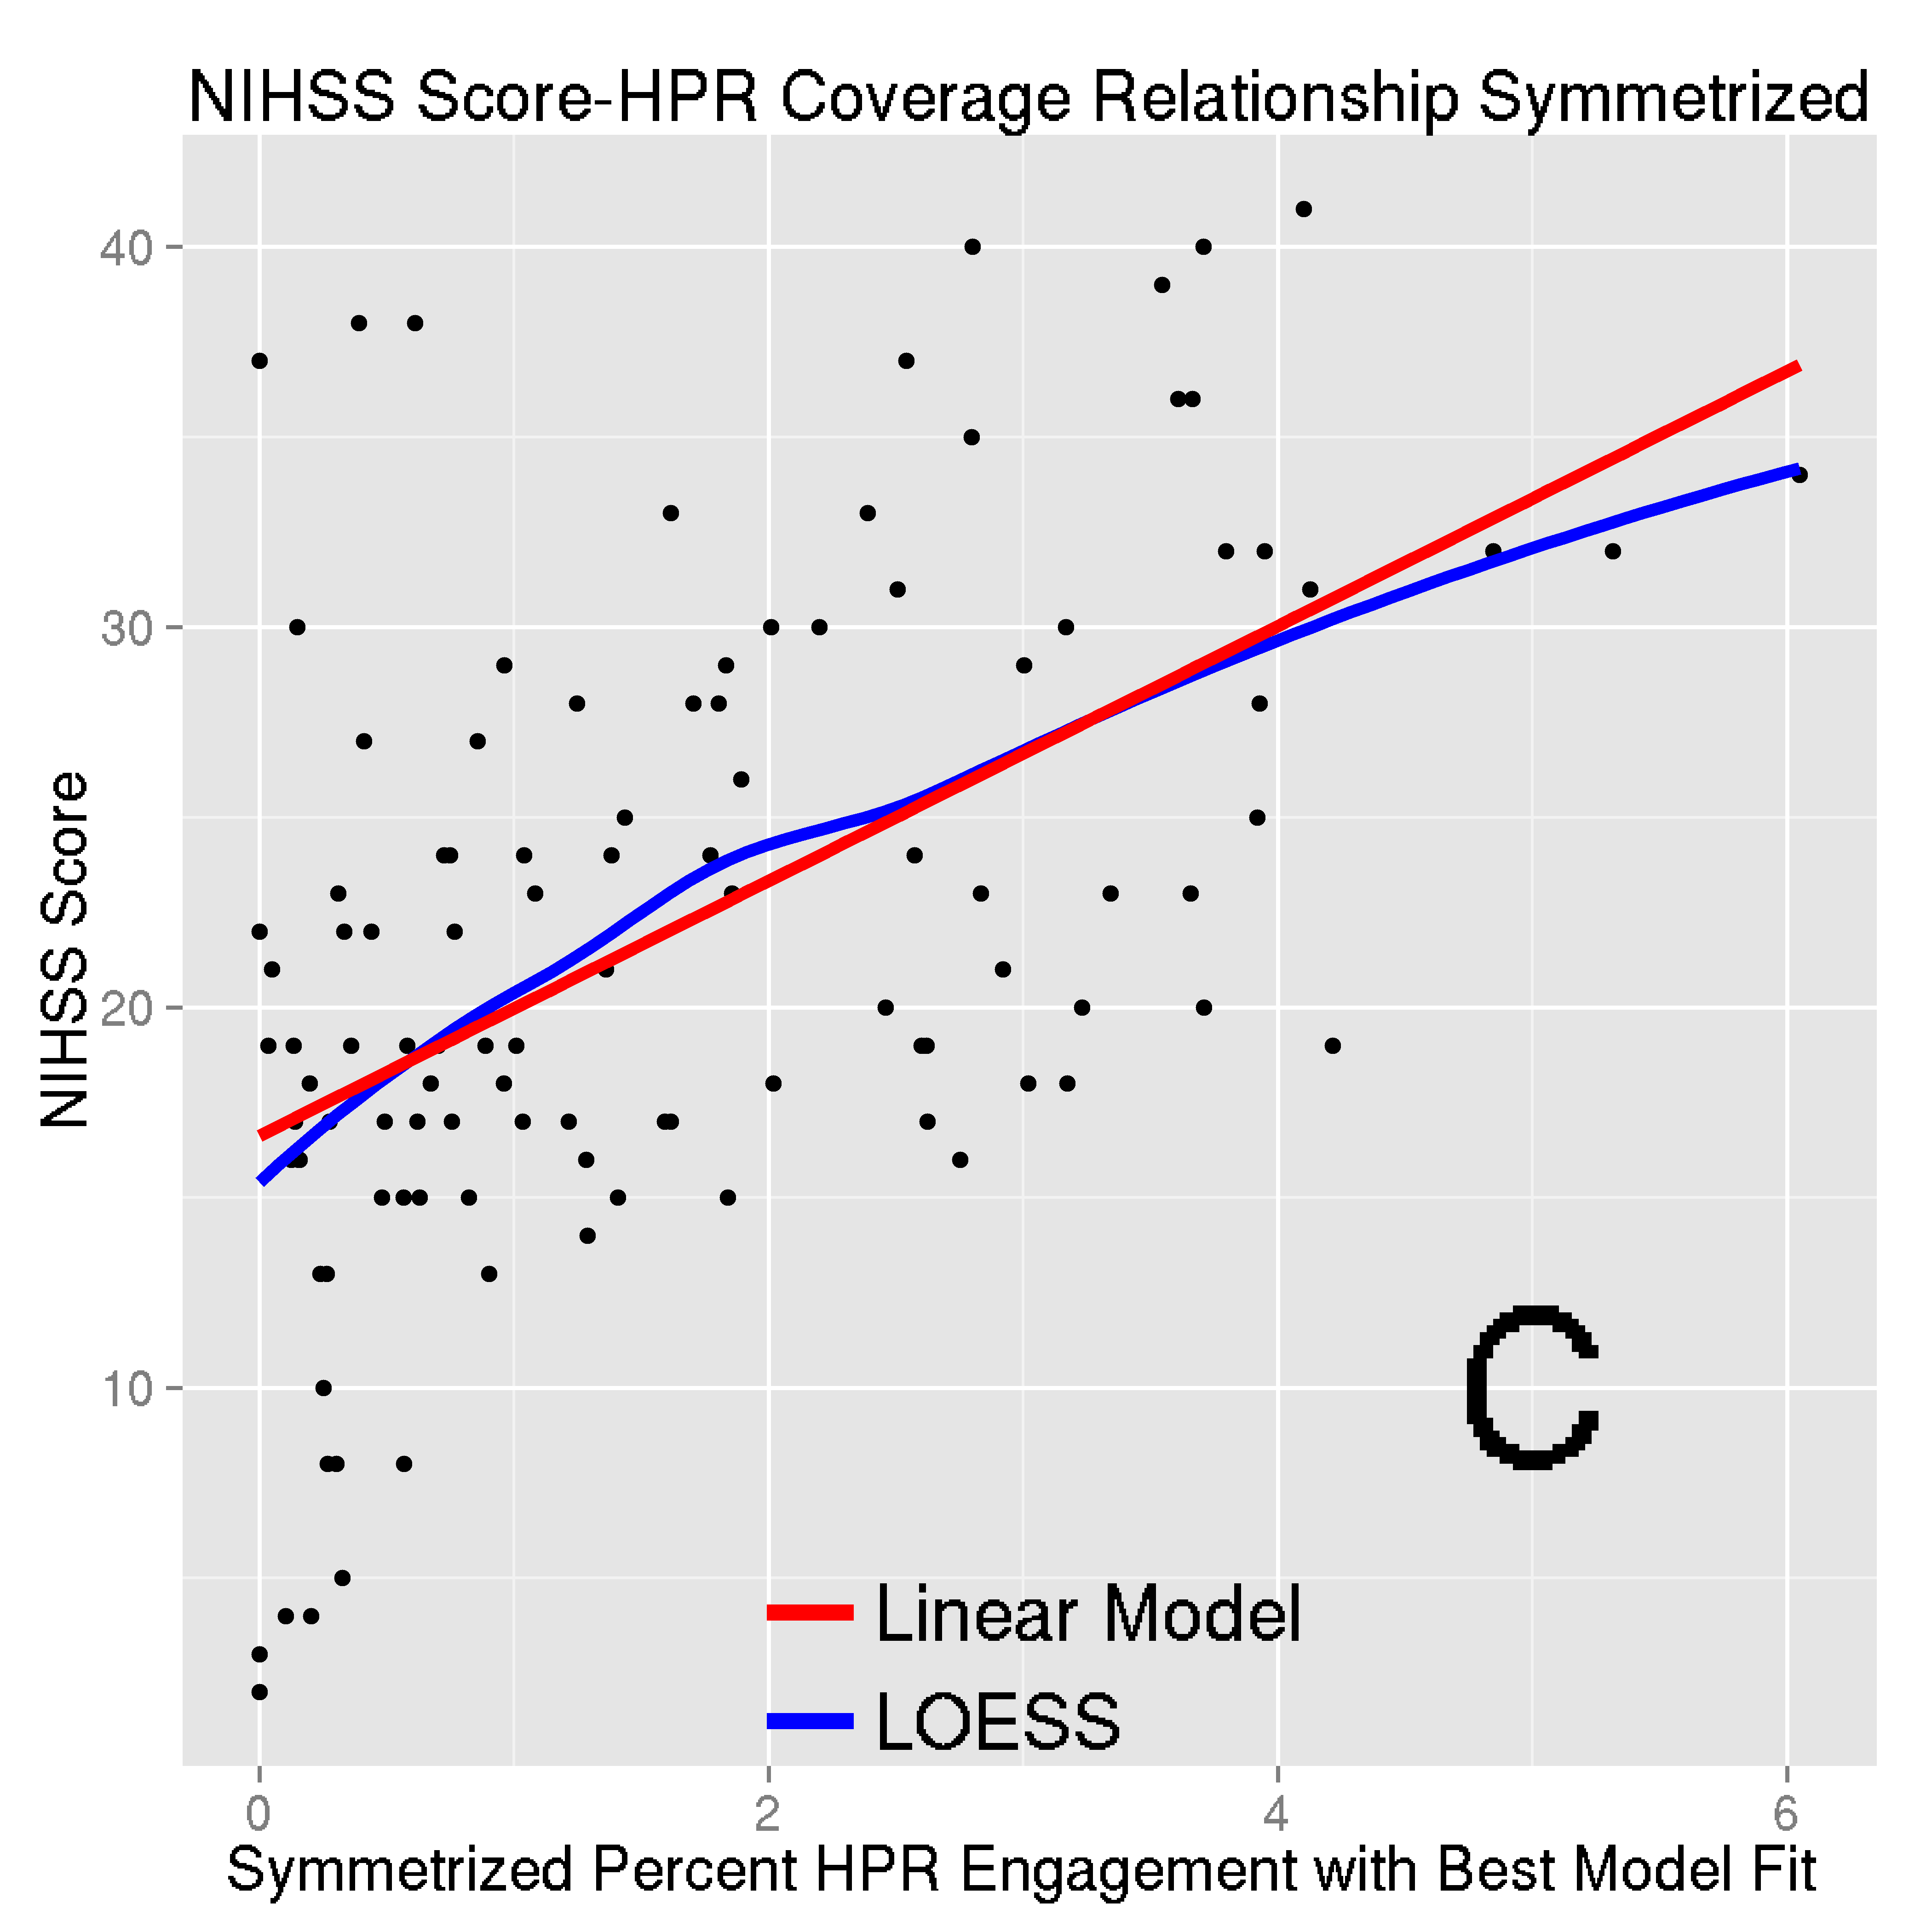
\includegraphics[width=.48\textwidth]{Regress_ROI_NIHSS_Best_Model_Symmetrized.png}  
 \label{pvals:regnihss_symm}
 }
  \hfill
  \subfloat{
 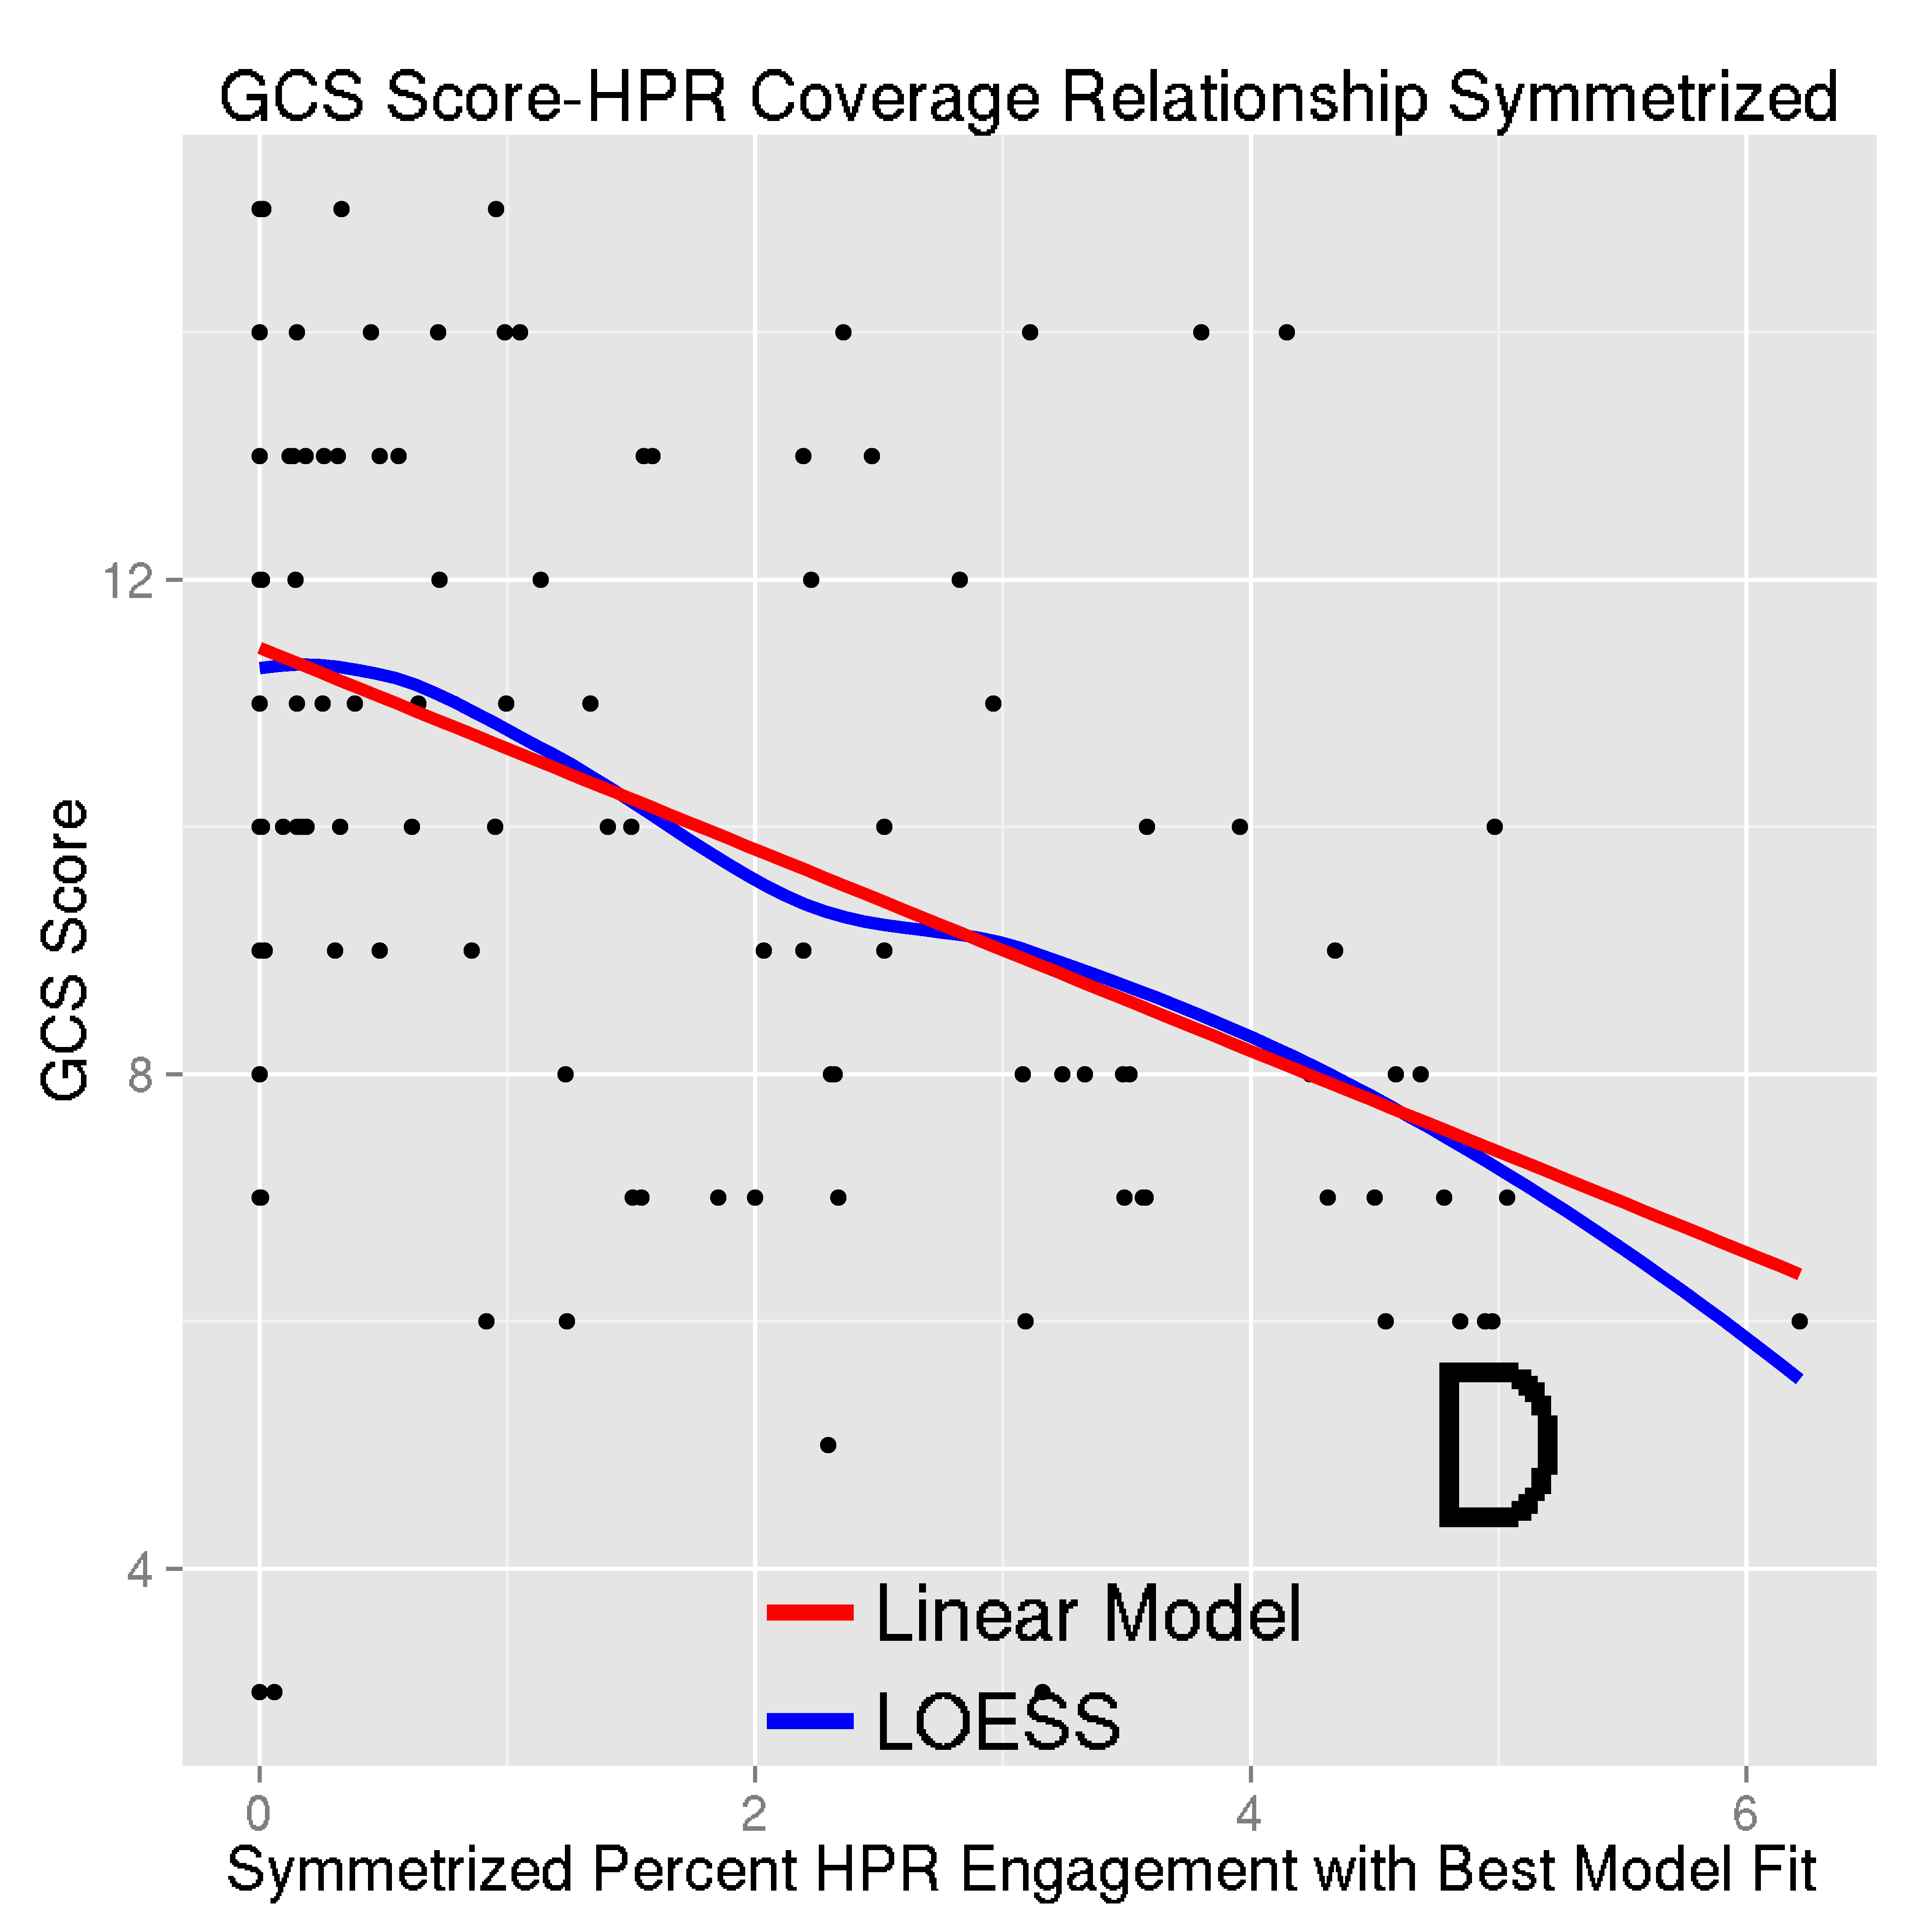
\includegraphics[width=.48\textwidth]{Regress_ROI_GCS_Best_Model_Symmetrized.png}  
 \label{pvals:reggcs_symm}
 } 
 \newline 
  \caption{{\bf Highest Predictive Region (HPR) Analysis with Symmetrized HPR.}  HPR were symmetrized by including voxels in the HPR and the voxel on the contra-lateral side.  Panels~\protect\subref{pvals:nihss_symm} and~\protect\subref{pvals:gcs_symm} correspond to the symmetrized HPR  for NIHSS (Figure~\ref{f:roi}\protect\subref{pvals:nihss}) and GCS (Figure~\ref{f:roi}\protect\subref{pvals:gcs}), respectively.  Panels~\protect\subref{pvals:regnihss} and~\protect\subref{pvals:reggcs} plot the symmetrized HPR coverage--severity score relationship.  The larger the coverage the higher (more severe stroke) NIHSS score and the lower (deeper unconsciousness) the GCS score.  
}
  \label{f:roi_symm}
\end{figure}






\end{document}

ADD:
Matching of patients
Results from threshold
More introduction

